\documentclass[twoside]{book}

% Packages required by doxygen
\usepackage{fixltx2e}
\usepackage{calc}
\usepackage{doxygen}
\usepackage[export]{adjustbox} % also loads graphicx
\usepackage{graphicx}
\usepackage[utf8]{inputenc}
\usepackage{makeidx}
\usepackage{multicol}
\usepackage{multirow}
\PassOptionsToPackage{warn}{textcomp}
\usepackage{textcomp}
\usepackage[nointegrals]{wasysym}
\usepackage[table]{xcolor}

% Font selection
\usepackage[T1]{fontenc}
\usepackage[scaled=.90]{helvet}
\usepackage{courier}
\usepackage{amssymb}
\usepackage{sectsty}
\renewcommand{\familydefault}{\sfdefault}
\allsectionsfont{%
  \fontseries{bc}\selectfont%
  \color{darkgray}%
}
\renewcommand{\DoxyLabelFont}{%
  \fontseries{bc}\selectfont%
  \color{darkgray}%
}
\newcommand{\+}{\discretionary{\mbox{\scriptsize$\hookleftarrow$}}{}{}}

% Page & text layout
\usepackage{geometry}
\geometry{%
  a4paper,%
  top=2.5cm,%
  bottom=2.5cm,%
  left=2.5cm,%
  right=2.5cm%
}
\tolerance=750
\hfuzz=15pt
\hbadness=750
\setlength{\emergencystretch}{15pt}
\setlength{\parindent}{0cm}
\setlength{\parskip}{0.2cm}
\makeatletter
\renewcommand{\paragraph}{%
  \@startsection{paragraph}{4}{0ex}{-1.0ex}{1.0ex}{%
    \normalfont\normalsize\bfseries\SS@parafont%
  }%
}
\renewcommand{\subparagraph}{%
  \@startsection{subparagraph}{5}{0ex}{-1.0ex}{1.0ex}{%
    \normalfont\normalsize\bfseries\SS@subparafont%
  }%
}
\makeatother

% Headers & footers
\usepackage{fancyhdr}
\pagestyle{fancyplain}
\fancyhead[LE]{\fancyplain{}{\bfseries\thepage}}
\fancyhead[CE]{\fancyplain{}{}}
\fancyhead[RE]{\fancyplain{}{\bfseries\leftmark}}
\fancyhead[LO]{\fancyplain{}{\bfseries\rightmark}}
\fancyhead[CO]{\fancyplain{}{}}
\fancyhead[RO]{\fancyplain{}{\bfseries\thepage}}
\fancyfoot[LE]{\fancyplain{}{}}
\fancyfoot[CE]{\fancyplain{}{}}
\fancyfoot[RE]{\fancyplain{}{\bfseries\scriptsize Generated on Sun Feb 12 2017 18\+:49\+:03 for My Project by Doxygen }}
\fancyfoot[LO]{\fancyplain{}{\bfseries\scriptsize Generated on Sun Feb 12 2017 18\+:49\+:03 for My Project by Doxygen }}
\fancyfoot[CO]{\fancyplain{}{}}
\fancyfoot[RO]{\fancyplain{}{}}
\renewcommand{\footrulewidth}{0.4pt}
\renewcommand{\chaptermark}[1]{%
  \markboth{#1}{}%
}
\renewcommand{\sectionmark}[1]{%
  \markright{\thesection\ #1}%
}

% Indices & bibliography
\usepackage{natbib}
\usepackage[titles]{tocloft}
\setcounter{tocdepth}{3}
\setcounter{secnumdepth}{5}
\makeindex

% Hyperlinks (required, but should be loaded last)
\usepackage{ifpdf}
\ifpdf
  \usepackage[pdftex,pagebackref=true]{hyperref}
\else
  \usepackage[ps2pdf,pagebackref=true]{hyperref}
\fi
\hypersetup{%
  colorlinks=true,%
  linkcolor=blue,%
  citecolor=blue,%
  unicode%
}

% Custom commands
\newcommand{\clearemptydoublepage}{%
  \newpage{\pagestyle{empty}\cleardoublepage}%
}


%===== C O N T E N T S =====

\begin{document}

% Titlepage & ToC
\hypersetup{pageanchor=false,
             bookmarks=true,
             bookmarksnumbered=true,
             pdfencoding=unicode
            }
\pagenumbering{roman}
\begin{titlepage}
\vspace*{7cm}
\begin{center}%
{\Large My Project }\\
\vspace*{1cm}
{\large Generated by Doxygen 1.8.9.1}\\
\vspace*{0.5cm}
{\small Sun Feb 12 2017 18:49:03}\\
\end{center}
\end{titlepage}
\clearemptydoublepage
\tableofcontents
\clearemptydoublepage
\pagenumbering{arabic}
\hypersetup{pageanchor=true}

%--- Begin generated contents ---
\chapter{Hierarchical Index}
\section{Class Hierarchy}
This inheritance list is sorted roughly, but not completely, alphabetically\+:\begin{DoxyCompactList}
\item \contentsline{section}{Interfaces.\+Container}{\pageref{interfaceInterfaces_1_1Container}}{}
\begin{DoxyCompactList}
\item \contentsline{section}{Cars.\+Container\+Part}{\pageref{classCars_1_1ContainerPart}}{}
\begin{DoxyCompactList}
\item \contentsline{section}{Brake\+Parts.\+Master\+Cylinder}{\pageref{classBrakeParts_1_1MasterCylinder}}{}
\item \contentsline{section}{Drive\+Train\+Parts.\+Transmission}{\pageref{classDriveTrainParts_1_1Transmission}}{}
\item \contentsline{section}{Electrical\+Parts.\+Battery}{\pageref{classElectricalParts_1_1Battery}}{}
\item \contentsline{section}{Fuel\+System\+Parts.\+Tank}{\pageref{classFuelSystemParts_1_1Tank}}{}
\item \contentsline{section}{Suspension\+Parts.\+Tire}{\pageref{classSuspensionParts_1_1Tire}}{}
\end{DoxyCompactList}
\item \contentsline{section}{Power\+Train\+Parts.\+Motor}{\pageref{classPowerTrainParts_1_1Motor}}{}
\end{DoxyCompactList}
\item \contentsline{section}{Interfaces.\+Electronic}{\pageref{interfaceInterfaces_1_1Electronic}}{}
\begin{DoxyCompactList}
\item \contentsline{section}{Cars.\+Electronic\+Part}{\pageref{classCars_1_1ElectronicPart}}{}
\begin{DoxyCompactList}
\item \contentsline{section}{Fuel\+System\+Parts.\+Pump}{\pageref{classFuelSystemParts_1_1Pump}}{}
\item \contentsline{section}{Ignition\+Parts.\+Computer}{\pageref{classIgnitionParts_1_1Computer}}{}
\item \contentsline{section}{Ignition\+Parts.\+Ignition\+Switch}{\pageref{classIgnitionParts_1_1IgnitionSwitch}}{}
\item \contentsline{section}{Ignition\+Parts.\+Starter}{\pageref{classIgnitionParts_1_1Starter}}{}
\item \contentsline{section}{Power\+Train\+Parts.\+Motor}{\pageref{classPowerTrainParts_1_1Motor}}{}
\end{DoxyCompactList}
\item \contentsline{section}{Cars.\+Electronic\+System}{\pageref{classCars_1_1ElectronicSystem}}{}
\begin{DoxyCompactList}
\item \contentsline{section}{Cars.\+Car}{\pageref{classCars_1_1Car}}{}
\item \contentsline{section}{Systems.\+Electrical}{\pageref{classSystems_1_1Electrical}}{}
\item \contentsline{section}{Systems.\+Ignition}{\pageref{classSystems_1_1Ignition}}{}
\end{DoxyCompactList}
\end{DoxyCompactList}
\item \contentsline{section}{Interfaces.\+Iterative}{\pageref{interfaceInterfaces_1_1Iterative}}{}
\begin{DoxyCompactList}
\item \contentsline{section}{Ignition\+Parts.\+Ignition\+Switch}{\pageref{classIgnitionParts_1_1IgnitionSwitch}}{}
\item \contentsline{section}{Systems.\+Fuel}{\pageref{classSystems_1_1Fuel}}{}
\item \contentsline{section}{Systems.\+Ignition}{\pageref{classSystems_1_1Ignition}}{}
\end{DoxyCompactList}
\item \contentsline{section}{Enums.\+Location}{\pageref{enumEnums_1_1Location}}{}
\item \contentsline{section}{Enums.\+Part\+Catagory}{\pageref{enumEnums_1_1PartCatagory}}{}
\item Runnable\begin{DoxyCompactList}
\item \contentsline{section}{Cars.\+Worker\+Thread}{\pageref{classCars_1_1WorkerThread}}{}
\end{DoxyCompactList}
\item \contentsline{section}{Cars.\+Simulator}{\pageref{classCars_1_1Simulator}}{}
\item \contentsline{section}{Enums.\+Status}{\pageref{enumEnums_1_1Status}}{}
\item \contentsline{section}{Interfaces.\+System}{\pageref{interfaceInterfaces_1_1System}}{}
\begin{DoxyCompactList}
\item \contentsline{section}{Cars.\+Car\+Part}{\pageref{classCars_1_1CarPart}}{}
\begin{DoxyCompactList}
\item \contentsline{section}{Brake\+Parts.\+Caliper}{\pageref{classBrakeParts_1_1Caliper}}{}
\item \contentsline{section}{Brake\+Parts.\+Pads}{\pageref{classBrakeParts_1_1Pads}}{}
\item \contentsline{section}{Brake\+Parts.\+Rotor}{\pageref{classBrakeParts_1_1Rotor}}{}
\item \contentsline{section}{Cars.\+Container\+Part}{\pageref{classCars_1_1ContainerPart}}{}
\item \contentsline{section}{Cars.\+Electronic\+Part}{\pageref{classCars_1_1ElectronicPart}}{}
\item \contentsline{section}{Connectors.\+Line}{\pageref{classConnectors_1_1Line}}{}
\item \contentsline{section}{Connectors.\+Wire}{\pageref{classConnectors_1_1Wire}}{}
\item \contentsline{section}{Drive\+Train\+Parts.\+Drive\+Axel}{\pageref{classDriveTrainParts_1_1DriveAxel}}{}
\item \contentsline{section}{Drive\+Train\+Parts.\+Drive\+Shaft}{\pageref{classDriveTrainParts_1_1DriveShaft}}{}
\item \contentsline{section}{Electrical\+Parts.\+Alternator}{\pageref{classElectricalParts_1_1Alternator}}{}
\item \contentsline{section}{Fuel\+System\+Parts.\+Filter}{\pageref{classFuelSystemParts_1_1Filter}}{}
\item \contentsline{section}{Power\+Train\+Parts.\+Air\+Filter}{\pageref{classPowerTrainParts_1_1AirFilter}}{}
\item \contentsline{section}{Power\+Train\+Parts.\+Oil\+Filter}{\pageref{classPowerTrainParts_1_1OilFilter}}{}
\item \contentsline{section}{Suspension\+Parts.\+Rim}{\pageref{classSuspensionParts_1_1Rim}}{}
\item \contentsline{section}{Suspension\+Parts.\+Shock}{\pageref{classSuspensionParts_1_1Shock}}{}
\item \contentsline{section}{Suspension\+Parts.\+Strut}{\pageref{classSuspensionParts_1_1Strut}}{}
\end{DoxyCompactList}
\item \contentsline{section}{Cars.\+Electronic\+System}{\pageref{classCars_1_1ElectronicSystem}}{}
\item \contentsline{section}{Fuel\+System\+Parts.\+Tank}{\pageref{classFuelSystemParts_1_1Tank}}{}
\item \contentsline{section}{Systems.\+Brakes}{\pageref{classSystems_1_1Brakes}}{}
\item \contentsline{section}{Systems.\+Drive\+Train}{\pageref{classSystems_1_1DriveTrain}}{}
\item \contentsline{section}{Systems.\+Electrical}{\pageref{classSystems_1_1Electrical}}{}
\item \contentsline{section}{Systems.\+Fuel}{\pageref{classSystems_1_1Fuel}}{}
\item \contentsline{section}{Systems.\+Power\+Train}{\pageref{classSystems_1_1PowerTrain}}{}
\item \contentsline{section}{Systems.\+Suspension}{\pageref{classSystems_1_1Suspension}}{}
\end{DoxyCompactList}
\item Vector\begin{DoxyCompactList}
\item \contentsline{section}{Cars.\+Car\+Part\+Vector}{\pageref{classCars_1_1CarPartVector}}{}
\end{DoxyCompactList}
\end{DoxyCompactList}

\chapter{Class Index}
\section{Class List}
Here are the classes, structs, unions and interfaces with brief descriptions\+:\begin{DoxyCompactList}
\item\contentsline{section}{\hyperlink{classPowerTrainParts_1_1AirFilter}{Power\+Train\+Parts.\+Air\+Filter} }{\pageref{classPowerTrainParts_1_1AirFilter}}{}
\item\contentsline{section}{\hyperlink{classElectricalParts_1_1Alternator}{Electrical\+Parts.\+Alternator} }{\pageref{classElectricalParts_1_1Alternator}}{}
\item\contentsline{section}{\hyperlink{classElectricalParts_1_1Battery}{Electrical\+Parts.\+Battery} }{\pageref{classElectricalParts_1_1Battery}}{}
\item\contentsline{section}{\hyperlink{classSystems_1_1Brakes}{Systems.\+Brakes} }{\pageref{classSystems_1_1Brakes}}{}
\item\contentsline{section}{\hyperlink{classBrakeParts_1_1Caliper}{Brake\+Parts.\+Caliper} }{\pageref{classBrakeParts_1_1Caliper}}{}
\item\contentsline{section}{\hyperlink{classCars_1_1Car}{Cars.\+Car} }{\pageref{classCars_1_1Car}}{}
\item\contentsline{section}{\hyperlink{classCars_1_1CarPart}{Cars.\+Car\+Part} }{\pageref{classCars_1_1CarPart}}{}
\item\contentsline{section}{\hyperlink{classCars_1_1CarPartVector}{Cars.\+Car\+Part\+Vector} }{\pageref{classCars_1_1CarPartVector}}{}
\item\contentsline{section}{\hyperlink{classIgnitionParts_1_1Computer}{Ignition\+Parts.\+Computer} }{\pageref{classIgnitionParts_1_1Computer}}{}
\item\contentsline{section}{\hyperlink{interfaceInterfaces_1_1Container}{Interfaces.\+Container} }{\pageref{interfaceInterfaces_1_1Container}}{}
\item\contentsline{section}{\hyperlink{classCars_1_1ContainerPart}{Cars.\+Container\+Part} }{\pageref{classCars_1_1ContainerPart}}{}
\item\contentsline{section}{\hyperlink{classDriveTrainParts_1_1DriveAxel}{Drive\+Train\+Parts.\+Drive\+Axel} }{\pageref{classDriveTrainParts_1_1DriveAxel}}{}
\item\contentsline{section}{\hyperlink{classDriveTrainParts_1_1DriveShaft}{Drive\+Train\+Parts.\+Drive\+Shaft} }{\pageref{classDriveTrainParts_1_1DriveShaft}}{}
\item\contentsline{section}{\hyperlink{classSystems_1_1DriveTrain}{Systems.\+Drive\+Train} }{\pageref{classSystems_1_1DriveTrain}}{}
\item\contentsline{section}{\hyperlink{classSystems_1_1Electrical}{Systems.\+Electrical} }{\pageref{classSystems_1_1Electrical}}{}
\item\contentsline{section}{\hyperlink{interfaceInterfaces_1_1Electronic}{Interfaces.\+Electronic} }{\pageref{interfaceInterfaces_1_1Electronic}}{}
\item\contentsline{section}{\hyperlink{classCars_1_1ElectronicPart}{Cars.\+Electronic\+Part} }{\pageref{classCars_1_1ElectronicPart}}{}
\item\contentsline{section}{\hyperlink{classCars_1_1ElectronicSystem}{Cars.\+Electronic\+System} }{\pageref{classCars_1_1ElectronicSystem}}{}
\item\contentsline{section}{\hyperlink{classFuelSystemParts_1_1Filter}{Fuel\+System\+Parts.\+Filter} }{\pageref{classFuelSystemParts_1_1Filter}}{}
\item\contentsline{section}{\hyperlink{classSystems_1_1Fuel}{Systems.\+Fuel} }{\pageref{classSystems_1_1Fuel}}{}
\item\contentsline{section}{\hyperlink{classSystems_1_1Ignition}{Systems.\+Ignition} }{\pageref{classSystems_1_1Ignition}}{}
\item\contentsline{section}{\hyperlink{classIgnitionParts_1_1IgnitionSwitch}{Ignition\+Parts.\+Ignition\+Switch} }{\pageref{classIgnitionParts_1_1IgnitionSwitch}}{}
\item\contentsline{section}{\hyperlink{interfaceInterfaces_1_1Iterative}{Interfaces.\+Iterative} }{\pageref{interfaceInterfaces_1_1Iterative}}{}
\item\contentsline{section}{\hyperlink{classConnectors_1_1Line}{Connectors.\+Line} }{\pageref{classConnectors_1_1Line}}{}
\item\contentsline{section}{\hyperlink{enumEnums_1_1Location}{Enums.\+Location} }{\pageref{enumEnums_1_1Location}}{}
\item\contentsline{section}{\hyperlink{classBrakeParts_1_1MasterCylinder}{Brake\+Parts.\+Master\+Cylinder} }{\pageref{classBrakeParts_1_1MasterCylinder}}{}
\item\contentsline{section}{\hyperlink{classPowerTrainParts_1_1Motor}{Power\+Train\+Parts.\+Motor} }{\pageref{classPowerTrainParts_1_1Motor}}{}
\item\contentsline{section}{\hyperlink{classPowerTrainParts_1_1OilFilter}{Power\+Train\+Parts.\+Oil\+Filter} }{\pageref{classPowerTrainParts_1_1OilFilter}}{}
\item\contentsline{section}{\hyperlink{classBrakeParts_1_1Pads}{Brake\+Parts.\+Pads} }{\pageref{classBrakeParts_1_1Pads}}{}
\item\contentsline{section}{\hyperlink{enumEnums_1_1PartCatagory}{Enums.\+Part\+Catagory} }{\pageref{enumEnums_1_1PartCatagory}}{}
\item\contentsline{section}{\hyperlink{classSystems_1_1PowerTrain}{Systems.\+Power\+Train} }{\pageref{classSystems_1_1PowerTrain}}{}
\item\contentsline{section}{\hyperlink{classFuelSystemParts_1_1Pump}{Fuel\+System\+Parts.\+Pump} }{\pageref{classFuelSystemParts_1_1Pump}}{}
\item\contentsline{section}{\hyperlink{classSuspensionParts_1_1Rim}{Suspension\+Parts.\+Rim} }{\pageref{classSuspensionParts_1_1Rim}}{}
\item\contentsline{section}{\hyperlink{classBrakeParts_1_1Rotor}{Brake\+Parts.\+Rotor} }{\pageref{classBrakeParts_1_1Rotor}}{}
\item\contentsline{section}{\hyperlink{classSuspensionParts_1_1Shock}{Suspension\+Parts.\+Shock} }{\pageref{classSuspensionParts_1_1Shock}}{}
\item\contentsline{section}{\hyperlink{classCars_1_1Simulator}{Cars.\+Simulator} }{\pageref{classCars_1_1Simulator}}{}
\item\contentsline{section}{\hyperlink{classIgnitionParts_1_1Starter}{Ignition\+Parts.\+Starter} }{\pageref{classIgnitionParts_1_1Starter}}{}
\item\contentsline{section}{\hyperlink{enumEnums_1_1Status}{Enums.\+Status} }{\pageref{enumEnums_1_1Status}}{}
\item\contentsline{section}{\hyperlink{classSuspensionParts_1_1Strut}{Suspension\+Parts.\+Strut} }{\pageref{classSuspensionParts_1_1Strut}}{}
\item\contentsline{section}{\hyperlink{classSystems_1_1Suspension}{Systems.\+Suspension} }{\pageref{classSystems_1_1Suspension}}{}
\item\contentsline{section}{\hyperlink{interfaceInterfaces_1_1System}{Interfaces.\+System} }{\pageref{interfaceInterfaces_1_1System}}{}
\item\contentsline{section}{\hyperlink{classFuelSystemParts_1_1Tank}{Fuel\+System\+Parts.\+Tank} }{\pageref{classFuelSystemParts_1_1Tank}}{}
\item\contentsline{section}{\hyperlink{classSuspensionParts_1_1Tire}{Suspension\+Parts.\+Tire} }{\pageref{classSuspensionParts_1_1Tire}}{}
\item\contentsline{section}{\hyperlink{classDriveTrainParts_1_1Transmission}{Drive\+Train\+Parts.\+Transmission} }{\pageref{classDriveTrainParts_1_1Transmission}}{}
\item\contentsline{section}{\hyperlink{classConnectors_1_1Wire}{Connectors.\+Wire} }{\pageref{classConnectors_1_1Wire}}{}
\item\contentsline{section}{\hyperlink{classCars_1_1WorkerThread}{Cars.\+Worker\+Thread} }{\pageref{classCars_1_1WorkerThread}}{}
\end{DoxyCompactList}

\chapter{Class Documentation}
\hypertarget{classPowerTrainParts_1_1AirFilter}{}\section{Power\+Train\+Parts.\+Air\+Filter Class Reference}
\label{classPowerTrainParts_1_1AirFilter}\index{Power\+Train\+Parts.\+Air\+Filter@{Power\+Train\+Parts.\+Air\+Filter}}


Inheritance diagram for Power\+Train\+Parts.\+Air\+Filter\+:\nopagebreak
\begin{figure}[H]
\begin{center}
\leavevmode
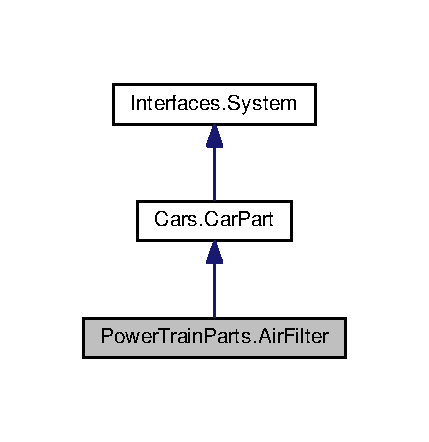
\includegraphics[width=206pt]{classPowerTrainParts_1_1AirFilter__inherit__graph}
\end{center}
\end{figure}


Collaboration diagram for Power\+Train\+Parts.\+Air\+Filter\+:\nopagebreak
\begin{figure}[H]
\begin{center}
\leavevmode
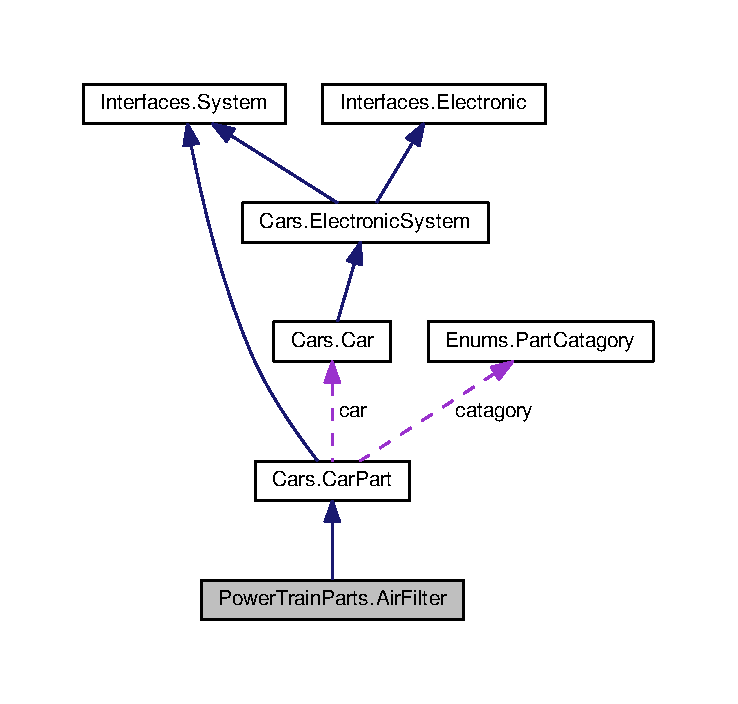
\includegraphics[width=350pt]{classPowerTrainParts_1_1AirFilter__coll__graph}
\end{center}
\end{figure}
\subsection*{Public Member Functions}
\begin{DoxyCompactItemize}
\item 
\hypertarget{classPowerTrainParts_1_1AirFilter_ac3620106d37012faf5c985050aa3db35}{}{\bfseries Air\+Filter} (\hyperlink{classCars_1_1Car}{Car} c, \hyperlink{enumEnums_1_1Location}{Location} loc)\label{classPowerTrainParts_1_1AirFilter_ac3620106d37012faf5c985050aa3db35}

\end{DoxyCompactItemize}
\subsection*{Additional Inherited Members}


The documentation for this class was generated from the following file\+:\begin{DoxyCompactItemize}
\item 
src/\+Power\+Train\+Parts/Air\+Filter.\+java\end{DoxyCompactItemize}

\hypertarget{classElectricalParts_1_1Alternator}{}\section{Electrical\+Parts.\+Alternator Class Reference}
\label{classElectricalParts_1_1Alternator}\index{Electrical\+Parts.\+Alternator@{Electrical\+Parts.\+Alternator}}


Inheritance diagram for Electrical\+Parts.\+Alternator\+:\nopagebreak
\begin{figure}[H]
\begin{center}
\leavevmode
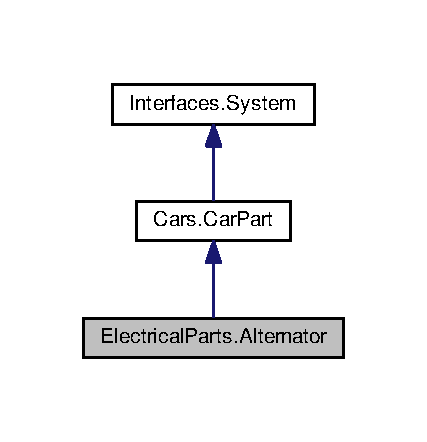
\includegraphics[width=205pt]{classElectricalParts_1_1Alternator__inherit__graph}
\end{center}
\end{figure}


Collaboration diagram for Electrical\+Parts.\+Alternator\+:\nopagebreak
\begin{figure}[H]
\begin{center}
\leavevmode
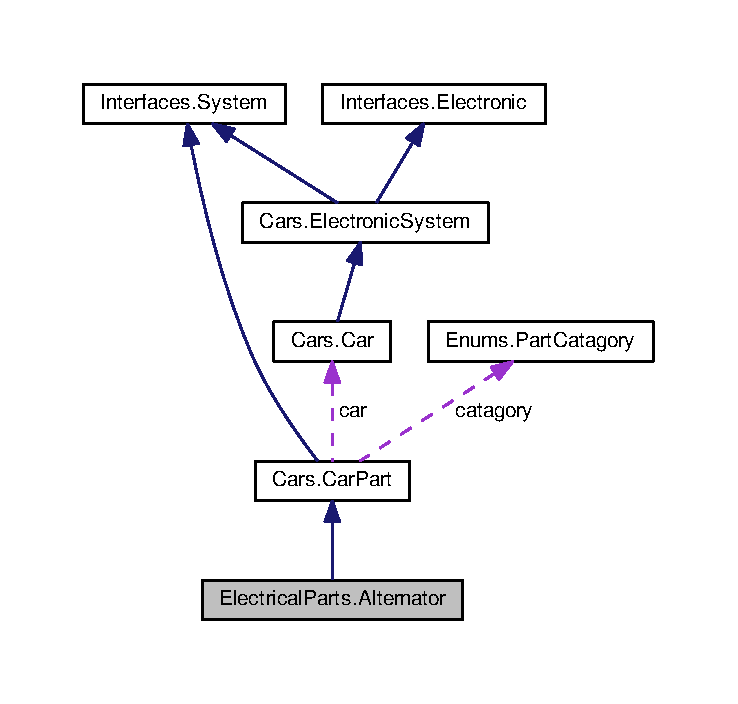
\includegraphics[width=350pt]{classElectricalParts_1_1Alternator__coll__graph}
\end{center}
\end{figure}
\subsection*{Public Member Functions}
\begin{DoxyCompactItemize}
\item 
\hypertarget{classElectricalParts_1_1Alternator_a5ae0780e8c5f063ab85b3bde24c3623b}{}{\bfseries Alternator} (\hyperlink{classCars_1_1Car}{Car} c, \hyperlink{enumEnums_1_1Location}{Location} loc)\label{classElectricalParts_1_1Alternator_a5ae0780e8c5f063ab85b3bde24c3623b}

\item 
\hypertarget{classElectricalParts_1_1Alternator_ad4c99aba0686e4a386d3232884a023c3}{}double {\bfseries power\+Produced} ()\label{classElectricalParts_1_1Alternator_ad4c99aba0686e4a386d3232884a023c3}

\end{DoxyCompactItemize}
\subsection*{Additional Inherited Members}


The documentation for this class was generated from the following file\+:\begin{DoxyCompactItemize}
\item 
src/\+Electrical\+Parts/Alternator.\+java\end{DoxyCompactItemize}

\hypertarget{classElectricalParts_1_1Battery}{}\section{Electrical\+Parts.\+Battery Class Reference}
\label{classElectricalParts_1_1Battery}\index{Electrical\+Parts.\+Battery@{Electrical\+Parts.\+Battery}}


Inheritance diagram for Electrical\+Parts.\+Battery\+:
\nopagebreak
\begin{figure}[H]
\begin{center}
\leavevmode
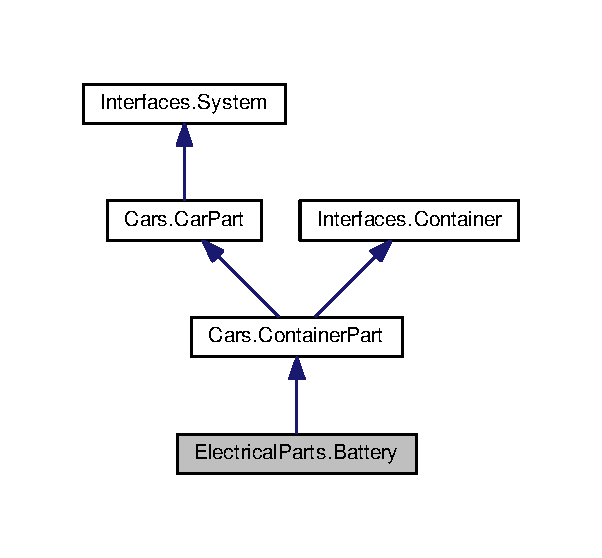
\includegraphics[width=289pt]{classElectricalParts_1_1Battery__inherit__graph}
\end{center}
\end{figure}


Collaboration diagram for Electrical\+Parts.\+Battery\+:
\nopagebreak
\begin{figure}[H]
\begin{center}
\leavevmode
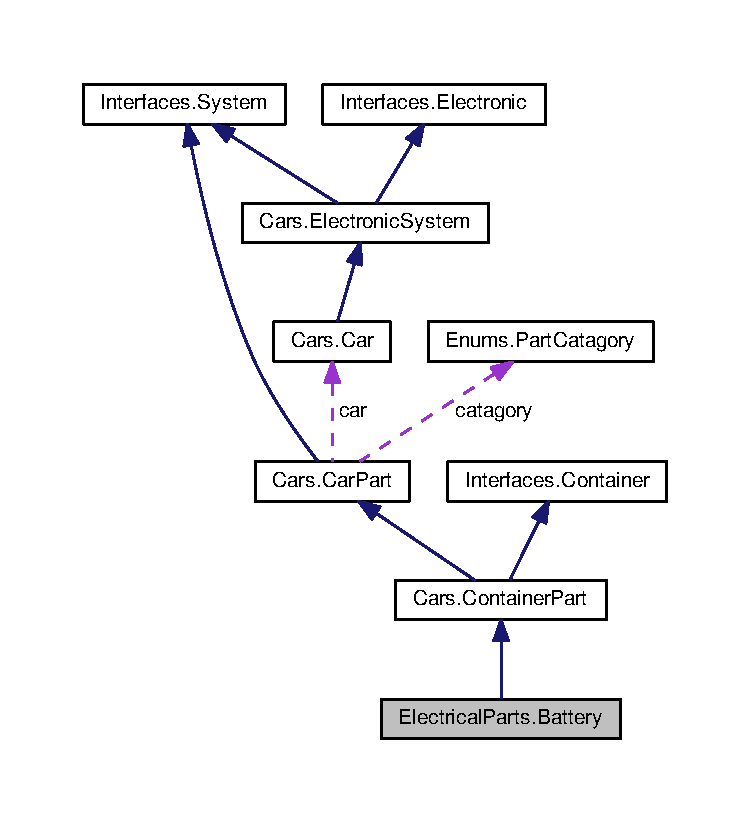
\includegraphics[width=350pt]{classElectricalParts_1_1Battery__coll__graph}
\end{center}
\end{figure}
\subsection*{Public Member Functions}
\begin{DoxyCompactItemize}
\item 
\hypertarget{classElectricalParts_1_1Battery_ae595503240f210b0c2f57098b8c25067}{}boolean {\bfseries operational} ()\label{classElectricalParts_1_1Battery_ae595503240f210b0c2f57098b8c25067}

\item 
\hypertarget{classElectricalParts_1_1Battery_a9e7801530ef808b20252ef73c2d2c96c}{}{\bfseries Battery} (\hyperlink{classCars_1_1Car}{Car} c, \hyperlink{enumEnums_1_1Location}{Location} loc)\label{classElectricalParts_1_1Battery_a9e7801530ef808b20252ef73c2d2c96c}

\item 
\hypertarget{classElectricalParts_1_1Battery_abf3d6f5e7e7b77bbce046f7446a6a879}{}void {\bfseries diagnostic} ()\label{classElectricalParts_1_1Battery_abf3d6f5e7e7b77bbce046f7446a6a879}

\item 
\hypertarget{classElectricalParts_1_1Battery_a132c17ac42aef8470a7f79dde015f9a5}{}void {\bfseries inspect} ()\label{classElectricalParts_1_1Battery_a132c17ac42aef8470a7f79dde015f9a5}

\end{DoxyCompactItemize}
\subsection*{Additional Inherited Members}


The documentation for this class was generated from the following file\+:\begin{DoxyCompactItemize}
\item 
src/\+Electrical\+Parts/Battery.\+java\end{DoxyCompactItemize}

\hypertarget{classSystems_1_1Brakes}{}\section{Systems.\+Brakes Class Reference}
\label{classSystems_1_1Brakes}\index{Systems.\+Brakes@{Systems.\+Brakes}}


Inheritance diagram for Systems.\+Brakes\+:\nopagebreak
\begin{figure}[H]
\begin{center}
\leavevmode
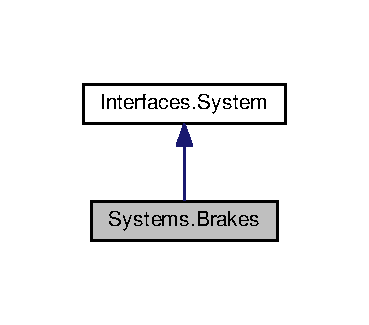
\includegraphics[width=177pt]{classSystems_1_1Brakes__inherit__graph}
\end{center}
\end{figure}


Collaboration diagram for Systems.\+Brakes\+:
\nopagebreak
\begin{figure}[H]
\begin{center}
\leavevmode
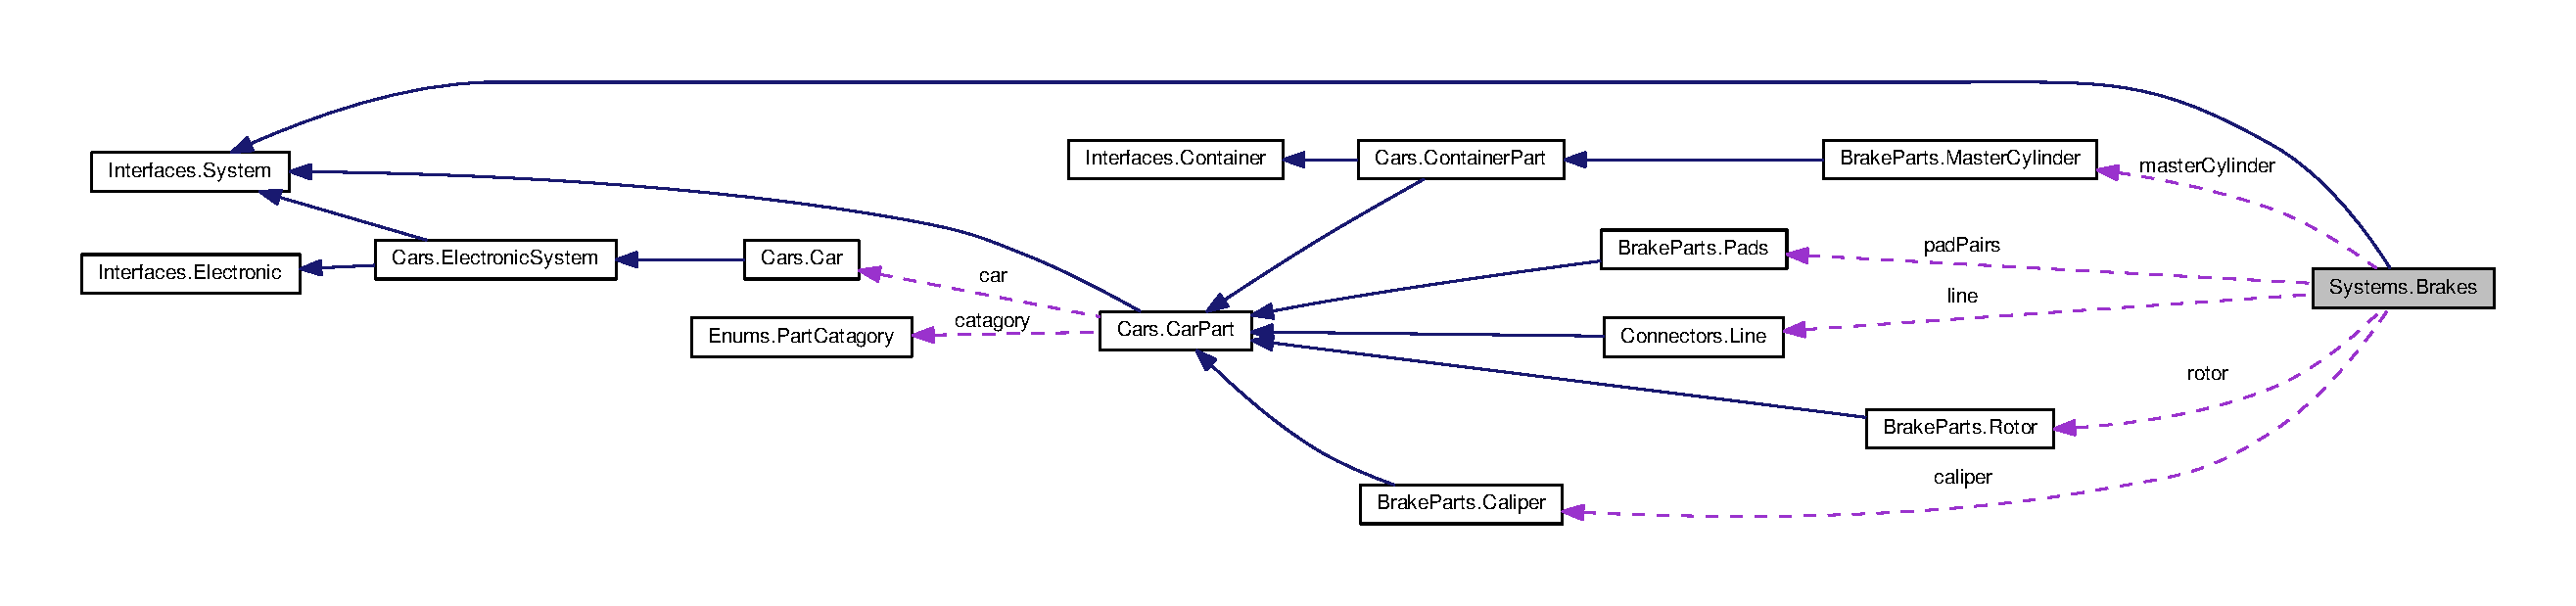
\includegraphics[width=350pt]{classSystems_1_1Brakes__coll__graph}
\end{center}
\end{figure}
\subsection*{Public Member Functions}
\begin{DoxyCompactItemize}
\item 
\hypertarget{classSystems_1_1Brakes_a0417265a254fd287d788b9283f927107}{}{\bfseries Brakes} (\hyperlink{classCars_1_1Car}{Car} car, \hyperlink{enumEnums_1_1Location}{Location} loc)\label{classSystems_1_1Brakes_a0417265a254fd287d788b9283f927107}

\item 
\hypertarget{classSystems_1_1Brakes_a531718d8d1891c18076562bb8e959062}{}boolean {\bfseries operational} ()\label{classSystems_1_1Brakes_a531718d8d1891c18076562bb8e959062}

\item 
\hypertarget{classSystems_1_1Brakes_ab614f7ed7a5ea64ecd07f5a76aeda828}{}boolean {\bfseries replace} (\hyperlink{classCars_1_1CarPart}{Car\+Part} old\+Part, \hyperlink{classCars_1_1CarPart}{Car\+Part} new\+Part)\label{classSystems_1_1Brakes_ab614f7ed7a5ea64ecd07f5a76aeda828}

\item 
\hypertarget{classSystems_1_1Brakes_a9655e179ebec461790cc5567ce48e30d}{}void {\bfseries diagnostic} ()\label{classSystems_1_1Brakes_a9655e179ebec461790cc5567ce48e30d}

\item 
\hypertarget{classSystems_1_1Brakes_ae03579bf1c3bb2ca0d1efde46dd5d7a4}{}void {\bfseries inspect} ()\label{classSystems_1_1Brakes_ae03579bf1c3bb2ca0d1efde46dd5d7a4}

\end{DoxyCompactItemize}


The documentation for this class was generated from the following file\+:\begin{DoxyCompactItemize}
\item 
src/\+Systems/Brakes.\+java\end{DoxyCompactItemize}

\hypertarget{classBrakeParts_1_1Caliper}{}\section{Brake\+Parts.\+Caliper Class Reference}
\label{classBrakeParts_1_1Caliper}\index{Brake\+Parts.\+Caliper@{Brake\+Parts.\+Caliper}}


Inheritance diagram for Brake\+Parts.\+Caliper\+:\nopagebreak
\begin{figure}[H]
\begin{center}
\leavevmode
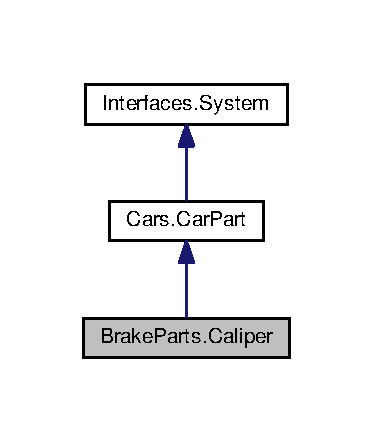
\includegraphics[width=179pt]{classBrakeParts_1_1Caliper__inherit__graph}
\end{center}
\end{figure}


Collaboration diagram for Brake\+Parts.\+Caliper\+:\nopagebreak
\begin{figure}[H]
\begin{center}
\leavevmode
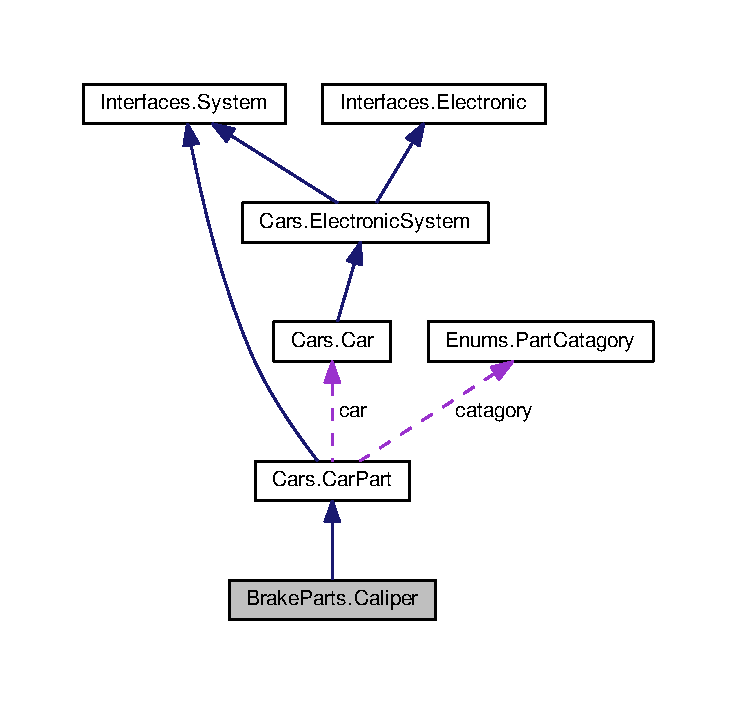
\includegraphics[width=350pt]{classBrakeParts_1_1Caliper__coll__graph}
\end{center}
\end{figure}
\subsection*{Public Member Functions}
\begin{DoxyCompactItemize}
\item 
\hypertarget{classBrakeParts_1_1Caliper_a6b603ed597c11c5cb576d61b3ed8db00}{}{\bfseries Caliper} (\hyperlink{classCars_1_1Car}{Car} c, \hyperlink{enumEnums_1_1Location}{Location} loc)\label{classBrakeParts_1_1Caliper_a6b603ed597c11c5cb576d61b3ed8db00}

\item 
\hypertarget{classBrakeParts_1_1Caliper_a5fda33282ada86c76b46e5407b6e686c}{}boolean {\bfseries operational} ()\label{classBrakeParts_1_1Caliper_a5fda33282ada86c76b46e5407b6e686c}

\end{DoxyCompactItemize}
\subsection*{Additional Inherited Members}


The documentation for this class was generated from the following file\+:\begin{DoxyCompactItemize}
\item 
src/\+Brake\+Parts/Caliper.\+java\end{DoxyCompactItemize}

\hypertarget{classCars_1_1Car}{}\section{Cars.\+Car Class Reference}
\label{classCars_1_1Car}\index{Cars.\+Car@{Cars.\+Car}}


Inheritance diagram for Cars.\+Car\+:\nopagebreak
\begin{figure}[H]
\begin{center}
\leavevmode
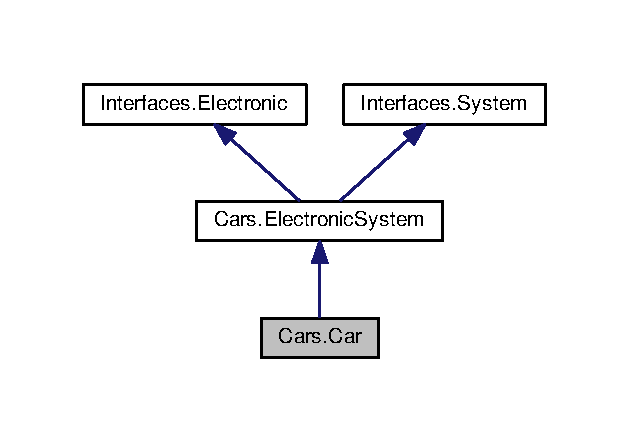
\includegraphics[width=302pt]{classCars_1_1Car__inherit__graph}
\end{center}
\end{figure}


Collaboration diagram for Cars.\+Car\+:\nopagebreak
\begin{figure}[H]
\begin{center}
\leavevmode
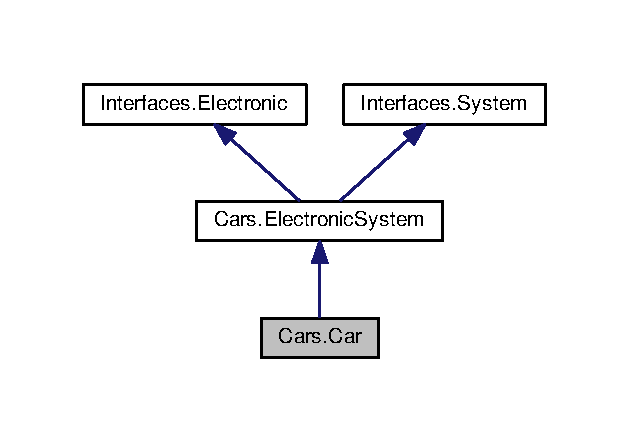
\includegraphics[width=302pt]{classCars_1_1Car__coll__graph}
\end{center}
\end{figure}
\subsection*{Public Member Functions}
\begin{DoxyCompactItemize}
\item 
\hypertarget{classCars_1_1Car_a234016f160ede7f71195720b6c91e660}{}boolean {\bfseries operational} ()\label{classCars_1_1Car_a234016f160ede7f71195720b6c91e660}

\item 
\hypertarget{classCars_1_1Car_aa62627c0bbdcccbb1e09cbd355418804}{}boolean {\bfseries replace} (\hyperlink{classCars_1_1CarPart}{Car\+Part} old\+Part, \hyperlink{classCars_1_1CarPart}{Car\+Part} new\+Part)\label{classCars_1_1Car_aa62627c0bbdcccbb1e09cbd355418804}

\item 
\hypertarget{classCars_1_1Car_acd98adbaa2fa0b328be9ee18e204e671}{}void {\bfseries diagnostic} ()\label{classCars_1_1Car_acd98adbaa2fa0b328be9ee18e204e671}

\item 
\hypertarget{classCars_1_1Car_a06a454f3de50b5681ed1b0b8c29b8b14}{}void {\bfseries inspect} ()\label{classCars_1_1Car_a06a454f3de50b5681ed1b0b8c29b8b14}

\item 
\hypertarget{classCars_1_1Car_a6236a57ea2bfa16888f916d1fe34919f}{}boolean {\bfseries operation\+Loop} ()\label{classCars_1_1Car_a6236a57ea2bfa16888f916d1fe34919f}

\item 
\hypertarget{classCars_1_1Car_ab70985dbffac9c217ec6c7909d7d15af}{}boolean {\bfseries replace\+Part} (\hyperlink{classCars_1_1CarPart}{Car\+Part} old\+Part, \hyperlink{classCars_1_1CarPart}{Car\+Part} new\+Part)\label{classCars_1_1Car_ab70985dbffac9c217ec6c7909d7d15af}

\item 
\hypertarget{classCars_1_1Car_a7ad19523263277304b44f8b0f650ae73}{}synchronized void {\bfseries add\+Hundreth\+Mile} ()\label{classCars_1_1Car_a7ad19523263277304b44f8b0f650ae73}

\item 
\hypertarget{classCars_1_1Car_a7bf8ab93d4c9e2bd7dbf9ce24dedae24}{}synchronized int {\bfseries get\+Miles} ()\label{classCars_1_1Car_a7bf8ab93d4c9e2bd7dbf9ce24dedae24}

\item 
\hypertarget{classCars_1_1Car_a09079918be69fcad4da0bf9c02331bad}{}\hyperlink{classSystems_1_1Brakes}{Brakes} {\bfseries get\+Brakes} ()\label{classCars_1_1Car_a09079918be69fcad4da0bf9c02331bad}

\item 
\hypertarget{classCars_1_1Car_a63da80c1f2c1972df0a7fb2d35ad5c73}{}\hyperlink{classSystems_1_1DriveTrain}{Drive\+Train} {\bfseries get\+Drive\+Train} ()\label{classCars_1_1Car_a63da80c1f2c1972df0a7fb2d35ad5c73}

\item 
\hypertarget{classCars_1_1Car_a9f309a7c774d62c23e2e44f4e46be455}{}\hyperlink{classSystems_1_1Ignition}{Ignition} {\bfseries get\+Ignition} ()\label{classCars_1_1Car_a9f309a7c774d62c23e2e44f4e46be455}

\item 
\hypertarget{classCars_1_1Car_afe1f29ceb135766ab588499f02265a80}{}\hyperlink{classSystems_1_1Fuel}{Fuel} {\bfseries get\+Fuel} ()\label{classCars_1_1Car_afe1f29ceb135766ab588499f02265a80}

\item 
\hypertarget{classCars_1_1Car_ab78bd960acb494443728b1c945976e09}{}\hyperlink{classSystems_1_1Electrical}{Electrical} {\bfseries get\+Electrical} ()\label{classCars_1_1Car_ab78bd960acb494443728b1c945976e09}

\item 
\hypertarget{classCars_1_1Car_a0584fce677654c11e1c229a310b183dc}{}\hyperlink{classSystems_1_1PowerTrain}{Power\+Train} {\bfseries get\+Power\+Train} ()\label{classCars_1_1Car_a0584fce677654c11e1c229a310b183dc}

\item 
\hypertarget{classCars_1_1Car_aa4c9b12767c3f2e3d40e05803065b0c1}{}\hyperlink{classSystems_1_1Suspension}{Suspension} {\bfseries get\+Suspension} ()\label{classCars_1_1Car_aa4c9b12767c3f2e3d40e05803065b0c1}

\item 
\hypertarget{classCars_1_1Car_a4173d3ecdf52118ba6b450efee2b5084}{}\hyperlink{classIgnitionParts_1_1Starter}{Starter} {\bfseries get\+Starter} ()\label{classCars_1_1Car_a4173d3ecdf52118ba6b450efee2b5084}

\item 
\hypertarget{classCars_1_1Car_a7fe1d8b3916b2205eeb36f585a3f3f29}{}\hyperlink{classPowerTrainParts_1_1Motor}{Motor} {\bfseries get\+Motor} ()\label{classCars_1_1Car_a7fe1d8b3916b2205eeb36f585a3f3f29}

\item 
\hypertarget{classCars_1_1Car_aaef37aabdc5d1ded793fa8156dcba4d7}{}\hyperlink{classBrakeParts_1_1MasterCylinder}{Master\+Cylinder} {\bfseries get\+Mas\+Cyl} ()\label{classCars_1_1Car_aaef37aabdc5d1ded793fa8156dcba4d7}

\item 
\hypertarget{classCars_1_1Car_a9548527677ae80277715ab599a0c1c54}{}\hyperlink{classElectricalParts_1_1Battery}{Battery} {\bfseries get\+Battery} ()\label{classCars_1_1Car_a9548527677ae80277715ab599a0c1c54}

\item 
\hypertarget{classCars_1_1Car_aaa049b1e0983825e398e33bcbe177949}{}\hyperlink{classFuelSystemParts_1_1Tank}{Tank} {\bfseries get\+Tank} ()\label{classCars_1_1Car_aaa049b1e0983825e398e33bcbe177949}

\end{DoxyCompactItemize}
\subsection*{Additional Inherited Members}


The documentation for this class was generated from the following file\+:\begin{DoxyCompactItemize}
\item 
src/\+Cars/Car.\+java\end{DoxyCompactItemize}

\hypertarget{classCars_1_1CarPart}{}\section{Cars.\+Car\+Part Class Reference}
\label{classCars_1_1CarPart}\index{Cars.\+Car\+Part@{Cars.\+Car\+Part}}


Inheritance diagram for Cars.\+Car\+Part\+:\nopagebreak
\begin{figure}[H]
\begin{center}
\leavevmode
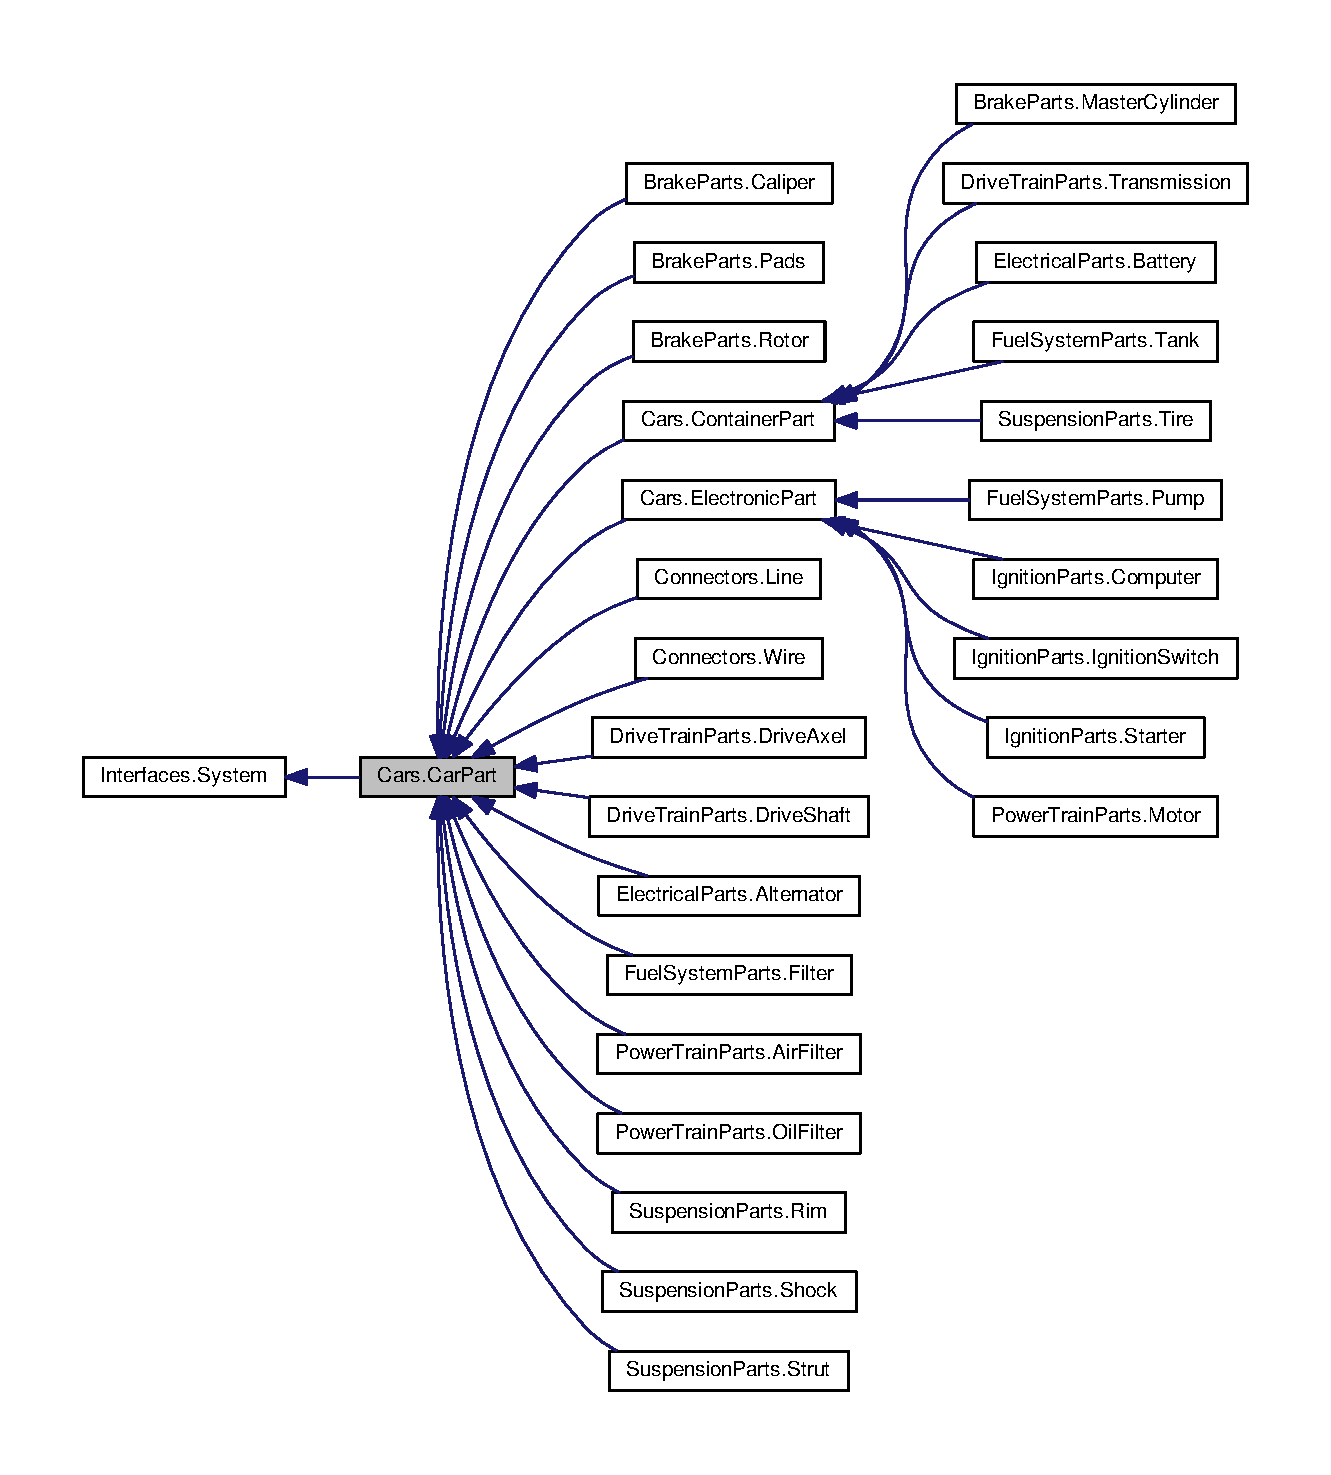
\includegraphics[width=350pt]{classCars_1_1CarPart__inherit__graph}
\end{center}
\end{figure}


Collaboration diagram for Cars.\+Car\+Part\+:\nopagebreak
\begin{figure}[H]
\begin{center}
\leavevmode
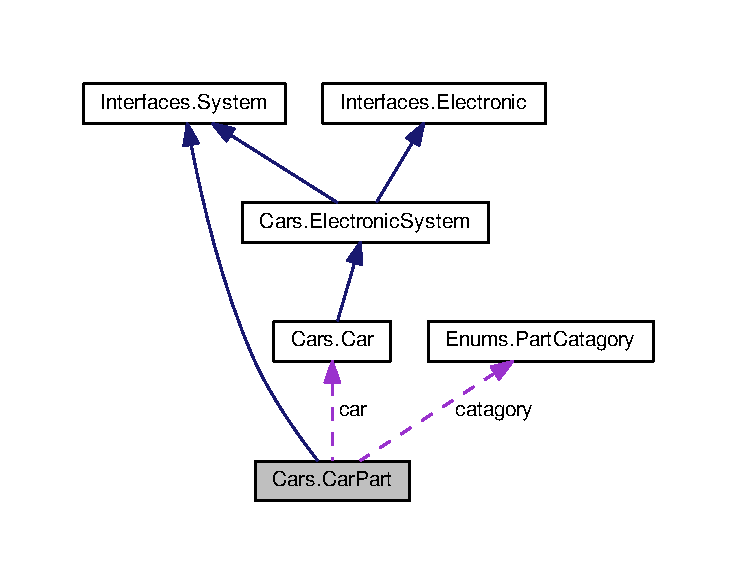
\includegraphics[width=350pt]{classCars_1_1CarPart__coll__graph}
\end{center}
\end{figure}
\subsection*{Public Member Functions}
\begin{DoxyCompactItemize}
\item 
\hypertarget{classCars_1_1CarPart_acec30c01ebd3b7101b58134eda02a82c}{}boolean {\bfseries replace} (\hyperlink{classCars_1_1CarPart}{Car\+Part} old\+Part, \hyperlink{classCars_1_1CarPart}{Car\+Part} new\+Part)\label{classCars_1_1CarPart_acec30c01ebd3b7101b58134eda02a82c}

\item 
\hypertarget{classCars_1_1CarPart_a0a01ef76cb96674327f5709fa03a7ee7}{}\hyperlink{enumEnums_1_1Location}{Location} {\bfseries get\+Location} ()\label{classCars_1_1CarPart_a0a01ef76cb96674327f5709fa03a7ee7}

\item 
\hypertarget{classCars_1_1CarPart_aa042bb8f4a02ad6964bd70f1cc1a9c16}{}\hyperlink{enumEnums_1_1Status}{Status} {\bfseries get\+Status} ()\label{classCars_1_1CarPart_aa042bb8f4a02ad6964bd70f1cc1a9c16}

\item 
\hypertarget{classCars_1_1CarPart_a333807040e31fa3bdc186b21bbfbd219}{}void {\bfseries inspect} ()\label{classCars_1_1CarPart_a333807040e31fa3bdc186b21bbfbd219}

\item 
\hypertarget{classCars_1_1CarPart_a5dd0c890afe18965762a7a5c28c0bf4e}{}void {\bfseries diagnostic} ()\label{classCars_1_1CarPart_a5dd0c890afe18965762a7a5c28c0bf4e}

\item 
\hypertarget{classCars_1_1CarPart_a3aa4a7e089dd39c43e758b48a0f5f4fd}{}boolean {\bfseries operational} ()\label{classCars_1_1CarPart_a3aa4a7e089dd39c43e758b48a0f5f4fd}

\item 
\hypertarget{classCars_1_1CarPart_adf156fb8effd8e0d65704f61f90237d0}{}void {\bfseries life\+Time\+Status} ()\label{classCars_1_1CarPart_adf156fb8effd8e0d65704f61f90237d0}

\item 
\hypertarget{classCars_1_1CarPart_af8ff7d6936131b58164ba61ce26cd6b4}{}double {\bfseries get\+Weight} ()\label{classCars_1_1CarPart_af8ff7d6936131b58164ba61ce26cd6b4}

\item 
\hypertarget{classCars_1_1CarPart_ad3be05c274c4865eec7e376db6886670}{}\hyperlink{classCars_1_1Car}{Car} {\bfseries get\+Car} ()\label{classCars_1_1CarPart_ad3be05c274c4865eec7e376db6886670}

\item 
\hypertarget{classCars_1_1CarPart_a44e81419b449a6d179a898e7848dfe9d}{}void {\bfseries set\+Car} (\hyperlink{classCars_1_1Car}{Car} car)\label{classCars_1_1CarPart_a44e81419b449a6d179a898e7848dfe9d}

\item 
\hypertarget{classCars_1_1CarPart_afe58883ee1a34c15dc47b27598805440}{}String {\bfseries get\+Part\+Name} ()\label{classCars_1_1CarPart_afe58883ee1a34c15dc47b27598805440}

\item 
\hypertarget{classCars_1_1CarPart_a0f2d54945d30bf9c81d37746a41a803b}{}String {\bfseries get\+Part\+Number} ()\label{classCars_1_1CarPart_a0f2d54945d30bf9c81d37746a41a803b}

\item 
\hypertarget{classCars_1_1CarPart_aff2dc5a2b1e54e9ee4dec506ec5dc406}{}int {\bfseries get\+Last\+Inspection} ()\label{classCars_1_1CarPart_aff2dc5a2b1e54e9ee4dec506ec5dc406}

\item 
\hypertarget{classCars_1_1CarPart_aad97e59cbf9ce5b5663298c8146c2eb9}{}void {\bfseries break\+Part} ()\label{classCars_1_1CarPart_aad97e59cbf9ce5b5663298c8146c2eb9}

\item 
\hypertarget{classCars_1_1CarPart_af211157f3b4eeb3f53ca3827597aae4b}{}\hyperlink{enumEnums_1_1PartCatagory}{Part\+Catagory} {\bfseries get\+Catagory} ()\label{classCars_1_1CarPart_af211157f3b4eeb3f53ca3827597aae4b}

\item 
\hypertarget{classCars_1_1CarPart_a69b322ca1b091cf9e957e85219d18d7e}{}void {\bfseries set\+Catagory} (\hyperlink{enumEnums_1_1PartCatagory}{Part\+Catagory} catagory)\label{classCars_1_1CarPart_a69b322ca1b091cf9e957e85219d18d7e}

\item 
\hypertarget{classCars_1_1CarPart_ae82366176fa4fd700b84a6e6fd84d9ba}{}void {\bfseries set\+Location} (\hyperlink{enumEnums_1_1Location}{Location} location)\label{classCars_1_1CarPart_ae82366176fa4fd700b84a6e6fd84d9ba}

\item 
\hypertarget{classCars_1_1CarPart_a9cdf481fa5558112c93a7a05b7a2c046}{}void {\bfseries print\+Part\+Error} (String error)\label{classCars_1_1CarPart_a9cdf481fa5558112c93a7a05b7a2c046}

\end{DoxyCompactItemize}
\subsection*{Static Public Member Functions}
\begin{DoxyCompactItemize}
\item 
\hypertarget{classCars_1_1CarPart_aa99ded7306f0a2e9efe0ffee86d8dc36}{}static void {\bfseries inspect} (\hyperlink{classCars_1_1CarPart}{Car\+Part} cp, String part\+Name)\label{classCars_1_1CarPart_aa99ded7306f0a2e9efe0ffee86d8dc36}

\item 
\hypertarget{classCars_1_1CarPart_a076adbc952554a628b9351814ec12285}{}static void {\bfseries print\+No\+Data} ()\label{classCars_1_1CarPart_a076adbc952554a628b9351814ec12285}

\end{DoxyCompactItemize}
\subsection*{Protected Member Functions}
\begin{DoxyCompactItemize}
\item 
\hypertarget{classCars_1_1CarPart_a46569fe9c033ec91ee0b31874460527a}{}void {\bfseries initialize} (\hyperlink{classCars_1_1Car}{Car} c, \hyperlink{enumEnums_1_1PartCatagory}{Part\+Catagory} cat, double wgt, String pname, String pnum, \hyperlink{enumEnums_1_1Location}{Location} l)\label{classCars_1_1CarPart_a46569fe9c033ec91ee0b31874460527a}

\end{DoxyCompactItemize}
\subsection*{Protected Attributes}
\begin{DoxyCompactItemize}
\item 
\hypertarget{classCars_1_1CarPart_a34325cfedc4e5edda4c03c8c96f85a98}{}\hyperlink{enumEnums_1_1PartCatagory}{Part\+Catagory} {\bfseries catagory}\label{classCars_1_1CarPart_a34325cfedc4e5edda4c03c8c96f85a98}

\item 
\hypertarget{classCars_1_1CarPart_a6cc9b41d99cf9ae855f44b3295384e56}{}\hyperlink{classCars_1_1Car}{Car} {\bfseries car}\label{classCars_1_1CarPart_a6cc9b41d99cf9ae855f44b3295384e56}

\item 
\hypertarget{classCars_1_1CarPart_a6d52f6a89059a44d113fa63e5169b3fc}{}double {\bfseries weight}\label{classCars_1_1CarPart_a6d52f6a89059a44d113fa63e5169b3fc}

\end{DoxyCompactItemize}


The documentation for this class was generated from the following file\+:\begin{DoxyCompactItemize}
\item 
src/\+Cars/Car\+Part.\+java\end{DoxyCompactItemize}

\hypertarget{classCars_1_1CarPartVector}{}\section{Cars.\+Car\+Part\+Vector Class Reference}
\label{classCars_1_1CarPartVector}\index{Cars.\+Car\+Part\+Vector@{Cars.\+Car\+Part\+Vector}}


Inheritance diagram for Cars.\+Car\+Part\+Vector\+:\nopagebreak
\begin{figure}[H]
\begin{center}
\leavevmode
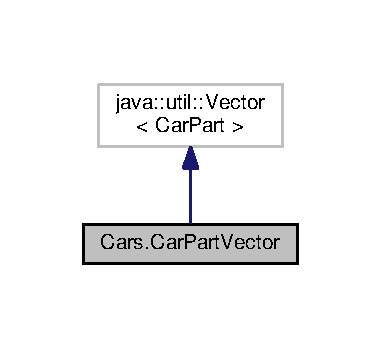
\includegraphics[width=183pt]{classCars_1_1CarPartVector__inherit__graph}
\end{center}
\end{figure}


Collaboration diagram for Cars.\+Car\+Part\+Vector\+:\nopagebreak
\begin{figure}[H]
\begin{center}
\leavevmode
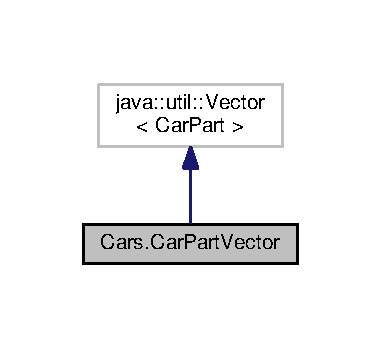
\includegraphics[width=183pt]{classCars_1_1CarPartVector__coll__graph}
\end{center}
\end{figure}
\subsection*{Public Member Functions}
\begin{DoxyCompactItemize}
\item 
\hypertarget{classCars_1_1CarPartVector_a1c6a5a8d049ecb65a8d0112f9270f429}{}boolean {\bfseries replace} (\hyperlink{classCars_1_1CarPart}{Car\+Part} ele\+Old, \hyperlink{classCars_1_1CarPart}{Car\+Part} ele\+New)\label{classCars_1_1CarPartVector_a1c6a5a8d049ecb65a8d0112f9270f429}

\item 
\hypertarget{classCars_1_1CarPartVector_ad4aecfdfc302dd502a626b594d0a1697}{}void {\bfseries inspect\+All} ()\label{classCars_1_1CarPartVector_ad4aecfdfc302dd502a626b594d0a1697}

\item 
\hypertarget{classCars_1_1CarPartVector_a8a65c1c7f791193517f72d4da8cf5f9d}{}boolean {\bfseries all\+Operational} ()\label{classCars_1_1CarPartVector_a8a65c1c7f791193517f72d4da8cf5f9d}

\item 
\hypertarget{classCars_1_1CarPartVector_a1cb6cfda741e40c2ad33258ffb6faa38}{}boolean {\bfseries one\+Operational} ()\label{classCars_1_1CarPartVector_a1cb6cfda741e40c2ad33258ffb6faa38}

\item 
\hypertarget{classCars_1_1CarPartVector_a1aca5e2021f13ef5a15610f16f1a857e}{}boolean {\bfseries find\+Locations} (Vector$<$ \hyperlink{enumEnums_1_1Location}{Enums.\+Location} $>$ locations)\label{classCars_1_1CarPartVector_a1aca5e2021f13ef5a15610f16f1a857e}

\item 
\hypertarget{classCars_1_1CarPartVector_a202b162ca9cf3a19128c9e210c8f00bb}{}void {\bfseries create} (String class\+Name, Vector$<$ \hyperlink{enumEnums_1_1Location}{Enums.\+Location} $>$ locations, \hyperlink{interfaceInterfaces_1_1Iterative}{Iterative} it)\label{classCars_1_1CarPartVector_a202b162ca9cf3a19128c9e210c8f00bb}

\end{DoxyCompactItemize}
\subsection*{Static Public Member Functions}
\begin{DoxyCompactItemize}
\item 
\hypertarget{classCars_1_1CarPartVector_ab8a03fc8aa2b833c3adcf0b046333bed}{}static \hyperlink{classCars_1_1CarPartVector}{Car\+Part\+Vector} {\bfseries convert} (Vector$<$ \hyperlink{classCars_1_1CarPart}{Car\+Part} $>$ vcp)\label{classCars_1_1CarPartVector_ab8a03fc8aa2b833c3adcf0b046333bed}

\end{DoxyCompactItemize}


The documentation for this class was generated from the following file\+:\begin{DoxyCompactItemize}
\item 
src/\+Cars/Car\+Part\+Vector.\+java\end{DoxyCompactItemize}

\hypertarget{classIgnitionParts_1_1Computer}{}\section{Ignition\+Parts.\+Computer Class Reference}
\label{classIgnitionParts_1_1Computer}\index{Ignition\+Parts.\+Computer@{Ignition\+Parts.\+Computer}}


Inheritance diagram for Ignition\+Parts.\+Computer\+:\nopagebreak
\begin{figure}[H]
\begin{center}
\leavevmode
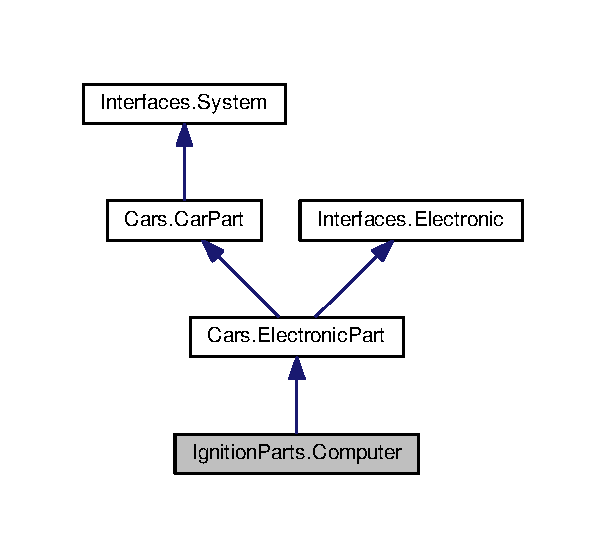
\includegraphics[width=291pt]{classIgnitionParts_1_1Computer__inherit__graph}
\end{center}
\end{figure}


Collaboration diagram for Ignition\+Parts.\+Computer\+:\nopagebreak
\begin{figure}[H]
\begin{center}
\leavevmode
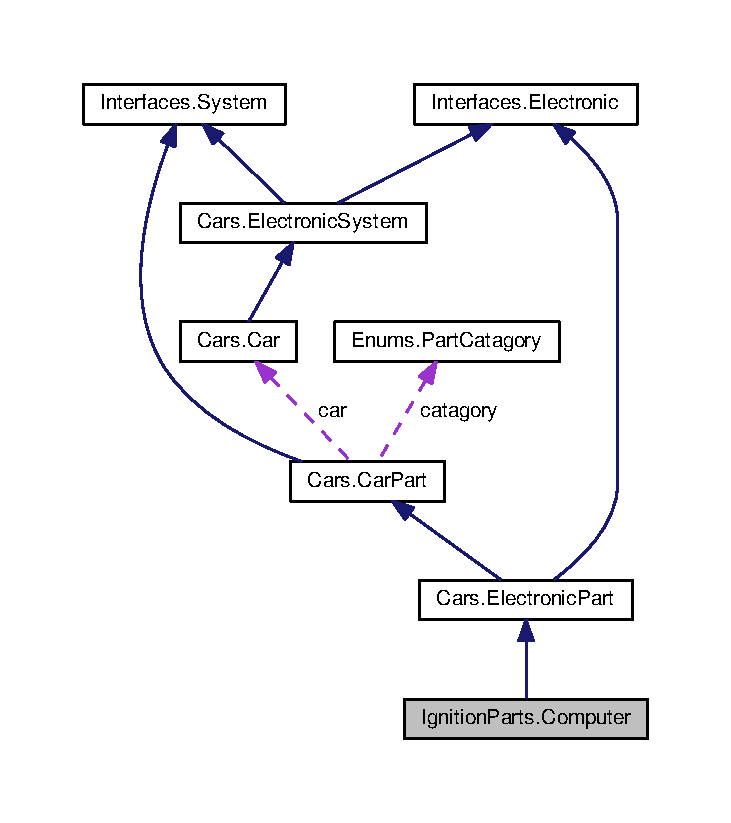
\includegraphics[width=350pt]{classIgnitionParts_1_1Computer__coll__graph}
\end{center}
\end{figure}
\subsection*{Public Member Functions}
\begin{DoxyCompactItemize}
\item 
\hypertarget{classIgnitionParts_1_1Computer_a491a5adfba04ac4ba724bab627565d52}{}{\bfseries Computer} (\hyperlink{classCars_1_1Car}{Car} c, \hyperlink{enumEnums_1_1Location}{Location} loc)\label{classIgnitionParts_1_1Computer_a491a5adfba04ac4ba724bab627565d52}

\item 
\hypertarget{classIgnitionParts_1_1Computer_aafdc32452550624dc8c72b3c17868cc9}{}boolean {\bfseries operational} ()\label{classIgnitionParts_1_1Computer_aafdc32452550624dc8c72b3c17868cc9}

\item 
\hypertarget{classIgnitionParts_1_1Computer_a73944eafa798c9bf232d6e7a3c9f9b3f}{}boolean {\bfseries operation\+Loop} ()\label{classIgnitionParts_1_1Computer_a73944eafa798c9bf232d6e7a3c9f9b3f}

\end{DoxyCompactItemize}
\subsection*{Additional Inherited Members}


The documentation for this class was generated from the following file\+:\begin{DoxyCompactItemize}
\item 
src/\+Ignition\+Parts/Computer.\+java\end{DoxyCompactItemize}

\hypertarget{interfaceInterfaces_1_1Container}{}\section{Interfaces.\+Container Interface Reference}
\label{interfaceInterfaces_1_1Container}\index{Interfaces.\+Container@{Interfaces.\+Container}}


Inheritance diagram for Interfaces.\+Container\+:
\nopagebreak
\begin{figure}[H]
\begin{center}
\leavevmode
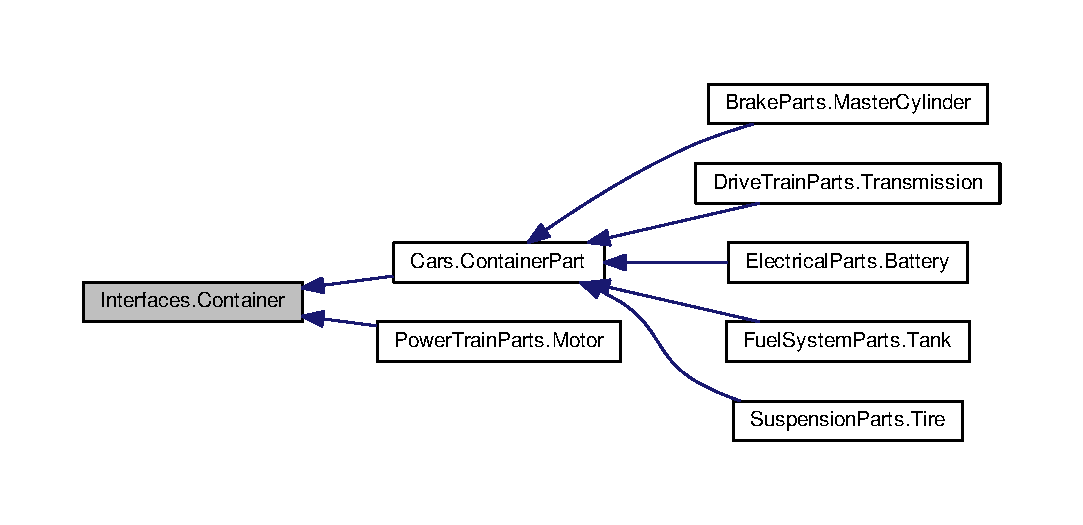
\includegraphics[width=350pt]{interfaceInterfaces_1_1Container__inherit__graph}
\end{center}
\end{figure}
\subsection*{Public Member Functions}
\begin{DoxyCompactItemize}
\item 
\hypertarget{interfaceInterfaces_1_1Container_ac8ce4ee17f9add47e4b292451796eb0b}{}String {\bfseries check\+Level} ()\label{interfaceInterfaces_1_1Container_ac8ce4ee17f9add47e4b292451796eb0b}

\item 
\hypertarget{interfaceInterfaces_1_1Container_a96bed856ca707af69e01a1fc30fc24c4}{}double {\bfseries get\+Capacity} ()\label{interfaceInterfaces_1_1Container_a96bed856ca707af69e01a1fc30fc24c4}

\item 
\hypertarget{interfaceInterfaces_1_1Container_ac5211049926460d75c3adb0c577ee02b}{}void {\bfseries top\+Off} ()\label{interfaceInterfaces_1_1Container_ac5211049926460d75c3adb0c577ee02b}

\item 
\hypertarget{interfaceInterfaces_1_1Container_a99f4519821f22ff8da5d5f329300c622}{}void {\bfseries replace\+Contents} ()\label{interfaceInterfaces_1_1Container_a99f4519821f22ff8da5d5f329300c622}

\item 
\hypertarget{interfaceInterfaces_1_1Container_a1750d47ec1880c6fc2f1296a9d79a372}{}double {\bfseries get\+Last\+Flush} ()\label{interfaceInterfaces_1_1Container_a1750d47ec1880c6fc2f1296a9d79a372}

\end{DoxyCompactItemize}


The documentation for this interface was generated from the following file\+:\begin{DoxyCompactItemize}
\item 
src/\+Interfaces/Container.\+java\end{DoxyCompactItemize}

\hypertarget{classCars_1_1ContainerPart}{}\section{Cars.\+Container\+Part Class Reference}
\label{classCars_1_1ContainerPart}\index{Cars.\+Container\+Part@{Cars.\+Container\+Part}}


Inheritance diagram for Cars.\+Container\+Part\+:
\nopagebreak
\begin{figure}[H]
\begin{center}
\leavevmode
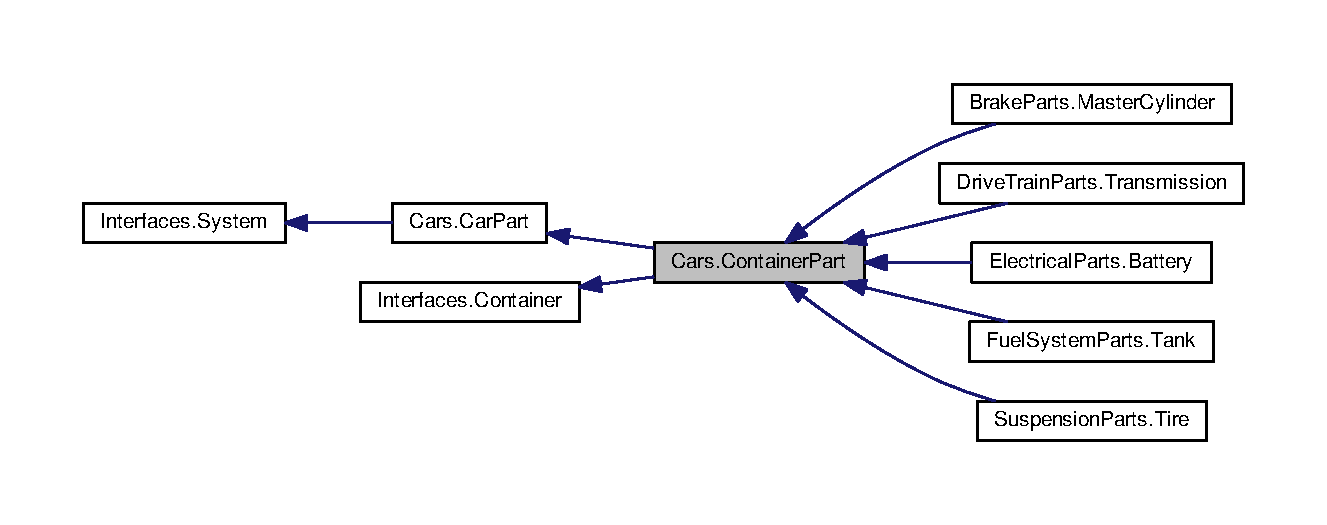
\includegraphics[width=350pt]{classCars_1_1ContainerPart__inherit__graph}
\end{center}
\end{figure}


Collaboration diagram for Cars.\+Container\+Part\+:
\nopagebreak
\begin{figure}[H]
\begin{center}
\leavevmode
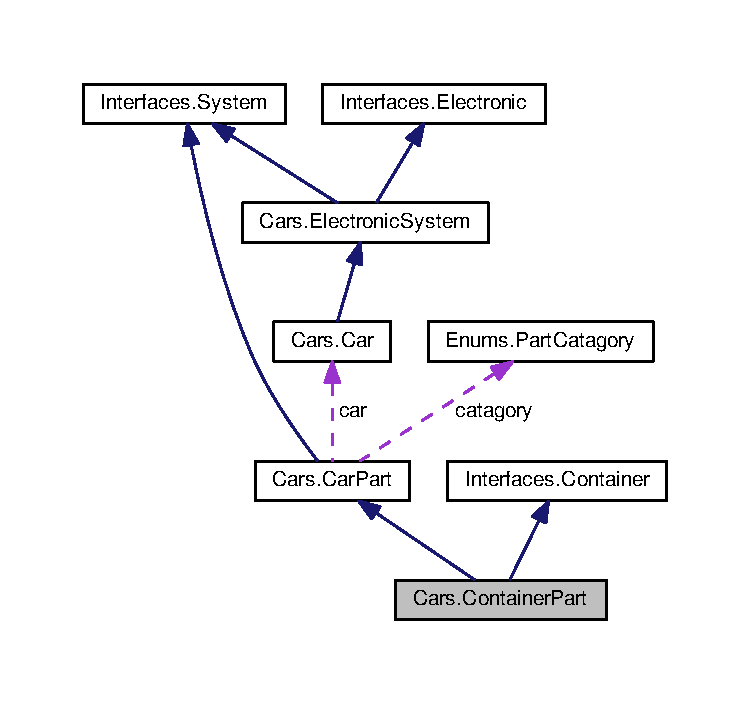
\includegraphics[width=350pt]{classCars_1_1ContainerPart__coll__graph}
\end{center}
\end{figure}
\subsection*{Public Member Functions}
\begin{DoxyCompactItemize}
\item 
\hypertarget{classCars_1_1ContainerPart_aee6d47b18bd47d9d0ae3df15850d8ef0}{}synchronized void {\bfseries charge} (double val)\label{classCars_1_1ContainerPart_aee6d47b18bd47d9d0ae3df15850d8ef0}

\item 
\hypertarget{classCars_1_1ContainerPart_a336bd533d055d4b00a8b9d9c95efbc04}{}synchronized boolean {\bfseries drain} (double val)\label{classCars_1_1ContainerPart_a336bd533d055d4b00a8b9d9c95efbc04}

\item 
\hypertarget{classCars_1_1ContainerPart_ad1c5e9148925a436030bebe633e853f6}{}String {\bfseries check\+Level} ()\label{classCars_1_1ContainerPart_ad1c5e9148925a436030bebe633e853f6}

\item 
\hypertarget{classCars_1_1ContainerPart_a21a9469aedf362d4e77e2a4d4fa4333f}{}double {\bfseries get\+Percent} ()\label{classCars_1_1ContainerPart_a21a9469aedf362d4e77e2a4d4fa4333f}

\item 
\hypertarget{classCars_1_1ContainerPart_a16cfca5c5cc7e094fea194d66d15ce96}{}double {\bfseries get\+Capacity} ()\label{classCars_1_1ContainerPart_a16cfca5c5cc7e094fea194d66d15ce96}

\item 
\hypertarget{classCars_1_1ContainerPart_abb73374ab7b33c860c8a6da853f69cdd}{}void {\bfseries top\+Off} ()\label{classCars_1_1ContainerPart_abb73374ab7b33c860c8a6da853f69cdd}

\item 
\hypertarget{classCars_1_1ContainerPart_a6d9dc65ef1b5c949e520291701b6b632}{}void {\bfseries replace\+Contents} ()\label{classCars_1_1ContainerPart_a6d9dc65ef1b5c949e520291701b6b632}

\item 
\hypertarget{classCars_1_1ContainerPart_aa75f39e4ed5153272e1b878c3050e7a6}{}double {\bfseries get\+Last\+Flush} ()\label{classCars_1_1ContainerPart_aa75f39e4ed5153272e1b878c3050e7a6}

\end{DoxyCompactItemize}
\subsection*{Protected Member Functions}
\begin{DoxyCompactItemize}
\item 
\hypertarget{classCars_1_1ContainerPart_a8ddc2f1fb791c2ed0a55d0cd8e1f10fc}{}void {\bfseries initialize} (double l, double c, double t, double fa)\label{classCars_1_1ContainerPart_a8ddc2f1fb791c2ed0a55d0cd8e1f10fc}

\end{DoxyCompactItemize}
\subsection*{Additional Inherited Members}


The documentation for this class was generated from the following file\+:\begin{DoxyCompactItemize}
\item 
src/\+Cars/Container\+Part.\+java\end{DoxyCompactItemize}

\hypertarget{classDriveTrainParts_1_1DriveAxel}{}\section{Drive\+Train\+Parts.\+Drive\+Axel Class Reference}
\label{classDriveTrainParts_1_1DriveAxel}\index{Drive\+Train\+Parts.\+Drive\+Axel@{Drive\+Train\+Parts.\+Drive\+Axel}}


Inheritance diagram for Drive\+Train\+Parts.\+Drive\+Axel\+:\nopagebreak
\begin{figure}[H]
\begin{center}
\leavevmode
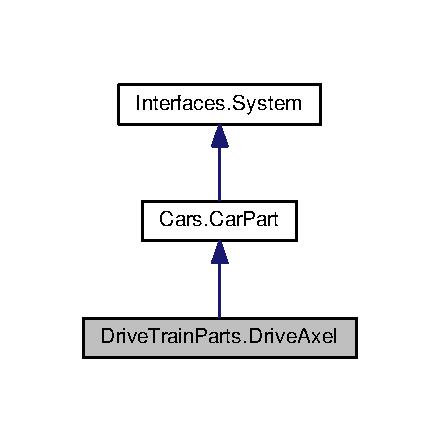
\includegraphics[width=211pt]{classDriveTrainParts_1_1DriveAxel__inherit__graph}
\end{center}
\end{figure}


Collaboration diagram for Drive\+Train\+Parts.\+Drive\+Axel\+:\nopagebreak
\begin{figure}[H]
\begin{center}
\leavevmode
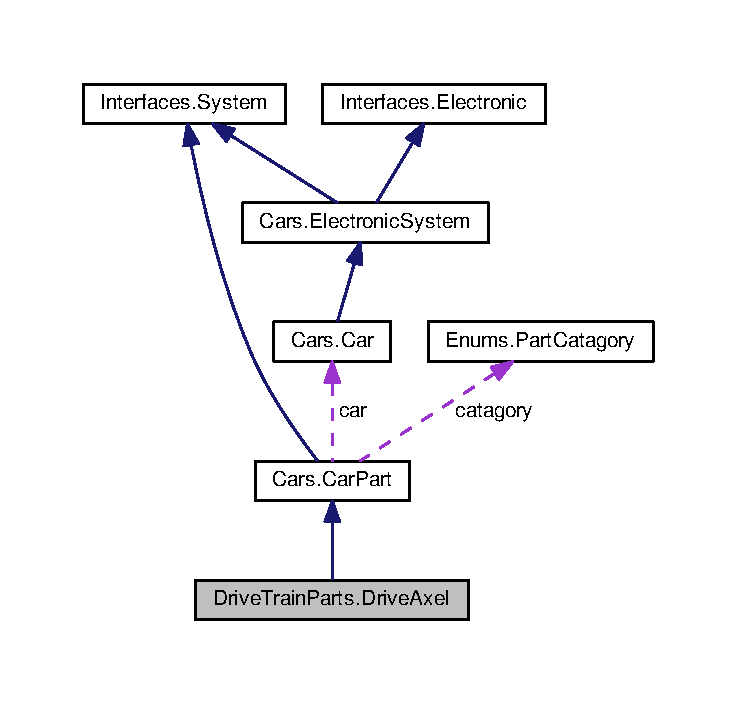
\includegraphics[width=350pt]{classDriveTrainParts_1_1DriveAxel__coll__graph}
\end{center}
\end{figure}
\subsection*{Public Member Functions}
\begin{DoxyCompactItemize}
\item 
\hypertarget{classDriveTrainParts_1_1DriveAxel_a10144004573000625364f2d4cc39b954}{}{\bfseries Drive\+Axel} (\hyperlink{classCars_1_1Car}{Car} c, \hyperlink{enumEnums_1_1Location}{Location} loc)\label{classDriveTrainParts_1_1DriveAxel_a10144004573000625364f2d4cc39b954}

\end{DoxyCompactItemize}
\subsection*{Additional Inherited Members}


The documentation for this class was generated from the following file\+:\begin{DoxyCompactItemize}
\item 
src/\+Drive\+Train\+Parts/Drive\+Axel.\+java\end{DoxyCompactItemize}

\hypertarget{classDriveTrainParts_1_1DriveShaft}{}\section{Drive\+Train\+Parts.\+Drive\+Shaft Class Reference}
\label{classDriveTrainParts_1_1DriveShaft}\index{Drive\+Train\+Parts.\+Drive\+Shaft@{Drive\+Train\+Parts.\+Drive\+Shaft}}


Inheritance diagram for Drive\+Train\+Parts.\+Drive\+Shaft\+:\nopagebreak
\begin{figure}[H]
\begin{center}
\leavevmode
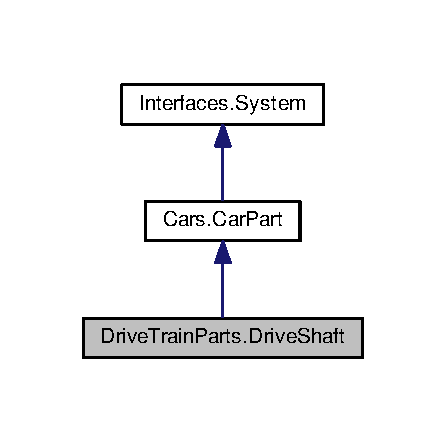
\includegraphics[width=214pt]{classDriveTrainParts_1_1DriveShaft__inherit__graph}
\end{center}
\end{figure}


Collaboration diagram for Drive\+Train\+Parts.\+Drive\+Shaft\+:\nopagebreak
\begin{figure}[H]
\begin{center}
\leavevmode
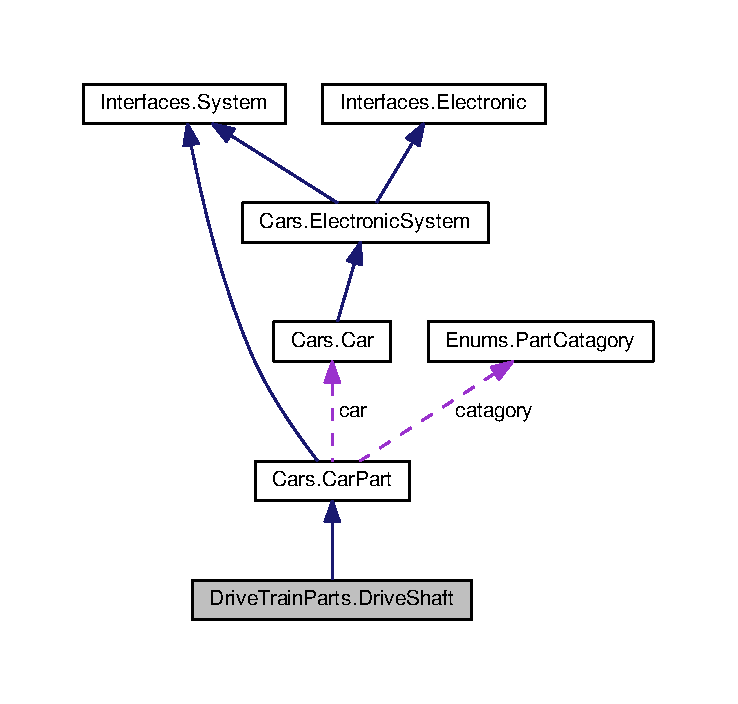
\includegraphics[width=350pt]{classDriveTrainParts_1_1DriveShaft__coll__graph}
\end{center}
\end{figure}
\subsection*{Public Member Functions}
\begin{DoxyCompactItemize}
\item 
\hypertarget{classDriveTrainParts_1_1DriveShaft_ae3ec3833a77c41c630b3f178bea50879}{}{\bfseries Drive\+Shaft} (\hyperlink{classCars_1_1Car}{Car} c, \hyperlink{enumEnums_1_1Location}{Location} loc)\label{classDriveTrainParts_1_1DriveShaft_ae3ec3833a77c41c630b3f178bea50879}

\end{DoxyCompactItemize}
\subsection*{Additional Inherited Members}


The documentation for this class was generated from the following file\+:\begin{DoxyCompactItemize}
\item 
src/\+Drive\+Train\+Parts/Drive\+Shaft.\+java\end{DoxyCompactItemize}

\hypertarget{classSystems_1_1DriveTrain}{}\section{Systems.\+Drive\+Train Class Reference}
\label{classSystems_1_1DriveTrain}\index{Systems.\+Drive\+Train@{Systems.\+Drive\+Train}}


Inheritance diagram for Systems.\+Drive\+Train\+:\nopagebreak
\begin{figure}[H]
\begin{center}
\leavevmode
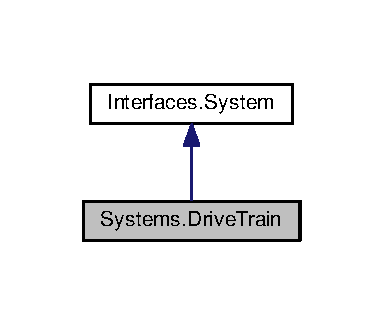
\includegraphics[width=184pt]{classSystems_1_1DriveTrain__inherit__graph}
\end{center}
\end{figure}


Collaboration diagram for Systems.\+Drive\+Train\+:
\nopagebreak
\begin{figure}[H]
\begin{center}
\leavevmode
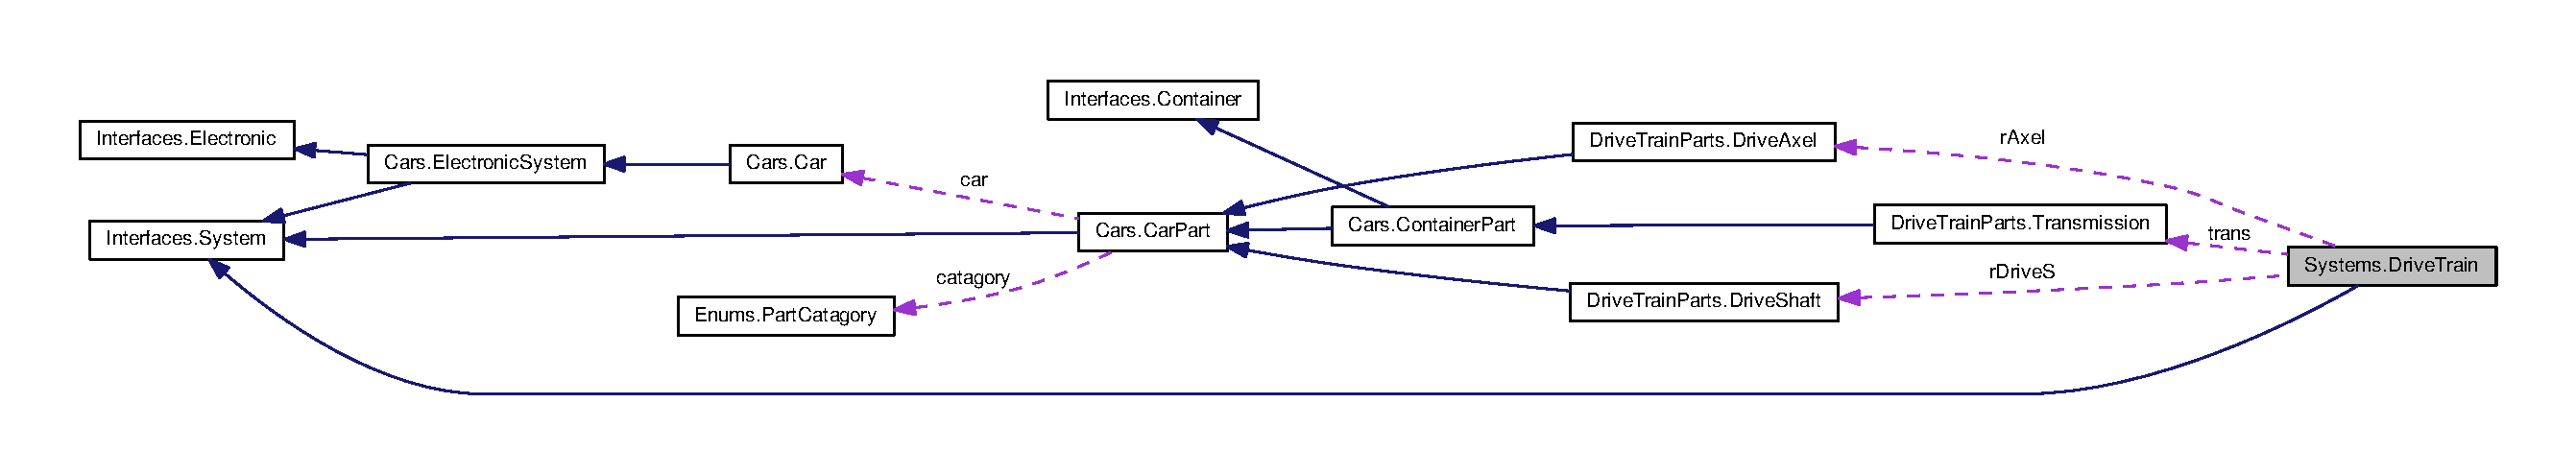
\includegraphics[width=350pt]{classSystems_1_1DriveTrain__coll__graph}
\end{center}
\end{figure}
\subsection*{Public Member Functions}
\begin{DoxyCompactItemize}
\item 
\hypertarget{classSystems_1_1DriveTrain_a527bae43081ca8617eaa5c29c7f14ab3}{}{\bfseries Drive\+Train} (\hyperlink{classCars_1_1Car}{Car} c, \hyperlink{enumEnums_1_1Location}{Location} loc)\label{classSystems_1_1DriveTrain_a527bae43081ca8617eaa5c29c7f14ab3}

\item 
\hypertarget{classSystems_1_1DriveTrain_a26af9fefa1f6076c5b762a919f3bc1f9}{}boolean {\bfseries operational} ()\label{classSystems_1_1DriveTrain_a26af9fefa1f6076c5b762a919f3bc1f9}

\item 
\hypertarget{classSystems_1_1DriveTrain_abc012f6fae9c4e930dfbe76b42c8c50e}{}boolean {\bfseries replace} (\hyperlink{classCars_1_1CarPart}{Car\+Part} old\+Part, \hyperlink{classCars_1_1CarPart}{Car\+Part} new\+Part)\label{classSystems_1_1DriveTrain_abc012f6fae9c4e930dfbe76b42c8c50e}

\item 
\hypertarget{classSystems_1_1DriveTrain_abb90a7b5c8b4267dd6eea45732fcc580}{}void {\bfseries diagnostic} ()\label{classSystems_1_1DriveTrain_abb90a7b5c8b4267dd6eea45732fcc580}

\item 
\hypertarget{classSystems_1_1DriveTrain_abc46e307afec231430038673ece547ef}{}void {\bfseries inspect} ()\label{classSystems_1_1DriveTrain_abc46e307afec231430038673ece547ef}

\end{DoxyCompactItemize}


The documentation for this class was generated from the following file\+:\begin{DoxyCompactItemize}
\item 
src/\+Systems/Drive\+Train.\+java\end{DoxyCompactItemize}

\hypertarget{classSystems_1_1Electrical}{}\section{Systems.\+Electrical Class Reference}
\label{classSystems_1_1Electrical}\index{Systems.\+Electrical@{Systems.\+Electrical}}


Inheritance diagram for Systems.\+Electrical\+:\nopagebreak
\begin{figure}[H]
\begin{center}
\leavevmode
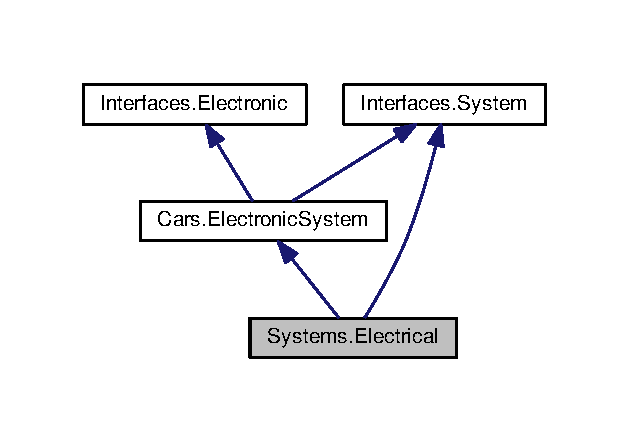
\includegraphics[width=302pt]{classSystems_1_1Electrical__inherit__graph}
\end{center}
\end{figure}


Collaboration diagram for Systems.\+Electrical\+:
\nopagebreak
\begin{figure}[H]
\begin{center}
\leavevmode
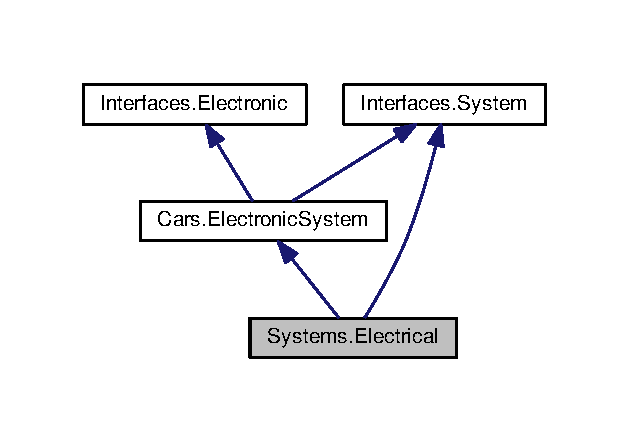
\includegraphics[width=302pt]{classSystems_1_1Electrical__coll__graph}
\end{center}
\end{figure}
\subsection*{Public Member Functions}
\begin{DoxyCompactItemize}
\item 
\hypertarget{classSystems_1_1Electrical_a8cf2687392c9cffc86c29ad9bdfe87a7}{}{\bfseries Electrical} (\hyperlink{classCars_1_1Car}{Car} car, \hyperlink{enumEnums_1_1Location}{Location} loc)\label{classSystems_1_1Electrical_a8cf2687392c9cffc86c29ad9bdfe87a7}

\item 
\hypertarget{classSystems_1_1Electrical_ab5662a428666e0a2516c5b6a790eea8f}{}boolean {\bfseries operation\+Loop} ()\label{classSystems_1_1Electrical_ab5662a428666e0a2516c5b6a790eea8f}

\item 
\hypertarget{classSystems_1_1Electrical_a5ac949e59eef886fecc63fdb0a07a765}{}boolean {\bfseries operational} ()\label{classSystems_1_1Electrical_a5ac949e59eef886fecc63fdb0a07a765}

\item 
\hypertarget{classSystems_1_1Electrical_ae50a9e1d9d3c147ffbd671ba5d392ad9}{}boolean {\bfseries replace} (\hyperlink{classCars_1_1CarPart}{Car\+Part} old\+Part, \hyperlink{classCars_1_1CarPart}{Car\+Part} new\+Part)\label{classSystems_1_1Electrical_ae50a9e1d9d3c147ffbd671ba5d392ad9}

\item 
\hypertarget{classSystems_1_1Electrical_a2e4138eb627e39556f04875eeafd93ae}{}void {\bfseries diagnostic} ()\label{classSystems_1_1Electrical_a2e4138eb627e39556f04875eeafd93ae}

\item 
\hypertarget{classSystems_1_1Electrical_a11ab42e38b1613d376b37d1976bd906f}{}void {\bfseries inspect} ()\label{classSystems_1_1Electrical_a11ab42e38b1613d376b37d1976bd906f}

\item 
\hypertarget{classSystems_1_1Electrical_a507954f14b94bfa1c3dd7df496cc4191}{}\hyperlink{classElectricalParts_1_1Battery}{Battery} {\bfseries get\+Battery} ()\label{classSystems_1_1Electrical_a507954f14b94bfa1c3dd7df496cc4191}

\item 
\hypertarget{classSystems_1_1Electrical_a1c6fa1a106c511db432925d9a9d5526a}{}\hyperlink{classConnectors_1_1Wire}{Wire} {\bfseries get\+Wire} ()\label{classSystems_1_1Electrical_a1c6fa1a106c511db432925d9a9d5526a}

\end{DoxyCompactItemize}
\subsection*{Additional Inherited Members}


The documentation for this class was generated from the following file\+:\begin{DoxyCompactItemize}
\item 
src/\+Systems/Electrical.\+java\end{DoxyCompactItemize}

\hypertarget{interfaceInterfaces_1_1Electronic}{}\section{Interfaces.\+Electronic Interface Reference}
\label{interfaceInterfaces_1_1Electronic}\index{Interfaces.\+Electronic@{Interfaces.\+Electronic}}


Inheritance diagram for Interfaces.\+Electronic\+:\nopagebreak
\begin{figure}[H]
\begin{center}
\leavevmode
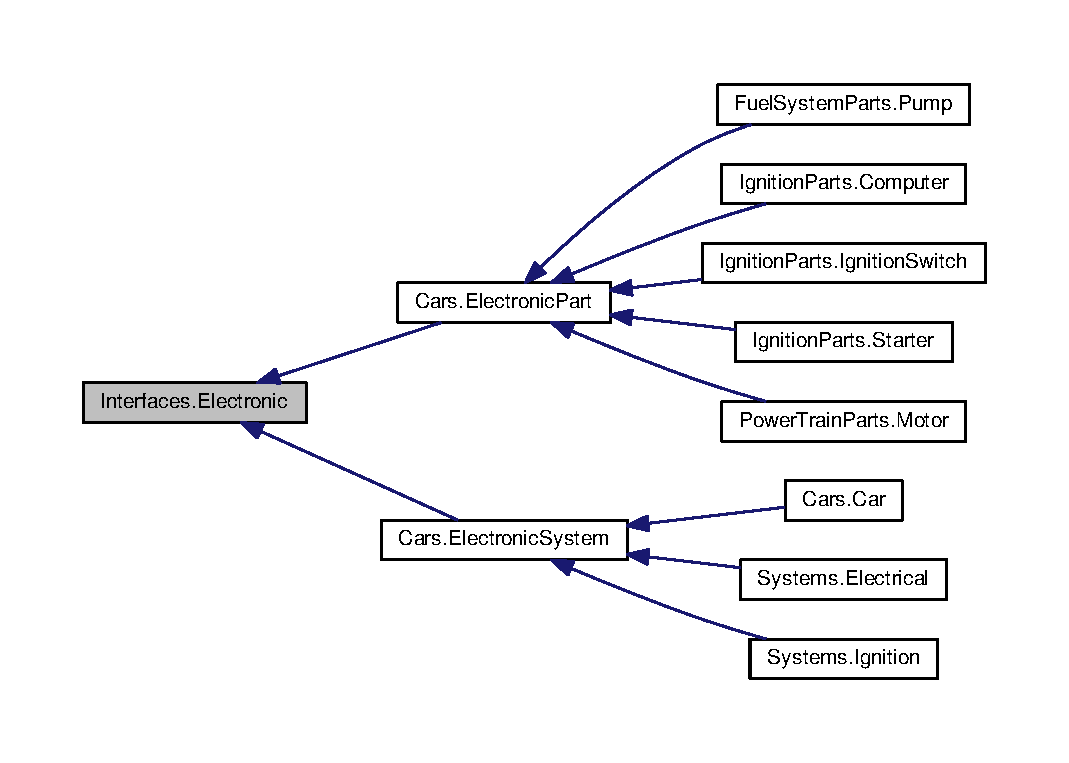
\includegraphics[width=350pt]{interfaceInterfaces_1_1Electronic__inherit__graph}
\end{center}
\end{figure}
\subsection*{Public Member Functions}
\begin{DoxyCompactItemize}
\item 
\hypertarget{interfaceInterfaces_1_1Electronic_ad3cbfe349692b0e1f546db7a1d3ecff2}{}boolean {\bfseries turn\+On} ()\label{interfaceInterfaces_1_1Electronic_ad3cbfe349692b0e1f546db7a1d3ecff2}

\item 
\hypertarget{interfaceInterfaces_1_1Electronic_a681234c8e833d9098bc947e033638aa8}{}boolean {\bfseries turn\+Off} ()\label{interfaceInterfaces_1_1Electronic_a681234c8e833d9098bc947e033638aa8}

\item 
\hypertarget{interfaceInterfaces_1_1Electronic_a7c76f201202f27a6ee9da422a294fadd}{}boolean {\bfseries run} ()\label{interfaceInterfaces_1_1Electronic_a7c76f201202f27a6ee9da422a294fadd}

\end{DoxyCompactItemize}


The documentation for this interface was generated from the following file\+:\begin{DoxyCompactItemize}
\item 
src/\+Interfaces/Electronic.\+java\end{DoxyCompactItemize}

\hypertarget{classCars_1_1ElectronicPart}{}\section{Cars.\+Electronic\+Part Class Reference}
\label{classCars_1_1ElectronicPart}\index{Cars.\+Electronic\+Part@{Cars.\+Electronic\+Part}}


Inheritance diagram for Cars.\+Electronic\+Part\+:\nopagebreak
\begin{figure}[H]
\begin{center}
\leavevmode
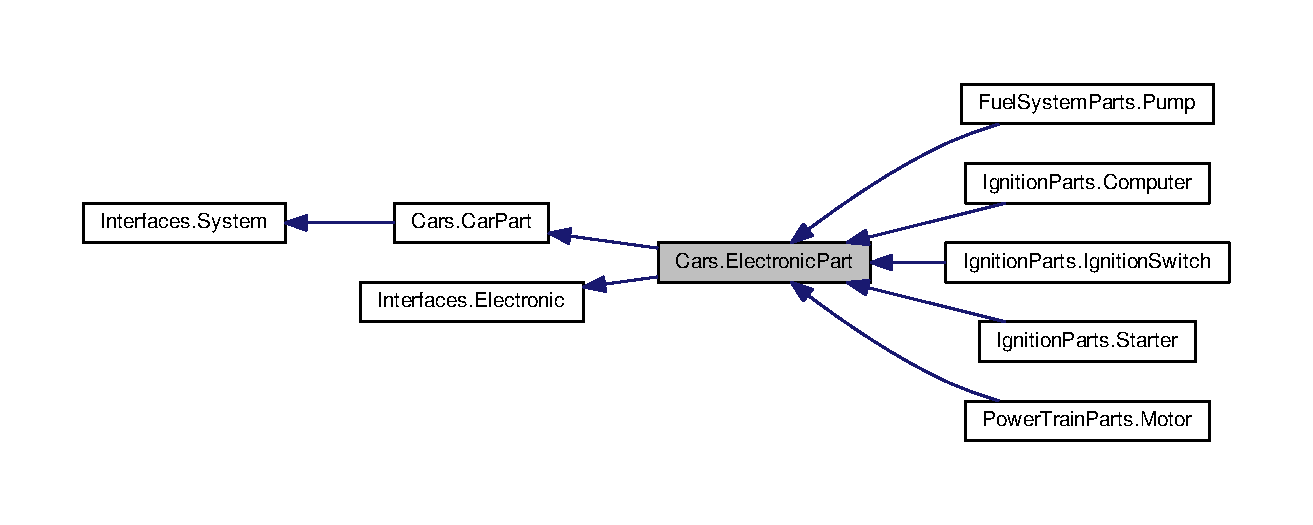
\includegraphics[width=350pt]{classCars_1_1ElectronicPart__inherit__graph}
\end{center}
\end{figure}


Collaboration diagram for Cars.\+Electronic\+Part\+:\nopagebreak
\begin{figure}[H]
\begin{center}
\leavevmode
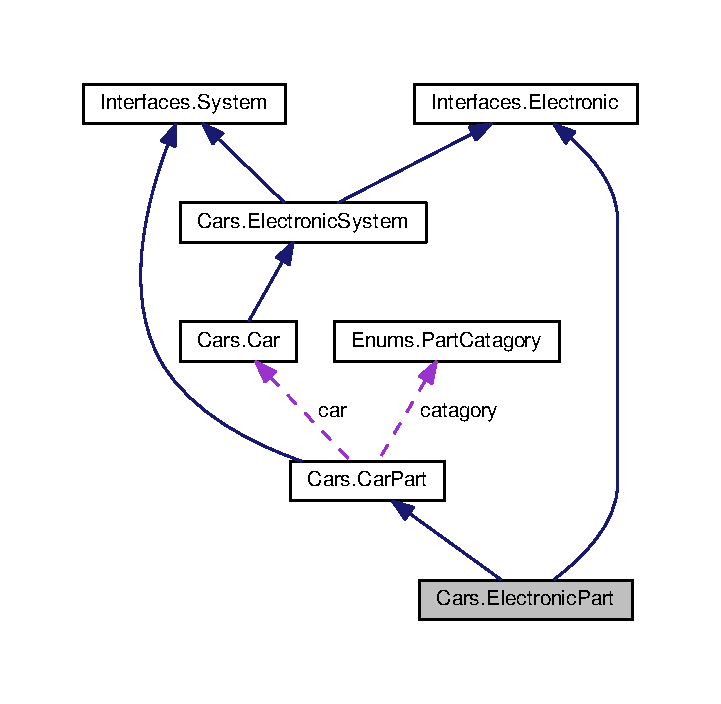
\includegraphics[width=346pt]{classCars_1_1ElectronicPart__coll__graph}
\end{center}
\end{figure}
\subsection*{Public Member Functions}
\begin{DoxyCompactItemize}
\item 
\hypertarget{classCars_1_1ElectronicPart_a476e83bd2cd79f0ebc7b3e9a73d53d39}{}{\bfseries Electronic\+Part} (\hyperlink{classCars_1_1Car}{Car} c, \hyperlink{enumEnums_1_1Location}{Location} loc)\label{classCars_1_1ElectronicPart_a476e83bd2cd79f0ebc7b3e9a73d53d39}

\item 
\hypertarget{classCars_1_1ElectronicPart_a1e10db7cf14215432b76ab9370c3a11f}{}boolean {\bfseries turn\+On} ()\label{classCars_1_1ElectronicPart_a1e10db7cf14215432b76ab9370c3a11f}

\item 
\hypertarget{classCars_1_1ElectronicPart_a244084d3e58c494fbbf3e466676b2450}{}boolean {\bfseries turn\+Off} ()\label{classCars_1_1ElectronicPart_a244084d3e58c494fbbf3e466676b2450}

\item 
\hypertarget{classCars_1_1ElectronicPart_a4dba4495835b001131f5c9fd668771eb}{}abstract boolean {\bfseries operation\+Loop} ()\label{classCars_1_1ElectronicPart_a4dba4495835b001131f5c9fd668771eb}

\item 
\hypertarget{classCars_1_1ElectronicPart_abc59a05d00c47fb2214e88b1491dae49}{}boolean {\bfseries run} ()\label{classCars_1_1ElectronicPart_abc59a05d00c47fb2214e88b1491dae49}

\item 
\hypertarget{classCars_1_1ElectronicPart_abb2d2e03e6c9d079df55ad1e044b76b6}{}boolean {\bfseries keep\+Going} ()\label{classCars_1_1ElectronicPart_abb2d2e03e6c9d079df55ad1e044b76b6}

\item 
\hypertarget{classCars_1_1ElectronicPart_acfb3683ac09bb6e7b75e2ad1bcdc3e97}{}boolean {\bfseries set\+Sleep\+Time} (double st)\label{classCars_1_1ElectronicPart_acfb3683ac09bb6e7b75e2ad1bcdc3e97}

\item 
\hypertarget{classCars_1_1ElectronicPart_aa4f963bfb8b24c1fe2caa9b80d21e459}{}\hyperlink{classElectricalParts_1_1Battery}{Battery} {\bfseries get\+Battery} ()\label{classCars_1_1ElectronicPart_aa4f963bfb8b24c1fe2caa9b80d21e459}

\item 
\hypertarget{classCars_1_1ElectronicPart_a0c0fc319a9e94daa997bcb0e4df401ee}{}boolean {\bfseries is\+Running} ()\label{classCars_1_1ElectronicPart_a0c0fc319a9e94daa997bcb0e4df401ee}

\end{DoxyCompactItemize}
\subsection*{Static Public Member Functions}
\begin{DoxyCompactItemize}
\item 
\hypertarget{classCars_1_1ElectronicPart_ae1aab39bc1dab4d86505c15f7930aa1b}{}static Boolean {\bfseries sleep} (double mil\+Sec)\label{classCars_1_1ElectronicPart_ae1aab39bc1dab4d86505c15f7930aa1b}

\end{DoxyCompactItemize}
\subsection*{Additional Inherited Members}


The documentation for this class was generated from the following file\+:\begin{DoxyCompactItemize}
\item 
src/\+Cars/Electronic\+Part.\+java\end{DoxyCompactItemize}

\hypertarget{classCars_1_1ElectronicSystem}{}\section{Cars.\+Electronic\+System Class Reference}
\label{classCars_1_1ElectronicSystem}\index{Cars.\+Electronic\+System@{Cars.\+Electronic\+System}}


Inheritance diagram for Cars.\+Electronic\+System\+:\nopagebreak
\begin{figure}[H]
\begin{center}
\leavevmode
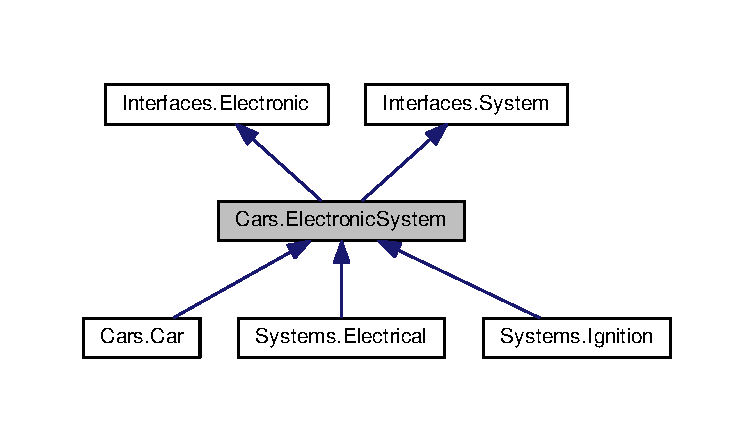
\includegraphics[width=350pt]{classCars_1_1ElectronicSystem__inherit__graph}
\end{center}
\end{figure}


Collaboration diagram for Cars.\+Electronic\+System\+:\nopagebreak
\begin{figure}[H]
\begin{center}
\leavevmode
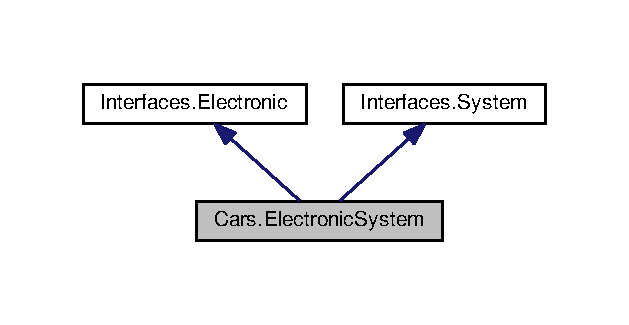
\includegraphics[width=302pt]{classCars_1_1ElectronicSystem__coll__graph}
\end{center}
\end{figure}
\subsection*{Public Member Functions}
\begin{DoxyCompactItemize}
\item 
\hypertarget{classCars_1_1ElectronicSystem_a80a3038f45fb00d70f53a9dc19b1e5b3}{}{\bfseries Electronic\+System} (\hyperlink{classCars_1_1Car}{Car} c, \hyperlink{enumEnums_1_1Location}{Location} loc)\label{classCars_1_1ElectronicSystem_a80a3038f45fb00d70f53a9dc19b1e5b3}

\item 
\hypertarget{classCars_1_1ElectronicSystem_a15f64be17364f391887970f2a87a1db9}{}boolean {\bfseries turn\+On} ()\label{classCars_1_1ElectronicSystem_a15f64be17364f391887970f2a87a1db9}

\item 
\hypertarget{classCars_1_1ElectronicSystem_a9974dafdd8c3d1f258bfa0f35a83abf8}{}boolean {\bfseries turn\+Off} ()\label{classCars_1_1ElectronicSystem_a9974dafdd8c3d1f258bfa0f35a83abf8}

\item 
\hypertarget{classCars_1_1ElectronicSystem_aade46607d4258acd492a6cca564bf670}{}abstract boolean {\bfseries operation\+Loop} ()\label{classCars_1_1ElectronicSystem_aade46607d4258acd492a6cca564bf670}

\item 
\hypertarget{classCars_1_1ElectronicSystem_a3b0b8750f418f490d0a4f01a4f0f2df4}{}boolean {\bfseries run} ()\label{classCars_1_1ElectronicSystem_a3b0b8750f418f490d0a4f01a4f0f2df4}

\item 
\hypertarget{classCars_1_1ElectronicSystem_aa01c93cb1ce7aa8a092dc9170f2eb275}{}boolean {\bfseries keep\+Going} ()\label{classCars_1_1ElectronicSystem_aa01c93cb1ce7aa8a092dc9170f2eb275}

\item 
\hypertarget{classCars_1_1ElectronicSystem_a107d134c7d4cb9a5dbaf90f3215b19f4}{}boolean {\bfseries set\+Sleep\+Time} (double st)\label{classCars_1_1ElectronicSystem_a107d134c7d4cb9a5dbaf90f3215b19f4}

\item 
\hypertarget{classCars_1_1ElectronicSystem_a72ab4114e0ffbcba610ade15aa451fc9}{}\hyperlink{classElectricalParts_1_1Battery}{Battery} {\bfseries get\+Battery} ()\label{classCars_1_1ElectronicSystem_a72ab4114e0ffbcba610ade15aa451fc9}

\item 
\hypertarget{classCars_1_1ElectronicSystem_adfa1b6d8c8590f23952bb252ec0f635c}{}boolean {\bfseries is\+Running} ()\label{classCars_1_1ElectronicSystem_adfa1b6d8c8590f23952bb252ec0f635c}

\item 
\hypertarget{classCars_1_1ElectronicSystem_ac320fbb5ee9da3e2ef62895c416af6ea}{}\hyperlink{classCars_1_1Car}{Car} {\bfseries get\+Car} ()\label{classCars_1_1ElectronicSystem_ac320fbb5ee9da3e2ef62895c416af6ea}

\end{DoxyCompactItemize}
\subsection*{Static Public Member Functions}
\begin{DoxyCompactItemize}
\item 
\hypertarget{classCars_1_1ElectronicSystem_a8ab7e7ed15db6c4bce5c5186a1fc3a93}{}static Boolean {\bfseries sleep} (double mil\+Sec)\label{classCars_1_1ElectronicSystem_a8ab7e7ed15db6c4bce5c5186a1fc3a93}

\end{DoxyCompactItemize}


The documentation for this class was generated from the following file\+:\begin{DoxyCompactItemize}
\item 
src/\+Cars/Electronic\+System.\+java\end{DoxyCompactItemize}

\hypertarget{classFuelSystemParts_1_1Filter}{}\section{Fuel\+System\+Parts.\+Filter Class Reference}
\label{classFuelSystemParts_1_1Filter}\index{Fuel\+System\+Parts.\+Filter@{Fuel\+System\+Parts.\+Filter}}


Inheritance diagram for Fuel\+System\+Parts.\+Filter\+:\nopagebreak
\begin{figure}[H]
\begin{center}
\leavevmode
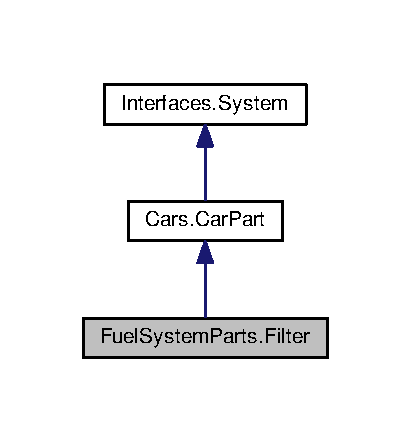
\includegraphics[width=197pt]{classFuelSystemParts_1_1Filter__inherit__graph}
\end{center}
\end{figure}


Collaboration diagram for Fuel\+System\+Parts.\+Filter\+:\nopagebreak
\begin{figure}[H]
\begin{center}
\leavevmode
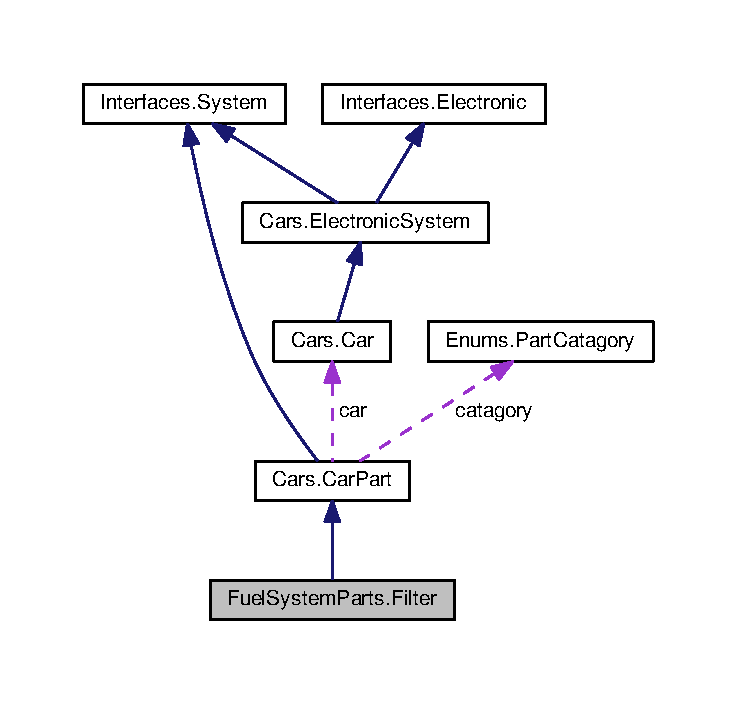
\includegraphics[width=350pt]{classFuelSystemParts_1_1Filter__coll__graph}
\end{center}
\end{figure}
\subsection*{Public Member Functions}
\begin{DoxyCompactItemize}
\item 
\hypertarget{classFuelSystemParts_1_1Filter_a6424e9860b6d9740c1fd6c12f0f9bf21}{}{\bfseries Filter} (\hyperlink{classCars_1_1Car}{Car} c, \hyperlink{enumEnums_1_1Location}{Location} loc)\label{classFuelSystemParts_1_1Filter_a6424e9860b6d9740c1fd6c12f0f9bf21}

\end{DoxyCompactItemize}
\subsection*{Additional Inherited Members}


The documentation for this class was generated from the following file\+:\begin{DoxyCompactItemize}
\item 
src/\+Fuel\+System\+Parts/Filter.\+java\end{DoxyCompactItemize}

\hypertarget{classSystems_1_1Fuel}{}\section{Systems.\+Fuel Class Reference}
\label{classSystems_1_1Fuel}\index{Systems.\+Fuel@{Systems.\+Fuel}}


Inheritance diagram for Systems.\+Fuel\+:\nopagebreak
\begin{figure}[H]
\begin{center}
\leavevmode
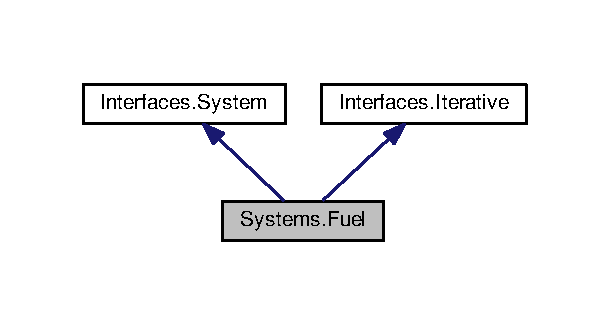
\includegraphics[width=293pt]{classSystems_1_1Fuel__inherit__graph}
\end{center}
\end{figure}


Collaboration diagram for Systems.\+Fuel\+:\nopagebreak
\begin{figure}[H]
\begin{center}
\leavevmode
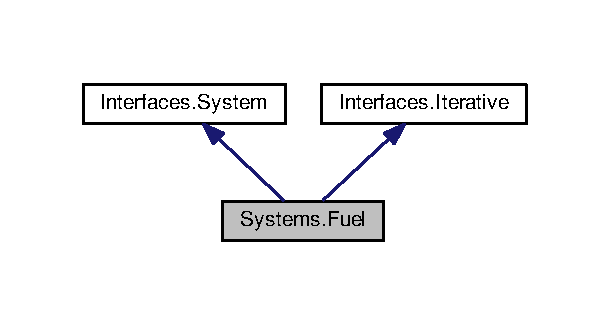
\includegraphics[width=293pt]{classSystems_1_1Fuel__coll__graph}
\end{center}
\end{figure}
\subsection*{Public Member Functions}
\begin{DoxyCompactItemize}
\item 
\hypertarget{classSystems_1_1Fuel_aec4d2cb06ca1feb0f5c7dc346f3d670a}{}{\bfseries Fuel} (\hyperlink{classCars_1_1Car}{Car} c, \hyperlink{enumEnums_1_1Location}{Location} loc)\label{classSystems_1_1Fuel_aec4d2cb06ca1feb0f5c7dc346f3d670a}

\item 
\hypertarget{classSystems_1_1Fuel_a5aae861a9a805c9d88ff0ac43484e7d2}{}boolean {\bfseries operational} ()\label{classSystems_1_1Fuel_a5aae861a9a805c9d88ff0ac43484e7d2}

\item 
\hypertarget{classSystems_1_1Fuel_a6eb19f16160cfd2d00ca17e4bd55d960}{}void {\bfseries diagnostic} ()\label{classSystems_1_1Fuel_a6eb19f16160cfd2d00ca17e4bd55d960}

\item 
\hypertarget{classSystems_1_1Fuel_ab993ea71389880a7ac6056bc2c3d27e1}{}void {\bfseries inspect} ()\label{classSystems_1_1Fuel_ab993ea71389880a7ac6056bc2c3d27e1}

\item 
\hypertarget{classSystems_1_1Fuel_ad3102e22490e5e86baaccfb4e98a428a}{}boolean {\bfseries replace} (\hyperlink{classCars_1_1CarPart}{Car\+Part} old\+Part, \hyperlink{classCars_1_1CarPart}{Car\+Part} new\+Part)\label{classSystems_1_1Fuel_ad3102e22490e5e86baaccfb4e98a428a}

\item 
\hypertarget{classSystems_1_1Fuel_a4f13df680679878b3b5ebee9f304bc73}{}void {\bfseries create} (String class\+Name, \hyperlink{enumEnums_1_1Location}{Location} locs)\label{classSystems_1_1Fuel_a4f13df680679878b3b5ebee9f304bc73}

\end{DoxyCompactItemize}


The documentation for this class was generated from the following file\+:\begin{DoxyCompactItemize}
\item 
src/\+Systems/Fuel.\+java\end{DoxyCompactItemize}

\hypertarget{classSystems_1_1Ignition}{}\section{Systems.\+Ignition Class Reference}
\label{classSystems_1_1Ignition}\index{Systems.\+Ignition@{Systems.\+Ignition}}


Inheritance diagram for Systems.\+Ignition\+:\nopagebreak
\begin{figure}[H]
\begin{center}
\leavevmode
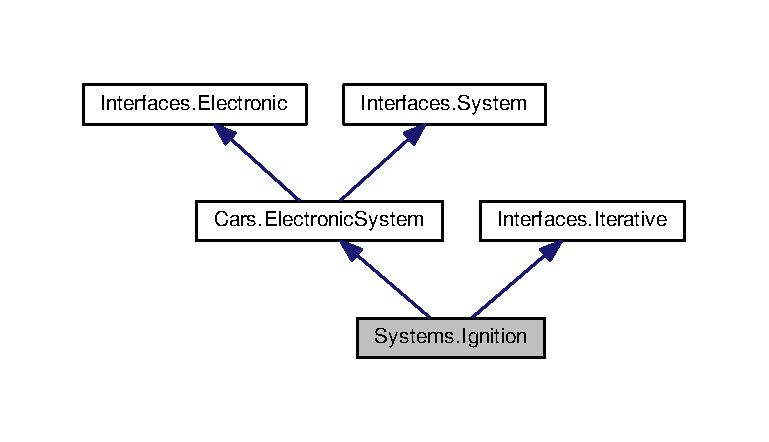
\includegraphics[width=350pt]{classSystems_1_1Ignition__inherit__graph}
\end{center}
\end{figure}


Collaboration diagram for Systems.\+Ignition\+:\nopagebreak
\begin{figure}[H]
\begin{center}
\leavevmode
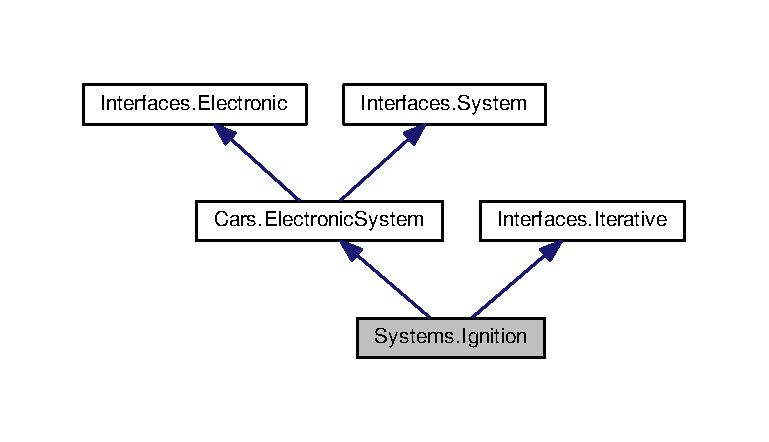
\includegraphics[width=350pt]{classSystems_1_1Ignition__coll__graph}
\end{center}
\end{figure}
\subsection*{Public Member Functions}
\begin{DoxyCompactItemize}
\item 
\hypertarget{classSystems_1_1Ignition_a708dc9c45f9c5f00c250281b94c1bfae}{}{\bfseries Ignition} (\hyperlink{classCars_1_1Car}{Car} car, \hyperlink{enumEnums_1_1Location}{Location} loc)\label{classSystems_1_1Ignition_a708dc9c45f9c5f00c250281b94c1bfae}

\item 
\hypertarget{classSystems_1_1Ignition_a88b183cbe5d44e0edb0fcdfc62f8f4ce}{}void {\bfseries create} (String class\+Name, \hyperlink{enumEnums_1_1Location}{Location} l)\label{classSystems_1_1Ignition_a88b183cbe5d44e0edb0fcdfc62f8f4ce}

\item 
\hypertarget{classSystems_1_1Ignition_a02bb30030dfc36e078911eac87f13e26}{}boolean {\bfseries operational} ()\label{classSystems_1_1Ignition_a02bb30030dfc36e078911eac87f13e26}

\item 
\hypertarget{classSystems_1_1Ignition_ac51b96fa23458e461fa8a97f0e8764cd}{}boolean {\bfseries replace} (\hyperlink{classCars_1_1CarPart}{Car\+Part} old\+Part, \hyperlink{classCars_1_1CarPart}{Car\+Part} new\+Part)\label{classSystems_1_1Ignition_ac51b96fa23458e461fa8a97f0e8764cd}

\item 
\hypertarget{classSystems_1_1Ignition_aa3b1a393839cbb267f20ceef4d1ebbdc}{}void {\bfseries diagnostic} ()\label{classSystems_1_1Ignition_aa3b1a393839cbb267f20ceef4d1ebbdc}

\item 
\hypertarget{classSystems_1_1Ignition_a41f2c709c74501bb2b5e17443633cea1}{}void {\bfseries inspect} ()\label{classSystems_1_1Ignition_a41f2c709c74501bb2b5e17443633cea1}

\item 
\hypertarget{classSystems_1_1Ignition_ab6ba7260e0b7481ce63808773438ba29}{}boolean {\bfseries operation\+Loop} ()\label{classSystems_1_1Ignition_ab6ba7260e0b7481ce63808773438ba29}

\item 
\hypertarget{classSystems_1_1Ignition_adc942df153ff686b31c00b37e3de4a13}{}void {\bfseries start} ()\label{classSystems_1_1Ignition_adc942df153ff686b31c00b37e3de4a13}

\item 
\hypertarget{classSystems_1_1Ignition_abcfa220a77b0b130bffbe94c2ac39fcd}{}\hyperlink{classElectricalParts_1_1Battery}{Battery} {\bfseries get\+Battery} ()\label{classSystems_1_1Ignition_abcfa220a77b0b130bffbe94c2ac39fcd}

\item 
\hypertarget{classSystems_1_1Ignition_ad1c383dc5f3eb96fc638c9edf586e529}{}boolean {\bfseries turn\+Off} ()\label{classSystems_1_1Ignition_ad1c383dc5f3eb96fc638c9edf586e529}

\end{DoxyCompactItemize}
\subsection*{Additional Inherited Members}


The documentation for this class was generated from the following file\+:\begin{DoxyCompactItemize}
\item 
src/\+Systems/Ignition.\+java\end{DoxyCompactItemize}

\hypertarget{classIgnitionParts_1_1IgnitionSwitch}{}\section{Ignition\+Parts.\+Ignition\+Switch Class Reference}
\label{classIgnitionParts_1_1IgnitionSwitch}\index{Ignition\+Parts.\+Ignition\+Switch@{Ignition\+Parts.\+Ignition\+Switch}}


Inheritance diagram for Ignition\+Parts.\+Ignition\+Switch\+:\nopagebreak
\begin{figure}[H]
\begin{center}
\leavevmode
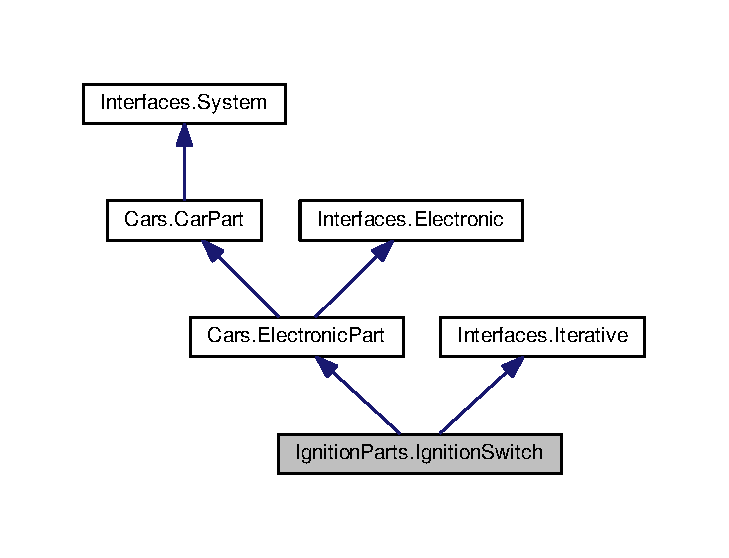
\includegraphics[width=350pt]{classIgnitionParts_1_1IgnitionSwitch__inherit__graph}
\end{center}
\end{figure}


Collaboration diagram for Ignition\+Parts.\+Ignition\+Switch\+:\nopagebreak
\begin{figure}[H]
\begin{center}
\leavevmode
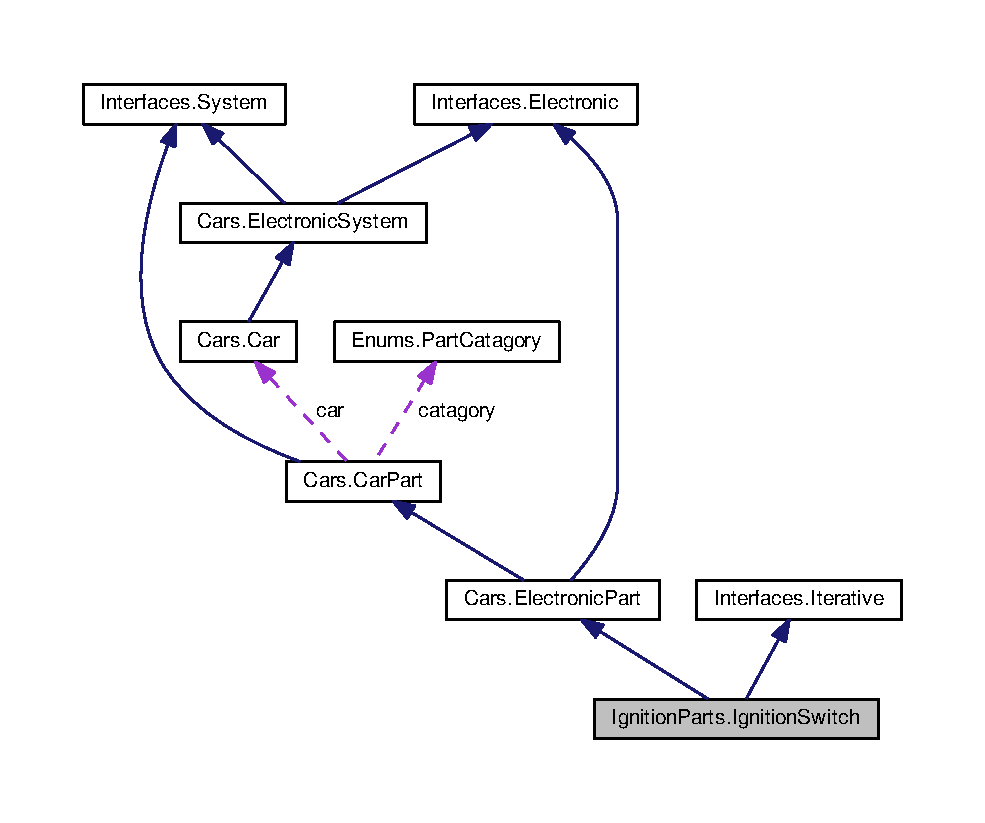
\includegraphics[width=350pt]{classIgnitionParts_1_1IgnitionSwitch__coll__graph}
\end{center}
\end{figure}
\subsection*{Public Member Functions}
\begin{DoxyCompactItemize}
\item 
\hypertarget{classIgnitionParts_1_1IgnitionSwitch_a4bc60395249312bdf34e31f026edf9fb}{}{\bfseries Ignition\+Switch} (\hyperlink{classCars_1_1Car}{Car} c, \hyperlink{enumEnums_1_1Location}{Location} loc)\label{classIgnitionParts_1_1IgnitionSwitch_a4bc60395249312bdf34e31f026edf9fb}

\item 
\hypertarget{classIgnitionParts_1_1IgnitionSwitch_a16dbac46fd19f70b949905108ed1cbb3}{}void {\bfseries create} (String class\+Name, \hyperlink{enumEnums_1_1Location}{Location} l)\label{classIgnitionParts_1_1IgnitionSwitch_a16dbac46fd19f70b949905108ed1cbb3}

\item 
\hypertarget{classIgnitionParts_1_1IgnitionSwitch_ab35e1290ccba8ff40eef971c56bc96c7}{}boolean {\bfseries operational} ()\label{classIgnitionParts_1_1IgnitionSwitch_ab35e1290ccba8ff40eef971c56bc96c7}

\item 
\hypertarget{classIgnitionParts_1_1IgnitionSwitch_ad9cc1014a08c9f12411e1fe5c064a4ff}{}boolean {\bfseries operation\+Loop} ()\label{classIgnitionParts_1_1IgnitionSwitch_ad9cc1014a08c9f12411e1fe5c064a4ff}

\item 
\hypertarget{classIgnitionParts_1_1IgnitionSwitch_ad00f4d11cedbdf9a4ea576134cd39aa4}{}void {\bfseries start} ()\label{classIgnitionParts_1_1IgnitionSwitch_ad00f4d11cedbdf9a4ea576134cd39aa4}

\item 
\hypertarget{classIgnitionParts_1_1IgnitionSwitch_a7d2dfa5d1c7efc65538b60cac41bf5b1}{}boolean {\bfseries turn\+Off} ()\label{classIgnitionParts_1_1IgnitionSwitch_a7d2dfa5d1c7efc65538b60cac41bf5b1}

\end{DoxyCompactItemize}
\subsection*{Additional Inherited Members}


The documentation for this class was generated from the following file\+:\begin{DoxyCompactItemize}
\item 
src/\+Ignition\+Parts/Ignition\+Switch.\+java\end{DoxyCompactItemize}

\hypertarget{interfaceInterfaces_1_1Iterative}{}\section{Interfaces.\+Iterative Interface Reference}
\label{interfaceInterfaces_1_1Iterative}\index{Interfaces.\+Iterative@{Interfaces.\+Iterative}}


Inheritance diagram for Interfaces.\+Iterative\+:\nopagebreak
\begin{figure}[H]
\begin{center}
\leavevmode
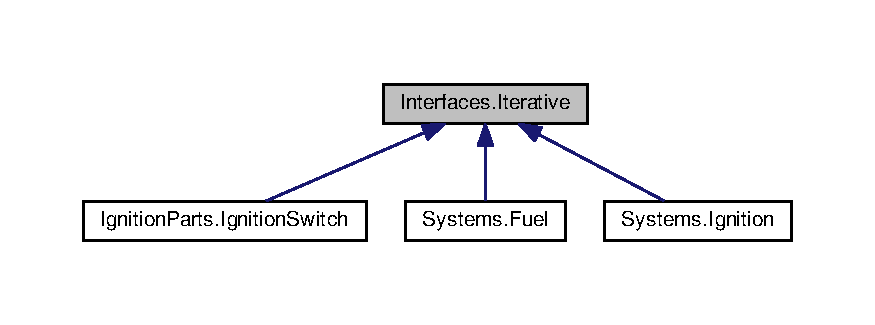
\includegraphics[width=350pt]{interfaceInterfaces_1_1Iterative__inherit__graph}
\end{center}
\end{figure}
\subsection*{Public Member Functions}
\begin{DoxyCompactItemize}
\item 
\hypertarget{interfaceInterfaces_1_1Iterative_a41e96d137f26a38b06cbbb79695bb96d}{}void {\bfseries create} (String class\+Name, \hyperlink{enumEnums_1_1Location}{Location} locs)\label{interfaceInterfaces_1_1Iterative_a41e96d137f26a38b06cbbb79695bb96d}

\end{DoxyCompactItemize}


The documentation for this interface was generated from the following file\+:\begin{DoxyCompactItemize}
\item 
src/\+Interfaces/Iterative.\+java\end{DoxyCompactItemize}

\hypertarget{classConnectors_1_1Line}{}\section{Connectors.\+Line Class Reference}
\label{classConnectors_1_1Line}\index{Connectors.\+Line@{Connectors.\+Line}}


Inheritance diagram for Connectors.\+Line\+:\nopagebreak
\begin{figure}[H]
\begin{center}
\leavevmode
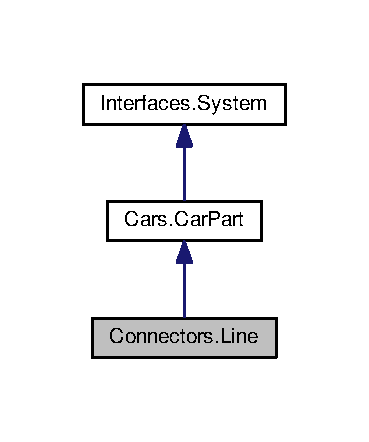
\includegraphics[width=177pt]{classConnectors_1_1Line__inherit__graph}
\end{center}
\end{figure}


Collaboration diagram for Connectors.\+Line\+:\nopagebreak
\begin{figure}[H]
\begin{center}
\leavevmode
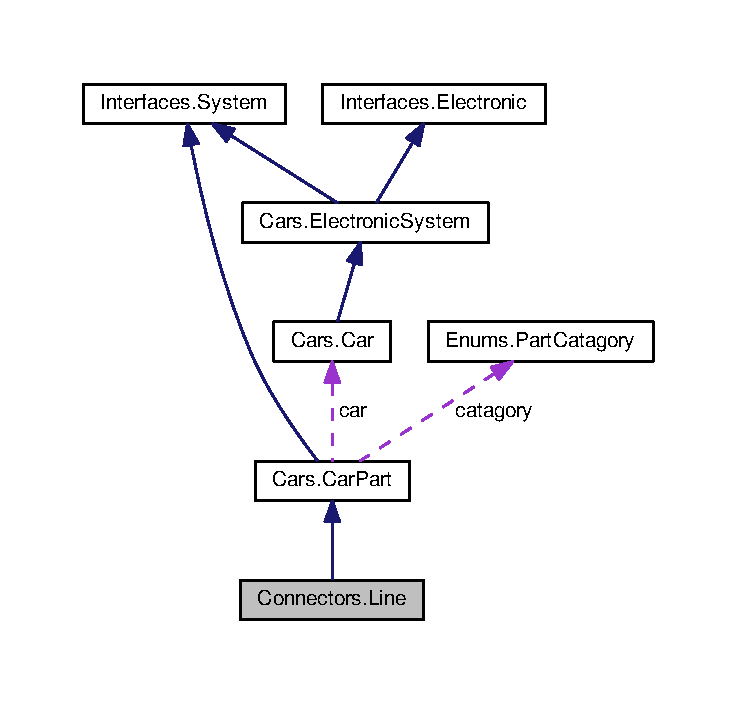
\includegraphics[width=350pt]{classConnectors_1_1Line__coll__graph}
\end{center}
\end{figure}
\subsection*{Public Member Functions}
\begin{DoxyCompactItemize}
\item 
\hypertarget{classConnectors_1_1Line_a400eaf106f8186364983486592e01707}{}{\bfseries Line} (\hyperlink{classCars_1_1Car}{Car} c, \hyperlink{enumEnums_1_1Location}{Location} loc)\label{classConnectors_1_1Line_a400eaf106f8186364983486592e01707}

\end{DoxyCompactItemize}
\subsection*{Additional Inherited Members}


The documentation for this class was generated from the following file\+:\begin{DoxyCompactItemize}
\item 
src/\+Connectors/Line.\+java\end{DoxyCompactItemize}

\hypertarget{enumEnums_1_1Location}{}\section{Enums.\+Location Enum Reference}
\label{enumEnums_1_1Location}\index{Enums.\+Location@{Enums.\+Location}}
\subsection*{Public Member Functions}
\begin{DoxyCompactItemize}
\item 
\hypertarget{enumEnums_1_1Location_afdfbde547421ed80e5c25973fbe0d141}{}\hyperlink{enumEnums_1_1Location}{Location} {\bfseries add\+Brake} (\hyperlink{enumEnums_1_1Location}{Location} other)\label{enumEnums_1_1Location_afdfbde547421ed80e5c25973fbe0d141}

\end{DoxyCompactItemize}
\subsection*{Public Attributes}
\begin{DoxyCompactItemize}
\item 
\hypertarget{enumEnums_1_1Location_a8c0405987010de1eb87632d90df32d2e}{}{\bfseries I\+N\+T\+E\+R\+I\+O\+R\+\_\+\+F\+R\+O\+N\+T}\label{enumEnums_1_1Location_a8c0405987010de1eb87632d90df32d2e}

\item 
\hypertarget{enumEnums_1_1Location_a536dc9f7f5cc25643ebc8816dd97590d}{}{\bfseries I\+N\+T\+E\+R\+I\+O\+R\+\_\+\+F\+R\+O\+N\+T\+\_\+\+D\+R\+I\+V\+E\+R\+S}\label{enumEnums_1_1Location_a536dc9f7f5cc25643ebc8816dd97590d}

\item 
\hypertarget{enumEnums_1_1Location_a82a18ad57ca1f0390a45032424a5a56b}{}{\bfseries I\+N\+T\+E\+R\+I\+O\+R\+\_\+\+F\+R\+O\+N\+T\+\_\+\+P\+A\+S\+S\+A\+N\+G\+E\+R\+S}\label{enumEnums_1_1Location_a82a18ad57ca1f0390a45032424a5a56b}

\item 
\hypertarget{enumEnums_1_1Location_acb0bf8d82387e65e3c19399b7f462354}{}{\bfseries I\+N\+T\+E\+R\+I\+O\+R\+\_\+\+R\+E\+A\+R}\label{enumEnums_1_1Location_acb0bf8d82387e65e3c19399b7f462354}

\item 
\hypertarget{enumEnums_1_1Location_a47b02b13137149d67e2bf56f172f496d}{}{\bfseries I\+N\+T\+E\+R\+I\+O\+R\+\_\+\+R\+E\+A\+R\+\_\+\+D\+R\+I\+V\+E\+R\+S}\label{enumEnums_1_1Location_a47b02b13137149d67e2bf56f172f496d}

\item 
\hypertarget{enumEnums_1_1Location_a872c13ad2d0fdaf334c5f8939aee75d7}{}{\bfseries I\+N\+T\+E\+R\+I\+O\+R\+\_\+\+R\+E\+A\+R\+\_\+\+P\+A\+S\+S\+A\+N\+G\+E\+R\+S}\label{enumEnums_1_1Location_a872c13ad2d0fdaf334c5f8939aee75d7}

\item 
\hypertarget{enumEnums_1_1Location_ae90f4f56d1b9ce59314c732366077e69}{}{\bfseries E\+X\+T\+E\+R\+I\+O\+R\+\_\+\+F\+R\+O\+N\+T}\label{enumEnums_1_1Location_ae90f4f56d1b9ce59314c732366077e69}

\item 
\hypertarget{enumEnums_1_1Location_a3abc1237150077cf4e979a69ad00b223}{}{\bfseries E\+X\+T\+E\+R\+I\+O\+R\+\_\+\+F\+R\+O\+N\+T\+\_\+\+D\+R\+I\+V\+E\+R\+S}\label{enumEnums_1_1Location_a3abc1237150077cf4e979a69ad00b223}

\item 
\hypertarget{enumEnums_1_1Location_a020dd9d9b0d4446778e482ba4ae3cdf5}{}{\bfseries E\+X\+T\+E\+R\+I\+O\+R\+\_\+\+F\+R\+O\+N\+T\+\_\+\+P\+A\+S\+S\+A\+N\+G\+E\+R\+S}\label{enumEnums_1_1Location_a020dd9d9b0d4446778e482ba4ae3cdf5}

\item 
\hypertarget{enumEnums_1_1Location_ade6f1d6a6a1b104ce44cb5c68cb0bc1e}{}{\bfseries E\+X\+T\+E\+R\+I\+O\+R\+\_\+\+R\+E\+A\+R}\label{enumEnums_1_1Location_ade6f1d6a6a1b104ce44cb5c68cb0bc1e}

\item 
\hypertarget{enumEnums_1_1Location_ae4cd8a3f2fb602455b938835a083515c}{}{\bfseries E\+X\+T\+E\+R\+I\+O\+R\+\_\+\+R\+E\+A\+R\+\_\+\+D\+R\+I\+V\+E\+R\+S}\label{enumEnums_1_1Location_ae4cd8a3f2fb602455b938835a083515c}

\item 
\hypertarget{enumEnums_1_1Location_ac01bf78e631edbd5e4ea3b158d2dcb4c}{}{\bfseries E\+X\+T\+E\+R\+I\+O\+R\+\_\+\+R\+E\+A\+R\+\_\+\+P\+A\+S\+S\+A\+N\+G\+E\+R\+S}\label{enumEnums_1_1Location_ac01bf78e631edbd5e4ea3b158d2dcb4c}

\item 
\hypertarget{enumEnums_1_1Location_ad3c641049489bcaea8b3d680d9575328}{}{\bfseries U\+N\+D\+E\+R\+C\+A\+R\+R\+I\+A\+G\+E\+\_\+\+C\+E\+N\+T\+E\+R}\label{enumEnums_1_1Location_ad3c641049489bcaea8b3d680d9575328}

\item 
\hypertarget{enumEnums_1_1Location_aabe6bf80be2ae7ac225179af8c15e26c}{}{\bfseries U\+N\+D\+E\+R\+C\+A\+R\+R\+I\+A\+G\+E\+\_\+\+F\+R\+O\+N\+T}\label{enumEnums_1_1Location_aabe6bf80be2ae7ac225179af8c15e26c}

\item 
\hypertarget{enumEnums_1_1Location_ae236d0d1a856f35711765306d502ee37}{}{\bfseries U\+N\+D\+E\+R\+C\+A\+R\+R\+I\+A\+G\+E\+\_\+\+F\+R\+O\+N\+T\+\_\+\+D\+R\+I\+V\+E\+R\+S}\label{enumEnums_1_1Location_ae236d0d1a856f35711765306d502ee37}

\item 
\hypertarget{enumEnums_1_1Location_a58e9ee84dacc5ca43e97824d067f0c16}{}{\bfseries U\+N\+D\+E\+R\+C\+A\+R\+R\+I\+A\+G\+E\+\_\+\+F\+R\+O\+N\+T\+\_\+\+P\+A\+S\+S\+A\+N\+G\+E\+R\+S}\label{enumEnums_1_1Location_a58e9ee84dacc5ca43e97824d067f0c16}

\item 
\hypertarget{enumEnums_1_1Location_af02c59baa614b42d5db0b4d70473aa3c}{}{\bfseries U\+N\+D\+E\+R\+C\+A\+R\+R\+I\+A\+G\+E\+\_\+\+R\+E\+A\+R}\label{enumEnums_1_1Location_af02c59baa614b42d5db0b4d70473aa3c}

\item 
\hypertarget{enumEnums_1_1Location_a5c4e347e7feddd1500209edf9c1a8694}{}{\bfseries U\+N\+D\+E\+R\+C\+A\+R\+R\+I\+A\+G\+E\+\_\+\+R\+E\+A\+R\+\_\+\+D\+R\+I\+V\+E\+R\+S}\label{enumEnums_1_1Location_a5c4e347e7feddd1500209edf9c1a8694}

\item 
\hypertarget{enumEnums_1_1Location_a9849f01a8704725eac4a6bbbc37b003a}{}{\bfseries U\+N\+D\+E\+R\+C\+A\+R\+R\+I\+A\+G\+E\+\_\+\+R\+E\+A\+R\+\_\+\+P\+A\+S\+S\+A\+N\+G\+E\+R\+S}\label{enumEnums_1_1Location_a9849f01a8704725eac4a6bbbc37b003a}

\item 
\hypertarget{enumEnums_1_1Location_a1e97ec32292cbcceb85c17c1b6c18fee}{}{\bfseries E\+N\+G\+I\+N\+E\+\_\+\+B\+A\+Y}\label{enumEnums_1_1Location_a1e97ec32292cbcceb85c17c1b6c18fee}

\item 
\hypertarget{enumEnums_1_1Location_adcdd255b1f47fca111a5360e7950e9e0}{}{\bfseries E\+N\+G\+I\+N\+E\+\_\+\+B\+A\+Y\+\_\+\+T\+O\+P}\label{enumEnums_1_1Location_adcdd255b1f47fca111a5360e7950e9e0}

\item 
\hypertarget{enumEnums_1_1Location_ad89fa12fc6603cb1b598491ccbbb5cd5}{}{\bfseries E\+N\+G\+I\+N\+E\+\_\+\+B\+A\+Y\+\_\+\+B\+O\+T\+T\+O\+M}\label{enumEnums_1_1Location_ad89fa12fc6603cb1b598491ccbbb5cd5}

\item 
\hypertarget{enumEnums_1_1Location_ab3b107a9ca613fef3f827e8bb5a63e54}{}{\bfseries S\+T\+O\+R\+A\+G\+E}\label{enumEnums_1_1Location_ab3b107a9ca613fef3f827e8bb5a63e54}

\item 
\hypertarget{enumEnums_1_1Location_a23a000d275a23614b8eee02e7de66fec}{}{\bfseries B\+F\+E}\label{enumEnums_1_1Location_a23a000d275a23614b8eee02e7de66fec}

\item 
\hypertarget{enumEnums_1_1Location_abad04f2de97dde1c3744fa784adc694a}{}{\bfseries T\+A\+N\+K\+\_\+\+T\+O\+\_\+\+F\+I\+L\+T\+E\+R}\label{enumEnums_1_1Location_abad04f2de97dde1c3744fa784adc694a}

\item 
\hypertarget{enumEnums_1_1Location_a8b897f5f024499b4e3ba1d75d47cb646}{}{\bfseries F\+I\+L\+T\+E\+R\+\_\+\+T\+O\+\_\+\+P\+U\+M\+P}\label{enumEnums_1_1Location_a8b897f5f024499b4e3ba1d75d47cb646}

\item 
\hypertarget{enumEnums_1_1Location_ac7d88ed4a90416a308f7b7882d3c5eb7}{}{\bfseries P\+U\+M\+P\+\_\+\+T\+O\+\_\+\+M\+O\+T\+O\+R}\label{enumEnums_1_1Location_ac7d88ed4a90416a308f7b7882d3c5eb7}

\item 
\hypertarget{enumEnums_1_1Location_a9a88ab4519717361f963945d93ff05c5}{}{\bfseries M\+A\+S\+T\+E\+R}\label{enumEnums_1_1Location_a9a88ab4519717361f963945d93ff05c5}

\item 
\hypertarget{enumEnums_1_1Location_ae4fe5b0026a9a83633786a2ba6c494f4}{}{\bfseries M\+A\+S\+T\+E\+R\+\_\+\+T\+O\+\_\+\+F\+R\+O\+N\+T\+\_\+\+D\+R\+I\+V\+E\+R\+S}\label{enumEnums_1_1Location_ae4fe5b0026a9a83633786a2ba6c494f4}

\item 
\hypertarget{enumEnums_1_1Location_a4a141b2d2026c572e32160a8d5cb8de1}{}{\bfseries M\+A\+S\+T\+E\+R\+\_\+\+T\+O\+\_\+\+F\+R\+O\+N\+T\+\_\+\+P\+A\+S\+S\+A\+N\+G\+E\+R\+S}\label{enumEnums_1_1Location_a4a141b2d2026c572e32160a8d5cb8de1}

\item 
\hypertarget{enumEnums_1_1Location_ad44211465d2a9e6e6f3bb0e0002c07af}{}{\bfseries M\+A\+S\+T\+E\+R\+\_\+\+T\+O\+\_\+\+R\+E\+A\+R\+\_\+\+D\+R\+I\+V\+E\+R\+S}\label{enumEnums_1_1Location_ad44211465d2a9e6e6f3bb0e0002c07af}

\item 
\hypertarget{enumEnums_1_1Location_ae99796ee117771f22ece92cafd94fae7}{}{\bfseries M\+A\+S\+T\+E\+R\+\_\+\+T\+O\+\_\+\+R\+E\+A\+R\+\_\+\+P\+A\+S\+S\+A\+N\+G\+E\+R\+S}\label{enumEnums_1_1Location_ae99796ee117771f22ece92cafd94fae7}

\item 
\hypertarget{enumEnums_1_1Location_a36aa7429cc3085cdc04e97c869cae49c}{}{\bfseries B\+A\+T\+T\+E\+R\+Y\+\_\+\+T\+O\+\_\+\+A\+L\+T\+E\+R\+N\+A\+T\+O\+R}\label{enumEnums_1_1Location_a36aa7429cc3085cdc04e97c869cae49c}

\item 
\hypertarget{enumEnums_1_1Location_aefee4b6d8ba82b4738e88a41169f19bc}{}{\bfseries B\+A\+T\+T\+E\+R\+Y\+\_\+\+T\+O\+\_\+\+C\+O\+M\+P\+U\+T\+E\+R}\label{enumEnums_1_1Location_aefee4b6d8ba82b4738e88a41169f19bc}

\item 
\hypertarget{enumEnums_1_1Location_a380d941442425f89134482e40aa04b1a}{}{\bfseries B\+A\+T\+T\+E\+R\+Y\+\_\+\+T\+O\+\_\+\+S\+T\+A\+R\+T\+E\+R}\label{enumEnums_1_1Location_a380d941442425f89134482e40aa04b1a}

\item 
\hypertarget{enumEnums_1_1Location_a42aa41714e73ef3367589e744767299a}{}{\bfseries B\+A\+T\+T\+E\+R\+Y\+\_\+\+T\+O\+\_\+\+F\+U\+E\+L\+\_\+\+P\+U\+M\+P}\label{enumEnums_1_1Location_a42aa41714e73ef3367589e744767299a}

\item 
\hypertarget{enumEnums_1_1Location_a6387bd1ff82f5182e80237b06aa1f62c}{}{\bfseries C\+O\+M\+P\+U\+T\+E\+R\+\_\+\+T\+O\+\_\+\+S\+T\+A\+R\+T\+E\+R}\label{enumEnums_1_1Location_a6387bd1ff82f5182e80237b06aa1f62c}

\item 
\hypertarget{enumEnums_1_1Location_a002bde27aed95c7ca43d9c2a649ab9e0}{}{\bfseries C\+O\+M\+P\+U\+T\+E\+R\+\_\+\+T\+O\+\_\+\+M\+O\+T\+O\+R}\label{enumEnums_1_1Location_a002bde27aed95c7ca43d9c2a649ab9e0}

\item 
\hypertarget{enumEnums_1_1Location_a0fdaa31f230abe7d2246e9be47329f88}{}{\bfseries C\+O\+M\+P\+U\+T\+E\+R\+\_\+\+T\+O\+\_\+\+I\+G\+N\+I\+T\+I\+O\+N\+\_\+\+S\+W\+I\+T\+C\+H}\label{enumEnums_1_1Location_a0fdaa31f230abe7d2246e9be47329f88}

\item 
\hypertarget{enumEnums_1_1Location_a54f4c973eda7c23daa2d4798a2dd01c1}{}{\bfseries B\+A\+T\+T\+E\+R\+Y\+\_\+\+T\+O\+\_\+\+I\+G\+N\+I\+T\+I\+O\+N}\label{enumEnums_1_1Location_a54f4c973eda7c23daa2d4798a2dd01c1}

\item 
\hypertarget{enumEnums_1_1Location_a904b45f5356d2cad686a41584038e53e}{}{\bfseries I\+G\+N\+I\+T\+I\+O\+N\+\_\+\+T\+O\+\_\+\+C\+O\+M\+P\+U\+T\+E\+R}\label{enumEnums_1_1Location_a904b45f5356d2cad686a41584038e53e}

\item 
\hypertarget{enumEnums_1_1Location_a11bbd0d76e5b4e9e52de8772c5eb3e21}{}{\bfseries I\+G\+N\+I\+T\+I\+O\+N\+\_\+\+T\+O\+\_\+\+S\+T\+A\+R\+T\+E\+R}\label{enumEnums_1_1Location_a11bbd0d76e5b4e9e52de8772c5eb3e21}

\item 
\hypertarget{enumEnums_1_1Location_a800ee70c357ad67398cdbb147450c889}{}{\bfseries T\+A\+N\+K\+\_\+\+T\+O\+\_\+\+M\+O\+T\+O\+R}\label{enumEnums_1_1Location_a800ee70c357ad67398cdbb147450c889}

\item 
\hypertarget{enumEnums_1_1Location_a8fa1b5fa22e86d2bf5d77fa9c03b94c1}{}{\bfseries M\+O\+T\+O\+R}\label{enumEnums_1_1Location_a8fa1b5fa22e86d2bf5d77fa9c03b94c1}

\item 
\hypertarget{enumEnums_1_1Location_a96c1b03c53864a085b5df209df55c11c}{}{\bfseries C\+A\+R}\label{enumEnums_1_1Location_a96c1b03c53864a085b5df209df55c11c}

\end{DoxyCompactItemize}


The documentation for this enum was generated from the following file\+:\begin{DoxyCompactItemize}
\item 
src/\+Enums/Location.\+java\end{DoxyCompactItemize}

\hypertarget{classBrakeParts_1_1MasterCylinder}{}\section{Brake\+Parts.\+Master\+Cylinder Class Reference}
\label{classBrakeParts_1_1MasterCylinder}\index{Brake\+Parts.\+Master\+Cylinder@{Brake\+Parts.\+Master\+Cylinder}}


Inheritance diagram for Brake\+Parts.\+Master\+Cylinder\+:
\nopagebreak
\begin{figure}[H]
\begin{center}
\leavevmode
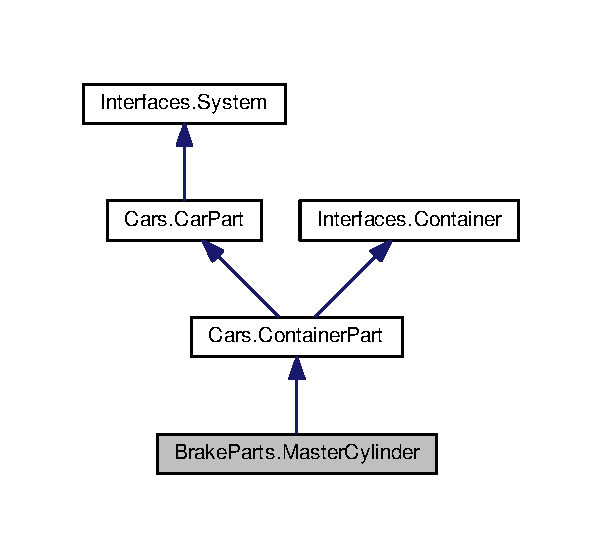
\includegraphics[width=289pt]{classBrakeParts_1_1MasterCylinder__inherit__graph}
\end{center}
\end{figure}


Collaboration diagram for Brake\+Parts.\+Master\+Cylinder\+:
\nopagebreak
\begin{figure}[H]
\begin{center}
\leavevmode
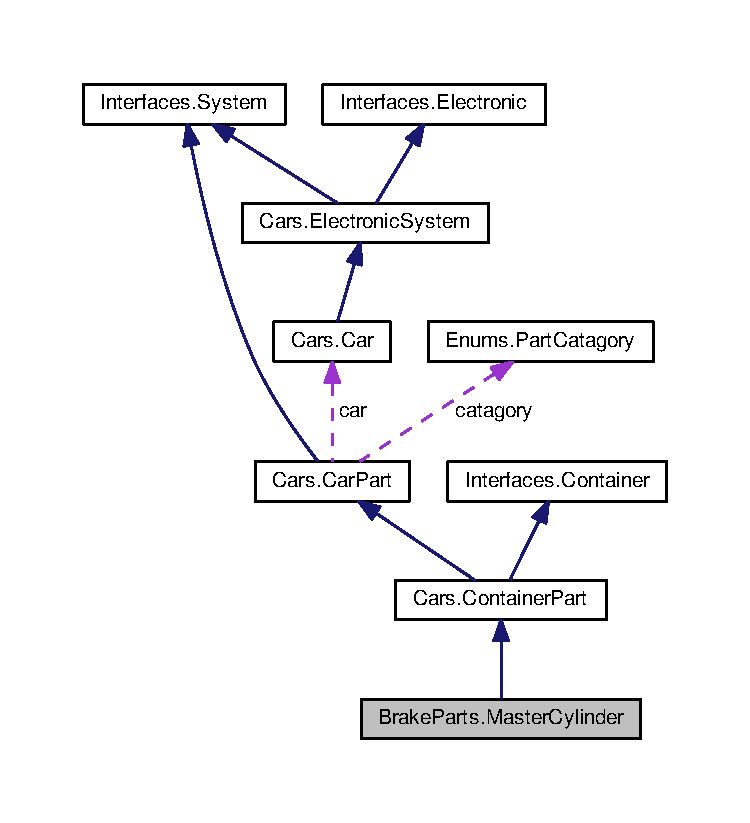
\includegraphics[width=350pt]{classBrakeParts_1_1MasterCylinder__coll__graph}
\end{center}
\end{figure}
\subsection*{Public Member Functions}
\begin{DoxyCompactItemize}
\item 
\hypertarget{classBrakeParts_1_1MasterCylinder_a7b0567a8c777405ac6a60e6d7ce19137}{}{\bfseries Master\+Cylinder} (\hyperlink{classCars_1_1Car}{Car} c, \hyperlink{enumEnums_1_1Location}{Location} loc)\label{classBrakeParts_1_1MasterCylinder_a7b0567a8c777405ac6a60e6d7ce19137}

\end{DoxyCompactItemize}
\subsection*{Additional Inherited Members}


The documentation for this class was generated from the following file\+:\begin{DoxyCompactItemize}
\item 
src/\+Brake\+Parts/Master\+Cylinder.\+java\end{DoxyCompactItemize}

\hypertarget{classPowerTrainParts_1_1Motor}{}\section{Power\+Train\+Parts.\+Motor Class Reference}
\label{classPowerTrainParts_1_1Motor}\index{Power\+Train\+Parts.\+Motor@{Power\+Train\+Parts.\+Motor}}


Inheritance diagram for Power\+Train\+Parts.\+Motor\+:\nopagebreak
\begin{figure}[H]
\begin{center}
\leavevmode
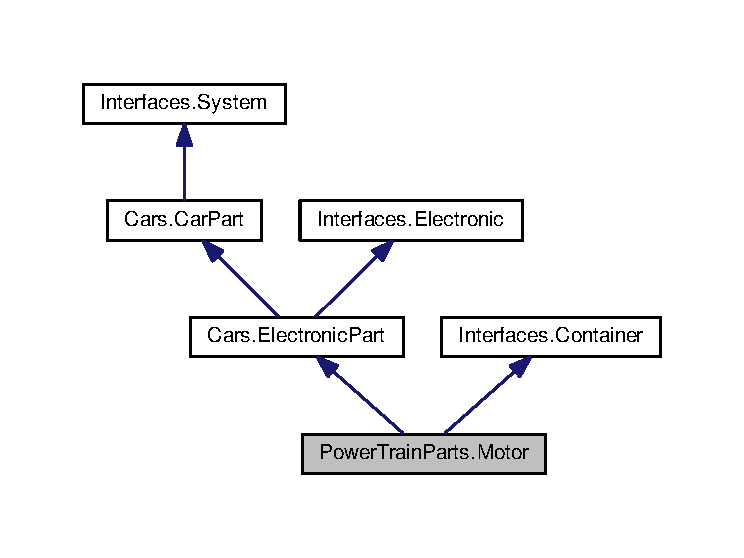
\includegraphics[width=350pt]{classPowerTrainParts_1_1Motor__inherit__graph}
\end{center}
\end{figure}


Collaboration diagram for Power\+Train\+Parts.\+Motor\+:\nopagebreak
\begin{figure}[H]
\begin{center}
\leavevmode
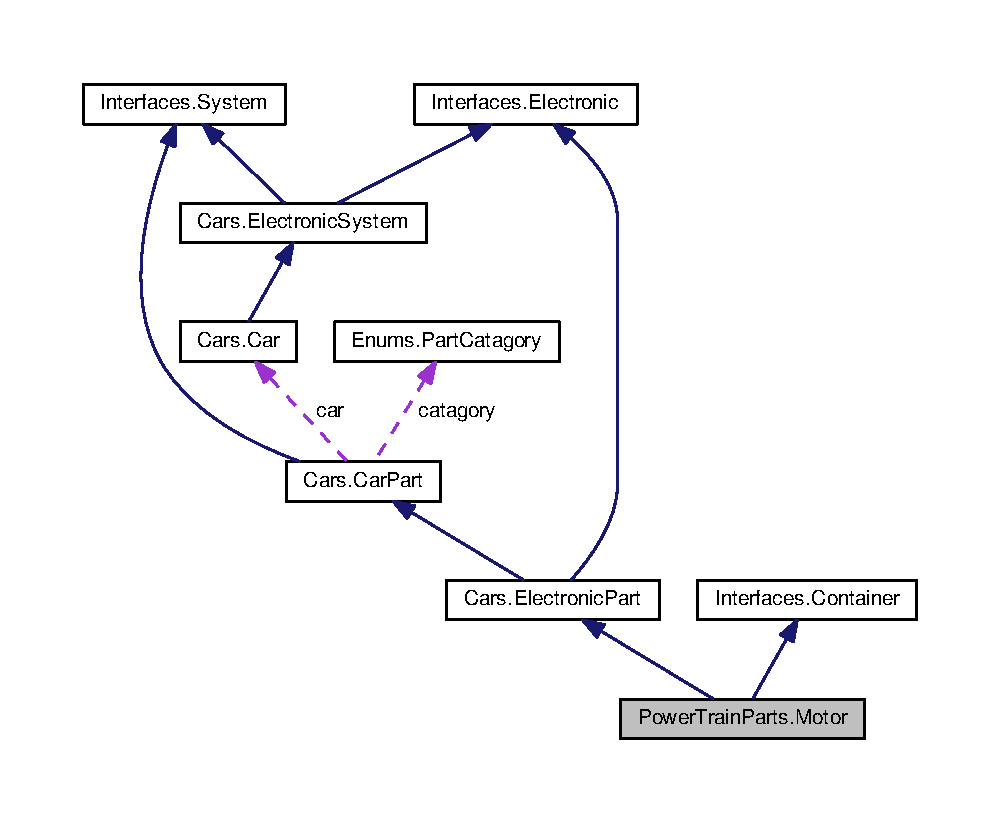
\includegraphics[width=350pt]{classPowerTrainParts_1_1Motor__coll__graph}
\end{center}
\end{figure}
\subsection*{Public Member Functions}
\begin{DoxyCompactItemize}
\item 
\hypertarget{classPowerTrainParts_1_1Motor_a5c320188ac1722fd18a4664566571a55}{}{\bfseries Motor} (\hyperlink{classCars_1_1Car}{Car} c, \hyperlink{enumEnums_1_1Location}{Location} loc)\label{classPowerTrainParts_1_1Motor_a5c320188ac1722fd18a4664566571a55}

\item 
\hypertarget{classPowerTrainParts_1_1Motor_a85639bd9914f0f8ab5c5ba65274afa03}{}boolean {\bfseries operational} ()\label{classPowerTrainParts_1_1Motor_a85639bd9914f0f8ab5c5ba65274afa03}

\item 
\hypertarget{classPowerTrainParts_1_1Motor_a76f3ccd355a02a56d24c8a8a2d2c1ae1}{}String {\bfseries check\+Level} ()\label{classPowerTrainParts_1_1Motor_a76f3ccd355a02a56d24c8a8a2d2c1ae1}

\item 
\hypertarget{classPowerTrainParts_1_1Motor_a805b4896f775c2cf38e16af9452aadba}{}double {\bfseries get\+Capacity} ()\label{classPowerTrainParts_1_1Motor_a805b4896f775c2cf38e16af9452aadba}

\item 
\hypertarget{classPowerTrainParts_1_1Motor_af917de0ecfc86bc75da51e8c0000ab02}{}void {\bfseries top\+Off} ()\label{classPowerTrainParts_1_1Motor_af917de0ecfc86bc75da51e8c0000ab02}

\item 
\hypertarget{classPowerTrainParts_1_1Motor_ae47c3c485c3e43235bbe395fa48f49b8}{}void {\bfseries replace\+Contents} ()\label{classPowerTrainParts_1_1Motor_ae47c3c485c3e43235bbe395fa48f49b8}

\item 
\hypertarget{classPowerTrainParts_1_1Motor_aed14d360795ca37c260d3665cbc60ae9}{}double {\bfseries get\+Last\+Flush} ()\label{classPowerTrainParts_1_1Motor_aed14d360795ca37c260d3665cbc60ae9}

\item 
\hypertarget{classPowerTrainParts_1_1Motor_a2fd035a5a6ac77fb80938db1d83f1bf7}{}boolean {\bfseries operation\+Loop} ()\label{classPowerTrainParts_1_1Motor_a2fd035a5a6ac77fb80938db1d83f1bf7}

\end{DoxyCompactItemize}
\subsection*{Protected Member Functions}
\begin{DoxyCompactItemize}
\item 
\hypertarget{classPowerTrainParts_1_1Motor_ac3d5a72f24cb136d954c5e887de689f9}{}void {\bfseries initialize} (double l, double c, double t, double fa)\label{classPowerTrainParts_1_1Motor_ac3d5a72f24cb136d954c5e887de689f9}

\end{DoxyCompactItemize}
\subsection*{Additional Inherited Members}


The documentation for this class was generated from the following file\+:\begin{DoxyCompactItemize}
\item 
src/\+Power\+Train\+Parts/Motor.\+java\end{DoxyCompactItemize}

\hypertarget{classPowerTrainParts_1_1OilFilter}{}\section{Power\+Train\+Parts.\+Oil\+Filter Class Reference}
\label{classPowerTrainParts_1_1OilFilter}\index{Power\+Train\+Parts.\+Oil\+Filter@{Power\+Train\+Parts.\+Oil\+Filter}}


Inheritance diagram for Power\+Train\+Parts.\+Oil\+Filter\+:\nopagebreak
\begin{figure}[H]
\begin{center}
\leavevmode
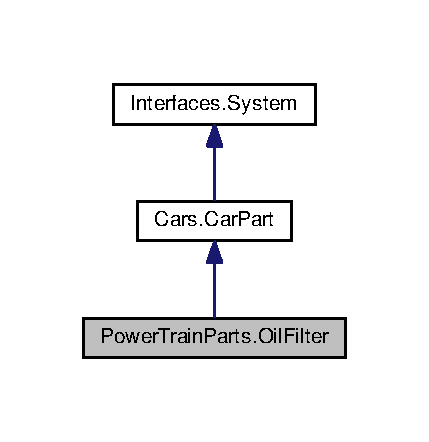
\includegraphics[width=206pt]{classPowerTrainParts_1_1OilFilter__inherit__graph}
\end{center}
\end{figure}


Collaboration diagram for Power\+Train\+Parts.\+Oil\+Filter\+:\nopagebreak
\begin{figure}[H]
\begin{center}
\leavevmode
\includegraphics[width=350pt]{classPowerTrainParts_1_1OilFilter__coll__graph}
\end{center}
\end{figure}
\subsection*{Public Member Functions}
\begin{DoxyCompactItemize}
\item 
\hypertarget{classPowerTrainParts_1_1OilFilter_a5ae9d4b867d983c9a4257c73800e66d6}{}{\bfseries Oil\+Filter} (\hyperlink{classCars_1_1Car}{Car} c, \hyperlink{enumEnums_1_1Location}{Location} loc)\label{classPowerTrainParts_1_1OilFilter_a5ae9d4b867d983c9a4257c73800e66d6}

\end{DoxyCompactItemize}
\subsection*{Additional Inherited Members}


The documentation for this class was generated from the following file\+:\begin{DoxyCompactItemize}
\item 
src/\+Power\+Train\+Parts/Oil\+Filter.\+java\end{DoxyCompactItemize}

\hypertarget{classBrakeParts_1_1Pads}{}\section{Brake\+Parts.\+Pads Class Reference}
\label{classBrakeParts_1_1Pads}\index{Brake\+Parts.\+Pads@{Brake\+Parts.\+Pads}}


Inheritance diagram for Brake\+Parts.\+Pads\+:\nopagebreak
\begin{figure}[H]
\begin{center}
\leavevmode
\includegraphics[width=177pt]{classBrakeParts_1_1Pads__inherit__graph}
\end{center}
\end{figure}


Collaboration diagram for Brake\+Parts.\+Pads\+:\nopagebreak
\begin{figure}[H]
\begin{center}
\leavevmode
\includegraphics[width=350pt]{classBrakeParts_1_1Pads__coll__graph}
\end{center}
\end{figure}
\subsection*{Public Member Functions}
\begin{DoxyCompactItemize}
\item 
\hypertarget{classBrakeParts_1_1Pads_a70cfbd2148157820ffd922dd21c6abf2}{}{\bfseries Pads} (\hyperlink{classCars_1_1Car}{Car} c, \hyperlink{enumEnums_1_1Location}{Location} loc)\label{classBrakeParts_1_1Pads_a70cfbd2148157820ffd922dd21c6abf2}

\item 
\hypertarget{classBrakeParts_1_1Pads_a1761c1fc50305faf97a1e6eb41810f85}{}void {\bfseries inspect} ()\label{classBrakeParts_1_1Pads_a1761c1fc50305faf97a1e6eb41810f85}

\item 
\hypertarget{classBrakeParts_1_1Pads_ab54aee108e7221108ca46b1311b6be6c}{}boolean {\bfseries operational} ()\label{classBrakeParts_1_1Pads_ab54aee108e7221108ca46b1311b6be6c}

\end{DoxyCompactItemize}
\subsection*{Additional Inherited Members}


The documentation for this class was generated from the following file\+:\begin{DoxyCompactItemize}
\item 
src/\+Brake\+Parts/Pads.\+java\end{DoxyCompactItemize}

\hypertarget{enumEnums_1_1PartCatagory}{}\section{Enums.\+Part\+Catagory Enum Reference}
\label{enumEnums_1_1PartCatagory}\index{Enums.\+Part\+Catagory@{Enums.\+Part\+Catagory}}
\subsection*{Public Attributes}
\begin{DoxyCompactItemize}
\item 
\hypertarget{enumEnums_1_1PartCatagory_a241234bd2366e76cb43fe3c153cfc72c}{}{\bfseries S\+U\+S\+P\+E\+N\+S\+I\+O\+N}\label{enumEnums_1_1PartCatagory_a241234bd2366e76cb43fe3c153cfc72c}

\item 
\hypertarget{enumEnums_1_1PartCatagory_a3b1e52804ab718efbb09a55fc276fa63}{}{\bfseries D\+R\+I\+V\+E\+\_\+\+T\+R\+A\+I\+N}\label{enumEnums_1_1PartCatagory_a3b1e52804ab718efbb09a55fc276fa63}

\item 
\hypertarget{enumEnums_1_1PartCatagory_a6a46aeb340cde3aadcabecbf393fde35}{}{\bfseries P\+O\+W\+E\+R\+\_\+\+T\+R\+A\+I\+N}\label{enumEnums_1_1PartCatagory_a6a46aeb340cde3aadcabecbf393fde35}

\item 
\hypertarget{enumEnums_1_1PartCatagory_ac8c73542d8fca2242ca571697b269119}{}{\bfseries B\+R\+A\+K\+E\+S}\label{enumEnums_1_1PartCatagory_ac8c73542d8fca2242ca571697b269119}

\item 
\hypertarget{enumEnums_1_1PartCatagory_ac51770d0c9849de28b5946b0f4c55a0e}{}{\bfseries F\+U\+E\+L}\label{enumEnums_1_1PartCatagory_ac51770d0c9849de28b5946b0f4c55a0e}

\item 
\hypertarget{enumEnums_1_1PartCatagory_a7ada07c6b7b5bf6a86771f63b1a68c7f}{}{\bfseries E\+L\+E\+C\+T\+R\+I\+C\+A\+L}\label{enumEnums_1_1PartCatagory_a7ada07c6b7b5bf6a86771f63b1a68c7f}

\item 
\hypertarget{enumEnums_1_1PartCatagory_ac7f34d5f50de583abe3b73beabfe7646}{}{\bfseries I\+G\+N\+I\+T\+I\+O\+N}\label{enumEnums_1_1PartCatagory_ac7f34d5f50de583abe3b73beabfe7646}

\item 
\hypertarget{enumEnums_1_1PartCatagory_a1b24e676fc4b6d4221763ca0949243be}{}{\bfseries S\+T\+O\+R\+A\+G\+E}\label{enumEnums_1_1PartCatagory_a1b24e676fc4b6d4221763ca0949243be}

\end{DoxyCompactItemize}


The documentation for this enum was generated from the following file\+:\begin{DoxyCompactItemize}
\item 
src/\+Enums/Part\+Catagory.\+java\end{DoxyCompactItemize}

\hypertarget{classSystems_1_1PowerTrain}{}\section{Systems.\+Power\+Train Class Reference}
\label{classSystems_1_1PowerTrain}\index{Systems.\+Power\+Train@{Systems.\+Power\+Train}}


Inheritance diagram for Systems.\+Power\+Train\+:\nopagebreak
\begin{figure}[H]
\begin{center}
\leavevmode
\includegraphics[width=188pt]{classSystems_1_1PowerTrain__inherit__graph}
\end{center}
\end{figure}


Collaboration diagram for Systems.\+Power\+Train\+:\nopagebreak
\begin{figure}[H]
\begin{center}
\leavevmode
\includegraphics[width=350pt]{classSystems_1_1PowerTrain__coll__graph}
\end{center}
\end{figure}
\subsection*{Public Member Functions}
\begin{DoxyCompactItemize}
\item 
\hypertarget{classSystems_1_1PowerTrain_a61bc328ef205d36c441342ff899de6d0}{}{\bfseries Power\+Train} (\hyperlink{classCars_1_1Car}{Car} c, \hyperlink{enumEnums_1_1Location}{Location} loc)\label{classSystems_1_1PowerTrain_a61bc328ef205d36c441342ff899de6d0}

\item 
\hypertarget{classSystems_1_1PowerTrain_abf8c02ac78cf1645001ff46505b43084}{}boolean {\bfseries operational} ()\label{classSystems_1_1PowerTrain_abf8c02ac78cf1645001ff46505b43084}

\item 
\hypertarget{classSystems_1_1PowerTrain_ac94f236f68a0cfe47e7d93bda0085171}{}void {\bfseries diagnostic} ()\label{classSystems_1_1PowerTrain_ac94f236f68a0cfe47e7d93bda0085171}

\item 
\hypertarget{classSystems_1_1PowerTrain_a59f989bb9c83a00a6debb9965b51daad}{}void {\bfseries inspect} ()\label{classSystems_1_1PowerTrain_a59f989bb9c83a00a6debb9965b51daad}

\item 
\hypertarget{classSystems_1_1PowerTrain_a4bb7f81e681e1243b8dd6978cd480eaa}{}boolean {\bfseries replace} (\hyperlink{classCars_1_1CarPart}{Car\+Part} old\+Part, \hyperlink{classCars_1_1CarPart}{Car\+Part} new\+Part)\label{classSystems_1_1PowerTrain_a4bb7f81e681e1243b8dd6978cd480eaa}

\end{DoxyCompactItemize}


The documentation for this class was generated from the following file\+:\begin{DoxyCompactItemize}
\item 
src/\+Systems/Power\+Train.\+java\end{DoxyCompactItemize}

\hypertarget{classFuelSystemParts_1_1Pump}{}\section{Fuel\+System\+Parts.\+Pump Class Reference}
\label{classFuelSystemParts_1_1Pump}\index{Fuel\+System\+Parts.\+Pump@{Fuel\+System\+Parts.\+Pump}}


Inheritance diagram for Fuel\+System\+Parts.\+Pump\+:\nopagebreak
\begin{figure}[H]
\begin{center}
\leavevmode
\includegraphics[width=291pt]{classFuelSystemParts_1_1Pump__inherit__graph}
\end{center}
\end{figure}


Collaboration diagram for Fuel\+System\+Parts.\+Pump\+:\nopagebreak
\begin{figure}[H]
\begin{center}
\leavevmode
\includegraphics[width=350pt]{classFuelSystemParts_1_1Pump__coll__graph}
\end{center}
\end{figure}
\subsection*{Public Member Functions}
\begin{DoxyCompactItemize}
\item 
\hypertarget{classFuelSystemParts_1_1Pump_af1319ff7e9f54845a6374dc4e20602b6}{}{\bfseries Pump} (\hyperlink{classCars_1_1Car}{Car} c, \hyperlink{enumEnums_1_1Location}{Location} loc)\label{classFuelSystemParts_1_1Pump_af1319ff7e9f54845a6374dc4e20602b6}

\item 
\hypertarget{classFuelSystemParts_1_1Pump_ab3f399f2a7862a88633002767d0976f1}{}boolean {\bfseries operational} ()\label{classFuelSystemParts_1_1Pump_ab3f399f2a7862a88633002767d0976f1}

\item 
\hypertarget{classFuelSystemParts_1_1Pump_a77442687a2297befe7badb11d09a7caf}{}boolean {\bfseries operation\+Loop} ()\label{classFuelSystemParts_1_1Pump_a77442687a2297befe7badb11d09a7caf}

\end{DoxyCompactItemize}
\subsection*{Additional Inherited Members}


The documentation for this class was generated from the following file\+:\begin{DoxyCompactItemize}
\item 
src/\+Fuel\+System\+Parts/Pump.\+java\end{DoxyCompactItemize}

\hypertarget{classSuspensionParts_1_1Rim}{}\section{Suspension\+Parts.\+Rim Class Reference}
\label{classSuspensionParts_1_1Rim}\index{Suspension\+Parts.\+Rim@{Suspension\+Parts.\+Rim}}


Inheritance diagram for Suspension\+Parts.\+Rim\+:\nopagebreak
\begin{figure}[H]
\begin{center}
\leavevmode
\includegraphics[width=192pt]{classSuspensionParts_1_1Rim__inherit__graph}
\end{center}
\end{figure}


Collaboration diagram for Suspension\+Parts.\+Rim\+:\nopagebreak
\begin{figure}[H]
\begin{center}
\leavevmode
\includegraphics[width=350pt]{classSuspensionParts_1_1Rim__coll__graph}
\end{center}
\end{figure}
\subsection*{Public Member Functions}
\begin{DoxyCompactItemize}
\item 
\hypertarget{classSuspensionParts_1_1Rim_a33de015026dde99b8082aa7a8387d60c}{}{\bfseries Rim} (\hyperlink{classCars_1_1Car}{Car} c, \hyperlink{enumEnums_1_1Location}{Location} loc)\label{classSuspensionParts_1_1Rim_a33de015026dde99b8082aa7a8387d60c}

\item 
\hypertarget{classSuspensionParts_1_1Rim_aac9a8947c36ab59e02633464cc059ab0}{}double {\bfseries get\+Diameter} ()\label{classSuspensionParts_1_1Rim_aac9a8947c36ab59e02633464cc059ab0}

\end{DoxyCompactItemize}
\subsection*{Additional Inherited Members}


The documentation for this class was generated from the following file\+:\begin{DoxyCompactItemize}
\item 
src/\+Suspension\+Parts/Rim.\+java\end{DoxyCompactItemize}

\hypertarget{classBrakeParts_1_1Rotor}{}\section{Brake\+Parts.\+Rotor Class Reference}
\label{classBrakeParts_1_1Rotor}\index{Brake\+Parts.\+Rotor@{Brake\+Parts.\+Rotor}}


Inheritance diagram for Brake\+Parts.\+Rotor\+:\nopagebreak
\begin{figure}[H]
\begin{center}
\leavevmode
\includegraphics[width=177pt]{classBrakeParts_1_1Rotor__inherit__graph}
\end{center}
\end{figure}


Collaboration diagram for Brake\+Parts.\+Rotor\+:\nopagebreak
\begin{figure}[H]
\begin{center}
\leavevmode
\includegraphics[width=350pt]{classBrakeParts_1_1Rotor__coll__graph}
\end{center}
\end{figure}
\subsection*{Public Member Functions}
\begin{DoxyCompactItemize}
\item 
\hypertarget{classBrakeParts_1_1Rotor_aa8072fe1733e9333d81109955b3bb25b}{}{\bfseries Rotor} (\hyperlink{classCars_1_1Car}{Car} c, \hyperlink{enumEnums_1_1Location}{Location} loc)\label{classBrakeParts_1_1Rotor_aa8072fe1733e9333d81109955b3bb25b}

\item 
\hypertarget{classBrakeParts_1_1Rotor_a449851eee6c2ead95bd0c2c846ce087a}{}void {\bfseries inspect} ()\label{classBrakeParts_1_1Rotor_a449851eee6c2ead95bd0c2c846ce087a}

\item 
\hypertarget{classBrakeParts_1_1Rotor_af41feb8b05d175429aa0af9bc4f737f2}{}boolean {\bfseries operational} ()\label{classBrakeParts_1_1Rotor_af41feb8b05d175429aa0af9bc4f737f2}

\end{DoxyCompactItemize}
\subsection*{Additional Inherited Members}


The documentation for this class was generated from the following file\+:\begin{DoxyCompactItemize}
\item 
src/\+Brake\+Parts/Rotor.\+java\end{DoxyCompactItemize}

\hypertarget{classSuspensionParts_1_1Shock}{}\section{Suspension\+Parts.\+Shock Class Reference}
\label{classSuspensionParts_1_1Shock}\index{Suspension\+Parts.\+Shock@{Suspension\+Parts.\+Shock}}


Inheritance diagram for Suspension\+Parts.\+Shock\+:\nopagebreak
\begin{figure}[H]
\begin{center}
\leavevmode
\includegraphics[width=202pt]{classSuspensionParts_1_1Shock__inherit__graph}
\end{center}
\end{figure}


Collaboration diagram for Suspension\+Parts.\+Shock\+:\nopagebreak
\begin{figure}[H]
\begin{center}
\leavevmode
\includegraphics[width=350pt]{classSuspensionParts_1_1Shock__coll__graph}
\end{center}
\end{figure}
\subsection*{Public Member Functions}
\begin{DoxyCompactItemize}
\item 
\hypertarget{classSuspensionParts_1_1Shock_a585cb108af7a7e48c825df94e0196b7d}{}{\bfseries Shock} (\hyperlink{classCars_1_1Car}{Car} c, \hyperlink{enumEnums_1_1Location}{Location} loc)\label{classSuspensionParts_1_1Shock_a585cb108af7a7e48c825df94e0196b7d}

\end{DoxyCompactItemize}
\subsection*{Additional Inherited Members}


The documentation for this class was generated from the following file\+:\begin{DoxyCompactItemize}
\item 
src/\+Suspension\+Parts/Shock.\+java\end{DoxyCompactItemize}

\hypertarget{classCars_1_1Simulator}{}\section{Cars.\+Simulator Class Reference}
\label{classCars_1_1Simulator}\index{Cars.\+Simulator@{Cars.\+Simulator}}
\subsection*{Static Public Member Functions}
\begin{DoxyCompactItemize}
\item 
\hypertarget{classCars_1_1Simulator_a6c6d389cb0280939fd53911c301188b6}{}static void {\bfseries main} (String\mbox{[}$\,$\mbox{]} args)\label{classCars_1_1Simulator_a6c6d389cb0280939fd53911c301188b6}

\item 
\hypertarget{classCars_1_1Simulator_a8fbd5040759a6fdb37d78c66a23855bd}{}static void {\bfseries alternator\+Test} ()\label{classCars_1_1Simulator_a8fbd5040759a6fdb37d78c66a23855bd}

\item 
\hypertarget{classCars_1_1Simulator_af250a3c4192de9390ff0c7ae39e99f6c}{}static void {\bfseries drain\+Battery\+With\+Starter} ()\label{classCars_1_1Simulator_af250a3c4192de9390ff0c7ae39e99f6c}

\end{DoxyCompactItemize}


The documentation for this class was generated from the following file\+:\begin{DoxyCompactItemize}
\item 
src/\+Cars/Simulator.\+java\end{DoxyCompactItemize}

\hypertarget{classIgnitionParts_1_1Starter}{}\section{Ignition\+Parts.\+Starter Class Reference}
\label{classIgnitionParts_1_1Starter}\index{Ignition\+Parts.\+Starter@{Ignition\+Parts.\+Starter}}


Inheritance diagram for Ignition\+Parts.\+Starter\+:\nopagebreak
\begin{figure}[H]
\begin{center}
\leavevmode
\includegraphics[width=291pt]{classIgnitionParts_1_1Starter__inherit__graph}
\end{center}
\end{figure}


Collaboration diagram for Ignition\+Parts.\+Starter\+:\nopagebreak
\begin{figure}[H]
\begin{center}
\leavevmode
\includegraphics[width=346pt]{classIgnitionParts_1_1Starter__coll__graph}
\end{center}
\end{figure}
\subsection*{Public Member Functions}
\begin{DoxyCompactItemize}
\item 
\hypertarget{classIgnitionParts_1_1Starter_a04c10a8d00bb49312bb2265ad5201c24}{}{\bfseries Starter} (\hyperlink{classCars_1_1Car}{Car} c, \hyperlink{enumEnums_1_1Location}{Location} loc)\label{classIgnitionParts_1_1Starter_a04c10a8d00bb49312bb2265ad5201c24}

\item 
\hypertarget{classIgnitionParts_1_1Starter_acb55c8090d71f159be7f4f9e49740906}{}boolean {\bfseries operational} ()\label{classIgnitionParts_1_1Starter_acb55c8090d71f159be7f4f9e49740906}

\item 
\hypertarget{classIgnitionParts_1_1Starter_ab281e11a365fa32cbee68e7c2832c8a0}{}boolean {\bfseries operation\+Loop} ()\label{classIgnitionParts_1_1Starter_ab281e11a365fa32cbee68e7c2832c8a0}

\end{DoxyCompactItemize}
\subsection*{Additional Inherited Members}


The documentation for this class was generated from the following file\+:\begin{DoxyCompactItemize}
\item 
src/\+Ignition\+Parts/Starter.\+java\end{DoxyCompactItemize}

\hypertarget{enumEnums_1_1Status}{}\section{Enums.\+Status Enum Reference}
\label{enumEnums_1_1Status}\index{Enums.\+Status@{Enums.\+Status}}
\subsection*{Public Member Functions}
\begin{DoxyCompactItemize}
\item 
\hypertarget{enumEnums_1_1Status_a81a39c332235bd2b8812e191ecabbbcf}{}String {\bfseries to\+String} ()\label{enumEnums_1_1Status_a81a39c332235bd2b8812e191ecabbbcf}

\end{DoxyCompactItemize}
\subsection*{Public Attributes}
\begin{DoxyCompactItemize}
\item 
\hypertarget{enumEnums_1_1Status_a5fa6a4e1ff5360295848cf0bc73e7f42}{}{\bfseries F\+U\+N\+C\+T\+I\+O\+N\+A\+L}\label{enumEnums_1_1Status_a5fa6a4e1ff5360295848cf0bc73e7f42}

\item 
\hypertarget{enumEnums_1_1Status_aecedef8c4559718a67d0c9c39cb7b968}{}{\bfseries K\+N\+O\+C\+K\+I\+N\+G\+\_\+\+S\+O\+U\+N\+D}\label{enumEnums_1_1Status_aecedef8c4559718a67d0c9c39cb7b968}

\item 
\hypertarget{enumEnums_1_1Status_ae07a3f58c3d32dfcb353ed32c8c91ef6}{}{\bfseries W\+H\+I\+N\+I\+N\+G\+\_\+\+S\+O\+U\+N\+D}\label{enumEnums_1_1Status_ae07a3f58c3d32dfcb353ed32c8c91ef6}

\item 
\hypertarget{enumEnums_1_1Status_aaeb89a837ae8eb34b8dbf6733668fda8}{}{\bfseries B\+R\+O\+K\+E\+N}\label{enumEnums_1_1Status_aaeb89a837ae8eb34b8dbf6733668fda8}

\item 
\hypertarget{enumEnums_1_1Status_a5ce7916da9e59cdc5392ad23bed2ff3d}{}{\bfseries C\+L\+O\+G\+G\+E\+D}\label{enumEnums_1_1Status_a5ce7916da9e59cdc5392ad23bed2ff3d}

\end{DoxyCompactItemize}


The documentation for this enum was generated from the following file\+:\begin{DoxyCompactItemize}
\item 
src/\+Enums/Status.\+java\end{DoxyCompactItemize}

\hypertarget{classSuspensionParts_1_1Strut}{}\section{Suspension\+Parts.\+Strut Class Reference}
\label{classSuspensionParts_1_1Strut}\index{Suspension\+Parts.\+Strut@{Suspension\+Parts.\+Strut}}


Inheritance diagram for Suspension\+Parts.\+Strut\+:\nopagebreak
\begin{figure}[H]
\begin{center}
\leavevmode
\includegraphics[width=195pt]{classSuspensionParts_1_1Strut__inherit__graph}
\end{center}
\end{figure}


Collaboration diagram for Suspension\+Parts.\+Strut\+:\nopagebreak
\begin{figure}[H]
\begin{center}
\leavevmode
\includegraphics[width=350pt]{classSuspensionParts_1_1Strut__coll__graph}
\end{center}
\end{figure}
\subsection*{Public Member Functions}
\begin{DoxyCompactItemize}
\item 
\hypertarget{classSuspensionParts_1_1Strut_a0166df0fda65136563b5c3c80b6cca11}{}{\bfseries Strut} (\hyperlink{classCars_1_1Car}{Car} c, \hyperlink{enumEnums_1_1Location}{Location} loc)\label{classSuspensionParts_1_1Strut_a0166df0fda65136563b5c3c80b6cca11}

\end{DoxyCompactItemize}
\subsection*{Additional Inherited Members}


The documentation for this class was generated from the following file\+:\begin{DoxyCompactItemize}
\item 
src/\+Suspension\+Parts/Strut.\+java\end{DoxyCompactItemize}

\hypertarget{classSystems_1_1Suspension}{}\section{Systems.\+Suspension Class Reference}
\label{classSystems_1_1Suspension}\index{Systems.\+Suspension@{Systems.\+Suspension}}


Inheritance diagram for Systems.\+Suspension\+:\nopagebreak
\begin{figure}[H]
\begin{center}
\leavevmode
\includegraphics[width=190pt]{classSystems_1_1Suspension__inherit__graph}
\end{center}
\end{figure}


Collaboration diagram for Systems.\+Suspension\+:
\nopagebreak
\begin{figure}[H]
\begin{center}
\leavevmode
\includegraphics[width=350pt]{classSystems_1_1Suspension__coll__graph}
\end{center}
\end{figure}
\subsection*{Public Member Functions}
\begin{DoxyCompactItemize}
\item 
\hypertarget{classSystems_1_1Suspension_a02c52ca922503e8767c440878c81d525}{}{\bfseries Suspension} (\hyperlink{classCars_1_1Car}{Car} car, \hyperlink{enumEnums_1_1Location}{Location} loc)\label{classSystems_1_1Suspension_a02c52ca922503e8767c440878c81d525}

\item 
\hypertarget{classSystems_1_1Suspension_acedd4b1e8d41edb2b50ac421d53a67e5}{}boolean {\bfseries operational} ()\label{classSystems_1_1Suspension_acedd4b1e8d41edb2b50ac421d53a67e5}

\item 
\hypertarget{classSystems_1_1Suspension_a8d5851986a37e773ed09d608db7faba2}{}boolean {\bfseries replace} (\hyperlink{classCars_1_1CarPart}{Car\+Part} old\+Part, \hyperlink{classCars_1_1CarPart}{Car\+Part} new\+Part)\label{classSystems_1_1Suspension_a8d5851986a37e773ed09d608db7faba2}

\item 
\hypertarget{classSystems_1_1Suspension_abed727bc0496355cf1c634482b8721ee}{}void {\bfseries diagnostic} ()\label{classSystems_1_1Suspension_abed727bc0496355cf1c634482b8721ee}

\item 
\hypertarget{classSystems_1_1Suspension_ac19fd8b57b8ed3d738b61f35e36d8ed5}{}void {\bfseries inspect} ()\label{classSystems_1_1Suspension_ac19fd8b57b8ed3d738b61f35e36d8ed5}

\end{DoxyCompactItemize}


The documentation for this class was generated from the following file\+:\begin{DoxyCompactItemize}
\item 
src/\+Systems/Suspension.\+java\end{DoxyCompactItemize}

\hypertarget{interfaceInterfaces_1_1System}{}\section{Interfaces.\+System Interface Reference}
\label{interfaceInterfaces_1_1System}\index{Interfaces.\+System@{Interfaces.\+System}}


Inheritance diagram for Interfaces.\+System\+:\nopagebreak
\begin{figure}[H]
\begin{center}
\leavevmode
\includegraphics[width=350pt]{interfaceInterfaces_1_1System__inherit__graph}
\end{center}
\end{figure}
\subsection*{Public Member Functions}
\begin{DoxyCompactItemize}
\item 
\hypertarget{interfaceInterfaces_1_1System_af4a4d024fc8d9ce772155f77b3362044}{}boolean {\bfseries operational} ()\label{interfaceInterfaces_1_1System_af4a4d024fc8d9ce772155f77b3362044}

\item 
\hypertarget{interfaceInterfaces_1_1System_abd08a456c6923198bcb3e735c7659060}{}boolean {\bfseries replace} (\hyperlink{classCars_1_1CarPart}{Car\+Part} old\+Part, \hyperlink{classCars_1_1CarPart}{Car\+Part} new\+Part)\label{interfaceInterfaces_1_1System_abd08a456c6923198bcb3e735c7659060}

\item 
\hypertarget{interfaceInterfaces_1_1System_a381d3a9ef08fdb1a448c70435ccca296}{}void {\bfseries diagnostic} ()\label{interfaceInterfaces_1_1System_a381d3a9ef08fdb1a448c70435ccca296}

\item 
\hypertarget{interfaceInterfaces_1_1System_a51756be35139aca6f384b4149f62f3f0}{}void {\bfseries inspect} ()\label{interfaceInterfaces_1_1System_a51756be35139aca6f384b4149f62f3f0}

\end{DoxyCompactItemize}


The documentation for this interface was generated from the following file\+:\begin{DoxyCompactItemize}
\item 
src/\+Interfaces/System.\+java\end{DoxyCompactItemize}

\hypertarget{classFuelSystemParts_1_1Tank}{}\section{Fuel\+System\+Parts.\+Tank Class Reference}
\label{classFuelSystemParts_1_1Tank}\index{Fuel\+System\+Parts.\+Tank@{Fuel\+System\+Parts.\+Tank}}


Inheritance diagram for Fuel\+System\+Parts.\+Tank\+:
\nopagebreak
\begin{figure}[H]
\begin{center}
\leavevmode
\includegraphics[width=325pt]{classFuelSystemParts_1_1Tank__inherit__graph}
\end{center}
\end{figure}


Collaboration diagram for Fuel\+System\+Parts.\+Tank\+:
\nopagebreak
\begin{figure}[H]
\begin{center}
\leavevmode
\includegraphics[width=350pt]{classFuelSystemParts_1_1Tank__coll__graph}
\end{center}
\end{figure}
\subsection*{Public Member Functions}
\begin{DoxyCompactItemize}
\item 
\hypertarget{classFuelSystemParts_1_1Tank_acfde50b0b363fd26bef4c1d7c9957be2}{}{\bfseries Tank} (\hyperlink{classCars_1_1Car}{Car} c, \hyperlink{enumEnums_1_1Location}{Location} loc)\label{classFuelSystemParts_1_1Tank_acfde50b0b363fd26bef4c1d7c9957be2}

\item 
\hypertarget{classFuelSystemParts_1_1Tank_a4004153aac241d2dcb6be3a6895913dd}{}void {\bfseries inspect} ()\label{classFuelSystemParts_1_1Tank_a4004153aac241d2dcb6be3a6895913dd}

\item 
\hypertarget{classFuelSystemParts_1_1Tank_aff282084e1b30f12ca10ca6c760a55c0}{}String {\bfseries check\+Level} ()\label{classFuelSystemParts_1_1Tank_aff282084e1b30f12ca10ca6c760a55c0}

\item 
\hypertarget{classFuelSystemParts_1_1Tank_a5bb105d8d2d4fe2784476cc938360edf}{}boolean {\bfseries operational} ()\label{classFuelSystemParts_1_1Tank_a5bb105d8d2d4fe2784476cc938360edf}

\end{DoxyCompactItemize}
\subsection*{Additional Inherited Members}


The documentation for this class was generated from the following file\+:\begin{DoxyCompactItemize}
\item 
src/\+Fuel\+System\+Parts/Tank.\+java\end{DoxyCompactItemize}

\hypertarget{classSuspensionParts_1_1Tire}{}\section{Suspension\+Parts.\+Tire Class Reference}
\label{classSuspensionParts_1_1Tire}\index{Suspension\+Parts.\+Tire@{Suspension\+Parts.\+Tire}}


Inheritance diagram for Suspension\+Parts.\+Tire\+:
\nopagebreak
\begin{figure}[H]
\begin{center}
\leavevmode
\includegraphics[width=289pt]{classSuspensionParts_1_1Tire__inherit__graph}
\end{center}
\end{figure}


Collaboration diagram for Suspension\+Parts.\+Tire\+:
\nopagebreak
\begin{figure}[H]
\begin{center}
\leavevmode
\includegraphics[width=350pt]{classSuspensionParts_1_1Tire__coll__graph}
\end{center}
\end{figure}
\subsection*{Public Member Functions}
\begin{DoxyCompactItemize}
\item 
\hypertarget{classSuspensionParts_1_1Tire_ab08ad9af8c909f4e4dad4c5e9e37bed9}{}{\bfseries Tire} (\hyperlink{classCars_1_1Car}{Car} c, \hyperlink{enumEnums_1_1Location}{Location} loc)\label{classSuspensionParts_1_1Tire_ab08ad9af8c909f4e4dad4c5e9e37bed9}

\item 
\hypertarget{classSuspensionParts_1_1Tire_a54efdf3388766984f75268c94d50767a}{}double {\bfseries get\+Diameter} ()\label{classSuspensionParts_1_1Tire_a54efdf3388766984f75268c94d50767a}

\end{DoxyCompactItemize}
\subsection*{Additional Inherited Members}


The documentation for this class was generated from the following file\+:\begin{DoxyCompactItemize}
\item 
src/\+Suspension\+Parts/Tire.\+java\end{DoxyCompactItemize}

\hypertarget{classDriveTrainParts_1_1Transmission}{}\section{Drive\+Train\+Parts.\+Transmission Class Reference}
\label{classDriveTrainParts_1_1Transmission}\index{Drive\+Train\+Parts.\+Transmission@{Drive\+Train\+Parts.\+Transmission}}


Inheritance diagram for Drive\+Train\+Parts.\+Transmission\+:
\nopagebreak
\begin{figure}[H]
\begin{center}
\leavevmode
\includegraphics[width=289pt]{classDriveTrainParts_1_1Transmission__inherit__graph}
\end{center}
\end{figure}


Collaboration diagram for Drive\+Train\+Parts.\+Transmission\+:
\nopagebreak
\begin{figure}[H]
\begin{center}
\leavevmode
\includegraphics[width=350pt]{classDriveTrainParts_1_1Transmission__coll__graph}
\end{center}
\end{figure}
\subsection*{Public Member Functions}
\begin{DoxyCompactItemize}
\item 
\hypertarget{classDriveTrainParts_1_1Transmission_a0a5ddee913d6a2f38e862fa7c6c6a2bd}{}{\bfseries Transmission} (\hyperlink{classCars_1_1Car}{Car} c, \hyperlink{enumEnums_1_1Location}{Location} loc)\label{classDriveTrainParts_1_1Transmission_a0a5ddee913d6a2f38e862fa7c6c6a2bd}

\end{DoxyCompactItemize}
\subsection*{Additional Inherited Members}


The documentation for this class was generated from the following file\+:\begin{DoxyCompactItemize}
\item 
src/\+Drive\+Train\+Parts/Transmission.\+java\end{DoxyCompactItemize}

\hypertarget{classConnectors_1_1Wire}{}\section{Connectors.\+Wire Class Reference}
\label{classConnectors_1_1Wire}\index{Connectors.\+Wire@{Connectors.\+Wire}}


Inheritance diagram for Connectors.\+Wire\+:\nopagebreak
\begin{figure}[H]
\begin{center}
\leavevmode
\includegraphics[width=177pt]{classConnectors_1_1Wire__inherit__graph}
\end{center}
\end{figure}


Collaboration diagram for Connectors.\+Wire\+:\nopagebreak
\begin{figure}[H]
\begin{center}
\leavevmode
\includegraphics[width=350pt]{classConnectors_1_1Wire__coll__graph}
\end{center}
\end{figure}
\subsection*{Public Member Functions}
\begin{DoxyCompactItemize}
\item 
\hypertarget{classConnectors_1_1Wire_aa76cc89eba376942be5f71fc3d068f09}{}{\bfseries Wire} (\hyperlink{classCars_1_1Car}{Car} c, \hyperlink{enumEnums_1_1Location}{Location} loc)\label{classConnectors_1_1Wire_aa76cc89eba376942be5f71fc3d068f09}

\end{DoxyCompactItemize}
\subsection*{Additional Inherited Members}


The documentation for this class was generated from the following file\+:\begin{DoxyCompactItemize}
\item 
src/\+Connectors/Wire.\+java\end{DoxyCompactItemize}

\hypertarget{classCars_1_1WorkerThread}{}\section{Cars.\+Worker\+Thread Class Reference}
\label{classCars_1_1WorkerThread}\index{Cars.\+Worker\+Thread@{Cars.\+Worker\+Thread}}


Inheritance diagram for Cars.\+Worker\+Thread\+:\nopagebreak
\begin{figure}[H]
\begin{center}
\leavevmode
\includegraphics[width=182pt]{classCars_1_1WorkerThread__inherit__graph}
\end{center}
\end{figure}


Collaboration diagram for Cars.\+Worker\+Thread\+:\nopagebreak
\begin{figure}[H]
\begin{center}
\leavevmode
\includegraphics[width=182pt]{classCars_1_1WorkerThread__coll__graph}
\end{center}
\end{figure}
\subsection*{Public Member Functions}
\begin{DoxyCompactItemize}
\item 
\hypertarget{classCars_1_1WorkerThread_a80938fed607c3ed72bc62aa3fea38668}{}{\bfseries Worker\+Thread} (\hyperlink{classCars_1_1ElectronicPart}{Electronic\+Part} ep)\label{classCars_1_1WorkerThread_a80938fed607c3ed72bc62aa3fea38668}

\item 
\hypertarget{classCars_1_1WorkerThread_ac1c921d1df056143278f80f61e61876f}{}{\bfseries Worker\+Thread} (\hyperlink{classCars_1_1ElectronicSystem}{Electronic\+System} s)\label{classCars_1_1WorkerThread_ac1c921d1df056143278f80f61e61876f}

\item 
\hypertarget{classCars_1_1WorkerThread_a0e258ed49726752d0ab24052e1c741cf}{}void {\bfseries run} ()\label{classCars_1_1WorkerThread_a0e258ed49726752d0ab24052e1c741cf}

\item 
\hypertarget{classCars_1_1WorkerThread_abe9783d3f3939e056e8af47ba8007c81}{}void {\bfseries set\+Thread} (Thread thr)\label{classCars_1_1WorkerThread_abe9783d3f3939e056e8af47ba8007c81}

\item 
\hypertarget{classCars_1_1WorkerThread_afebe58d37591400d2ed6b676cde24a73}{}Thread {\bfseries get\+Thread} ()\label{classCars_1_1WorkerThread_afebe58d37591400d2ed6b676cde24a73}

\end{DoxyCompactItemize}


The documentation for this class was generated from the following file\+:\begin{DoxyCompactItemize}
\item 
src/\+Cars/Worker\+Thread.\+java\end{DoxyCompactItemize}

%--- End generated contents ---

% Index
\backmatter
\newpage
\phantomsection
\clearemptydoublepage
\addcontentsline{toc}{chapter}{Index}
\printindex

\end{document}
